\section*{Organization of the appendix}
\label{sec:organ-suppl}

In this supplementary we first introduce notation in \Cref{sec:notation-1}.
We gather the proof of \Cref{thm:time_reversal_manifold} as well as additional derivations on score-based generative models and Riemannian manifolds.
In \cref{sec:prel-stoch-riem}, we recall basics on stochastic Riemannian geometry following \textcite{hsu2002stochastic}.
In \cref{sec:likel-comp}, we introduce an extension to the Riemannian setting of the likelihood computation techniques in diffusion models.
% Details about parametric vector fields are given in \Cref{sec:vector_field}.
% In \cref{sec:eigenf-eigenv-lapl}, we recall some basic facts about eigenvalues and eigenfunctions of the Laplace--Beltrami operator on the \(d\)-dimensional sphere and torus.
We present an extension of \Cref{alg:rsgm} using predictor-corrector schemes in \Cref{sec:predictor-corrector}.
In \cref{sec:time-reversal}, we prove the extension of the time-reversal formula to manifold in \Cref{thm:time_reversal_manifold}.
We prove the convergence of RSGM, i.e. \Cref{thm:weak_qualitative}, in \Cref{sec:convergence-rsgm}.
The proof of the manifold implicit score matching loaas, drawing links between the denoising score matching loss and the implicit score matching loss, is presented \cref{sec:manifold_ism_proof}.
% We provide a thorough comparison between our approach and the one of \textcite{rozen2021moser} in \Cref{sec:comp-with-moser}.
% We show how our method can be adapted to perform density estimation in \Cref{sec:dens-estim-with}.
% Extensions to conditional SGM and Schr\"odinger Bridges are discussed in \Cref{sec:extensions}.
% In \Cref{sec:non-compact}, we briefly discuss the non compact setting.
% Details on the stereographic SGM are given in \Cref{sec:stereo_exp}.
Experimental details are given in \cref{sec:exp_detail_rsgm}

\section{Notation}
\label{sec:notation-1}

We refer to \Cref{sec:prel-stoch-riem} for more details about the basic concepts of Riemannian geometry and stochastic processes.
In this section, we merely introduce the notation used in our work.
We postpone an introduction to stochastic processes on manifolds to \Cref{sec:stoch-diff-equat}.

In this work we always consider a smooth, connected and complete manifold \(\c{M}\).
We focus on the case of Riemannian manifolds, namely manifolds equipped with a metric \(g\).
Metrics \(g\) are smooth scalar product on the manifold allowing us to define the notion of \emph{distance} on a manifold.
We refer to \Cref{sec:prel-stoch-riem} for a precise definition and a discussion on metrics.
Given a smooth map \(f \in \mathrm{C}^\infty(\c{M}, \R)\), the gradient \(\nabla f\) is defined for any \(f:\c{M} \rightarrow \R\), \(x \in \c{M}, v \in \mathrm{T}_x\c{M}\), \(\langle \nabla f, v \rangle_g = \mathrm{d} f (v)\).
The distane \(d_\c{M}(x,y)\) is defined as the infimum of the length of all the curves on \(\c{M}\) joining \(x\) and \(y\).
Geodesics are path defined on \(\c{M}\) by a second order equation (and a starting point and speed).
This second order equation corresponds to the first order minimization of an \emph{energy} functional whose minimizers also minimize the length.
In \Cref{sec:prel-stoch-riem}, we introduce the notion of geodesics using parallel transport.
The exponential mapping \(\exp_x: \mathsf{U} \c{M} \to \c{M}\) with \(\mathsf{U} \subset \mathrm{T}_x \c{M}\) is such that \(\exp_x(v) = \gamma(1)\) with \(\gamma(1)\) the geodesics with initial condition \((x,v)\) at time \(t=1\).
Finally the volume form is a differentiable form of same degree as the dimension of \(\c{M}\).
Since \(\c{M}\) is an orientable Riemannian manifold there is a natural volume form defined using the metric \(g\), namely \(\omega(x) = \abs{g(x)}^{1/2} \mathrm{d} x_1 \wedge \dots \mathrm{d} x_d\).
In this paper, we abuse notation and denote by the volume form this natural volume form.

\section{Preliminaries on stochastic Riemannian geometry}
\label{sec:prel-stoch-riem}

In this section, we recall some basic facts on Riemannian geometry and stochastic Riemannian geometry.
We follow \textcite{hsu2002stochastic,lee2018introduction,lee2006riemannian} and refer to \textcite{lee2010introduction,lee2013smooth} for a general introduction to topological and smooth manifolds.
Throughout this section \(\c{M}\) is a \(d\)-dimensional smooth manifold, \(\TM\) its tangent bundle and \(\TM^*\) it cotangent bundle.
We denote \(\mathrm{C}^\infty(\c{M})\) the set of real-valued smooth functions on \(\c{M}\) and \(\c{X}(\c{M})\) the set of vector fields on \(\c{M}\).

\subsection{Tensor field, metric, connection and transport}
\label{sec:metr-conn-tens}

\paragraph{Tensor field and Riemannian metric}

For a vector space \(V\) let \(\mathrm{T}^{k, \ell}(V) = V^{\otimes k} \otimes (V^\star)^{\otimes \ell}\) with \(k, \ell \in \N\).
For any \(k, \ell \in \N\) we define the space of \((k,\ell)\)-tensors as \(\mathrm{T}^{k,\ell} \c{M} = \sqcup_{p \in \c{M}} \mathrm{T}^{k,\ell}(\mathrm{T}_p\c{M})\).
Note that \(\Gamma(\c{M}, \mathrm{T}^{0,0}\c{M}) = \mathrm{C}^\infty(\c{M})\), \(\c{X}(\c{M}) = \Gamma(\c{M}, \mathrm{T}^{1,0} \c{M})\) and that the space of \(1\)-form on \(\c{M}\) is given by \(\Gamma(\c{M}, \mathrm{T}^{0,1} \c{M})\), where \(\Gamma(\c{M}, V(\c{M}))\) is a section of a vector bundle \(V(\c{M})\) \parencite[see][Chapter 10]{lee2013smooth}.
For any \(k \in \N\), we denote \(\mathrm{T}^{\abs{k}} \c{M} = \sqcup_{j=0}^k \mathrm{T}^{j,k-j} \c{M}\).
\(\c{M}\) is said to be
a Riemannian manifold if there exists \(g \in \Gamma(\c{M}, \mathrm{T}^{0,2} \c{M})\) such that for
any \(x \in \c{M}\), \(g(x)\) is positive definite. \(g\) is called the Riemannian metric
of \(\c{M}\).
Every smooth manifold can be equipped with a Riemannian metric \cite[see][Proposition 2.4]{lee2018introduction}.
In local coordinates we define \(G = \{g_{i,j}\}_{1 \leq i,j \leq d} = \{g(X_i, X_j)\}_{1 \leq i,j \leq d}\), where \(\{X_i\}_{i=1}^d\) is a basis of the tangent space.
In what follows we consider that \(\c{M}\) is equipped with a metric \(g\) and for any \(X, Y \in \c{X}(\c{M})\) we denote \(\langle X,Y \rangle_{\c{M}} = g(X,Y)\).

\paragraph{Connection}
A connection \(\nabla\) is a mapping which allows one to differentiate vector fields with respect to other vector fields.
\(\nabla\) is a linear map
\(\nabla: \ \c{X}(\c{M}) \times \c{X}(\c{M}) \to \c{X}(\c{M})\).
In addition, we assume that \begin{enumerate*}[label=\roman*)] \item for any \(f \in \mathrm{C}^\infty(\c{M})\), \(X, Y \in \c{X}(\c{M})\), \(\nabla_{f X}(Y) = f \nabla_X Y\), \item for any \(f \in \mathrm{C}^\infty(\c{M})\), \(X, Y \in \c{X}(\c{M})\), \(\nabla_{X}(fY) = f \nabla_X Y + X(f) Y\).
\end{enumerate*}
Given a system of local coordinates, the Christoffel symbols \(\{\Gamma_{i,j}^k\}_{1 \leq i,j,k\leq d}\) are given for any \(i,j \in \{1, \dots, d\}\) by \(\nabla_{X_i}X_j = \sum_{k=1}^d \Gamma_{i,j}^k X_k\).
We also define the Levi--Civita connection \(\nabla\) by considering the additional two conditions: \begin{enumerate*}[label=\roman*)] \item \(\nabla\) is torsion-free, i.e. \ for any \(X, Y \in \c{X}(\c{M})\) we have \(\nabla_X Y - \nabla_Y X = [X,Y]\), where \([X,Y]\) is the Lie bracket between \(X\) and \(Y\), \item \(\nabla\) is compatible with the metric \(g\), i.e. \ for any \(X,Y,Z \in \c{X}(\c{M})\), \(X (\langle Y,Z \rangle_\c{M}) = \langle\nabla_X Y, Z\rangle_\c{M} + \langle Y, \nabla_X Z \rangle_\c{M}\).
\end{enumerate*}
We recall that the Levi--Civita connection is uniquely defined since for any \(X,Y,Z \in \c{X}(\c{M})\) we have \begin{align} 2 \innerprod{\nabla_X Y}{Z}_{\c{M}} & = X(\innerprod{Y}{Z}_{\c{M}}) + Y(\innerprod{Z}{X}_{\c{M}}) - Z(\innerprod{X}{Y}_{\c{M}}) \\ & \qquad \qquad + \innerprod{[X,Y]}{Z}_{\c{M}} - \innerprod{[Z,X]}{Y}_{\c{M}} - \innerprod{[Y,Z]}{X}_{\c{M}} .
\end{align}
In this case, the Christoffel symbols are given for any \(i,j,k \in \{1, \dots, d\}\) by \begin{equation} {\Gamma_{i,j}^k = \tfrac{1}{2} \sum_{m=1}^d g^{km} (\partial_j g_{m,i} + \partial_i g_{m,j} - \partial_m g_{i,j}) ,} \end{equation} where \(\{g^{i,j}\}_{1 \leq i,j \leq d} = G^{-1}\).
Note that if \(\c{M}\) is Euclidean then for any \(i,j,k \in \{1, \dots, d\}\), \(\Gamma_{i,j}^k = 0\).
We also extend the connection so that for any \(X \in \c{X}(\c{M})\) and \(f \in \mathrm{C}^\infty(M)\) we have \(\nabla_X f = X(f)\).
In particular, we have that \(\nabla_X f \in \mathrm{C}^\infty(\c{M})\).
In addition, we extend the connection such that for any \(\alpha \in \Gamma(\c{M}, \mathrm{T}^{0,1} \c{M})\), \(X,Y \in \c{X}(\c{M})\) we have \(\nabla_X \alpha (Y) = \alpha(\nabla_X Y) - X(\alpha(Y))\).
In particular, we have that \(\nabla_X \alpha \in \Gamma(\c{M}, \mathrm{T}^{1,0} \c{M})\).
Note that for any \(X \in \c{X}(\c{M})\) and \(\alpha, \beta \in \mathrm{T}^{\abs{1}} \c{M}\) we have \(\nabla_X (\alpha \otimes \beta) = \nabla_X \alpha \otimes \beta + \alpha \otimes \nabla_X \beta\).
Similarly, we can define recursively \(\nabla_X \alpha\) for any \(\alpha \in \Gamma(\c{M}, \mathrm{T}^{k,\ell}\c{M})\) with \(k, \ell \in \N\).
Such an extension is called a covariant derivative.

\paragraph{Parallel transport, geodesics and exponential mapping}
Given a connection, we can define the notion of parallel transport, which transports vector fields along a curve.
Let \(\gamma: \ \sbr{0,1} \to \c{M}\) be a smooth curve.
We define the covariant derivative along the curve \(\gamma\) by \(D_{\dot{\gamma}}: \ \mathcal{X}(\gamma) \to \mathcal{X}(\gamma)\) similarly to the connection, where \(\mathcal{X}(\gamma) = \Gamma(\gamma(\sbr{0,1}), \TM)\).
In particular if \(\dot{\gamma}\) and \(X \in \mathcal{X}(\gamma)\) can be extended to \(\c{X}(\c{M})\) then we define \(D_{\dot{\gamma}}(X) = \nabla_{\dot{\gamma}}X \in \c{X}(\c{M})\).
In what follows, we denote \(D = \nabla\) for simplicity.
We say that \(X \in \mathcal{X}(\gamma)\) is parallel to \(\gamma\) if for any \(t \in \sbr{0,1}\), \(\nabla_{\dot{\gamma}}X(t) = 0\).
In local coordinates, let \(X \in \mathcal{X}(\gamma)\) be given for any \(t \in \sbr{0,1}\) by \(X = \sum_{i=1}^d a_i(t) E_i(t)\) (assuming that \(\gamma([0,1])\) is entirely contained in a local chart), then we have that for any \(t \in \sbr{0,1}\) and \(k \in \{1, \dots, d\}\) \begin{equation} \label{eq:parallel_transport} {\dot{a}_k(t) + \sum_{i,j=1}^d \Gamma_{i,j}^k(x(t)) \dot{x}_i(t) a_j(t) = 0 .
	}
\end{equation}
A curve \(\gamma\) on \(\c{M}\) is said to be a geodesics if \(\dot{\gamma}\) is parallel to \(\gamma\).
Using \cref{eq:parallel_transport} we get that \begin{equation} \label{eq:geodesics} {\ddot{x}_k(t) + \sum_{i,j=1}^d \Gamma_{i,j}^k(x(t)) \dot{x}_i(t) \dot{x}_j(t) = 0 .
	}
\end{equation}
For more details on geodesics and parallel transport, we refer to \textcite[Chapter 4]{lee2018introduction}.
In addition, we have that parallel transport provides a linear isomorphism between tangent spaces.
Indeed, let \(v \in \mathrm{T}_x \c{M}\) and \(\gamma: \ \sbr{0,1} \to \c{M}\) with \(\gamma(0) = x\) a smooth curve.
Then, there exists a unique vector field \(X^v \in \mathcal{X}(\gamma)\) such that \(X^v(x) = v\) and \(X^v\) is parallel to \(\gamma\).
For any \(t \in \sbr{0,1}\), we denote \(\Gamma_0^t: \mathrm{T}_{x} \c{M} \to \mathrm{T}_{\gamma(t)} \c{M}\) the linear isomorphism such that \(\Gamma_0^t(v) = X^v(\gamma(t))\).

For any \(x \in \c{M}\) and \(v \in \mathrm{T}_x \c{M}\) we denote \(\gamma^{x,v}: \ \sbr{0,\varepsilon^{x,v}}\) the geodesics (defined on the maximal interval \(\sbr{0, \varepsilon^{x,v}}\)) on \(\c{M}\) such that \(\gamma(0) = x\) and \(\dot \gamma(0) = v\).
We denote \(\mathsf{U}^x = \cbrcolon{v \in \mathrm{T}_x \c{M}}{\varepsilon^{x,v} \geq 1}\).
Note that \(0 \in \mathsf{U}^x\).
For any \(x \in \c{M}\), we define the exponential mapping \(\exp_x: \ \mathsf{U}^x \to \c{M}\) such that for any \(v \in \mathsf{U}^x\), \(\exp_x(v) = \gamma^{x,v}(1)\).
If for any \(x \in \c{M}\), \(\mathsf{U}^x = \mathrm{T}_x \c{M}\), the manifold is called \emph{geodesically complete}.
As any connected compact manifold is geodesically complete, there exists a geodesic between any two points \(x, y \in \c{M}\) \cite[see][Lemma 6.18]{lee2018introduction}.
For any \(x, y \in \c{M}\), we denote \(\mathrm{Geo}_{x,y}\) the sets of geodesics \(\gamma\) such that \(\gamma(0) = x\) and \(\gamma(y) = 1\).
For any \(x, y \in \c{M}\) we denote \(\Gamma_x^y(\gamma) : \ \mathrm{T}_x \c{M} \to \mathrm{T}_y \c{M}\) the linear isomorphism such that for any \(v \in \mathrm{T}_x \c{M}\), \(\Gamma_x^y(v) = X^v(\gamma(1))\), where \(\gamma \in \mathrm{Geo}_{x,y}\).
Note that for any \(x \in \c{M}\) there exists \(\mathsf{V}^x \subset \c{M}\) such that \(x \in \mathsf{V}^x\) and for any \(y \in \mathsf{V}^x\) we have that \(\abs{\mathrm{Geo}_{x,y}}=1\).
In this case, we denote \(\Gamma_x^y = \Gamma_x^y(\gamma)\) with \(\gamma \in \mathrm{Geo}_{x,y}\).

\paragraph{Orthogonal projection}
We will make repeated use of orthonormal projections on manifolds.
Recall that since \(\c{M}\) is a closed Riemannian manifold we can use the Nash embedding theorem \parencite{gunther1991isometric}.
In the rest of this paragraph, we assume that \(\c{M}\) is a Riemannian submanifold of \(\R^p\) for some \(p \in \N\) such that its metric is induced by the Euclidean metric.
In order to define the projection we introduce \begin{equation} \mathrm{unpp}(\c{M}) = \cbrcolon{x \in \R^d}{\text{there exists a unique \(\xi_x\) such that \(\norm{x - \xi_x} = d(x, \c{M})\)}} .
\end{equation}
Let \(\mathcal{E}(\c{M}) = \mathrm{int}(\mathrm{unpp}(\c{M}))\).
By \textcite[Theorem 1]{leobacher2021existence}, we have \(\c{M} \subset \mathcal{E}(\c{M})\).
We define \(\tilde{p}: \ \mathcal{E}(\c{M}) \to \c{M}\) such that for any \(x \in \mathcal{E}(\c{M})\), \(\tilde{p}(x) = \xi_x\).
Using \textcite[Theorem 2]{leobacher2021existence}, we have \(\tilde{p} \in \mathrm{C}^\infty(\R^p, \c{M})\) and for any \(x \in \c{M}\), \(\tilde{P}(x) = \mathrm{d} \tilde{p}(x)\) is the orthogonal projection on \(\mathrm{T}_x\c{M}\).
Since \(\R^p\) is normal and \(\c{M}\) and \(\mathcal{E}(\c{M})^\mathrm{c}\) are closed, there exists \(\mathsf{f}\) open such that \(\c{M} \subset \mathsf{f} \subset \mathcal{E}(\c{M})\).
Let \(p \in \mathrm{C}^\infty(\R^p, \R^p)\) such that for any \(x \in \mathsf{f}\), \(p(x) = \tilde{p}(x)\) (given by Whitney extension theorem for instance).
Finally, we define \(P: \ \R^p \to \R^p\) such that for any \(x \in \R^p\), \(P(x) = \mathrm{d} p(x)\).
Note that for any \(x \in \c{M}\), \(P(x)\) is the orthogonal projection \(\mathrm{T}_x \c{M}\) and that \(P \in \mathrm{C}^\infty(\R^p, \R^p)\).

\subsection{Stochastic Differential Equations on manifolds}
\label{sec:stoch-diff-equat}

\paragraph{Stratanovitch integral}
For reasons that will become clear in the next paragraph, it is easier to define Stochastic Differential Equations (SDEs) on manifolds with respect to the Stratanovitch integral \cite[Part II, Chapter 3]{kloeden:platen:2011}.
We consider a filtered probability space \((\Omega, (\c{F}_t)_{t \geq 0}, \bb{P})\).
Let \((\v{X}_t)_{t \geq 0}\) and \((\v{Y}_t)_{t \geq 0}\) be two real continuous semimartingales.
We define the quadratic covariation \(([\v{X},\v{Y}]_t)_{t \geq 0}\) such that for any \(t \geq 0\) \begin{equation} {[\v{X},\v{Y}]_t = \v{X}_t \v{Y}_t - \v{X}_0\v{Y}_0 - \int_0^t \v{X}_s \mathrm{d} \v{Y}_s - \int_0^t \v{Y}_s \mathrm{d} \v{X}_s .
	}
\end{equation}
We refer to \textcite[Chapter IV]{revuz1999continuous} for more details on semimartingales and quadratic variations.
We denote \([\v{X}] = [\v{X}, \v{X}]\).
In particular, we have that \(([\v{X}, \v{Y}]_t)_{t \geq 0}\) is an adapted continuous process with finite-variation and therefore \([[\v{X}, \v{Y}]] = 0\).
Let \((\v{X}_t)_{t \geq 0}\) and \((\v{Y}_t)_{t \geq 0}\) be two real continuous semimartingales, then we define the Stratanovitch integral as follows for any \(t \geq 0\) \begin{equation} { \int_0^t \v{X}_s \circ \mathrm{d} \v{Y}_s = \int_0^t \v{X}_s \mathrm{d} \v{Y}_s + \tfrac{1}{2} [\v{X}, \v{Y}]_t .
	}
\end{equation}
In particular, denoting \((\v{Z}_t^1)_{t \geq 0}\) and \((\v{Z}_t^2)_{t \geq 0}\) the processes such that for any \(t \geq 0\), \(\v{Z}_t^1 = \int_0^t \v{X}_s \circ \mathrm{d} \v{Y}_s\) and \(\v{Z}_t^2 = \int_0^t \v{X}_s \mathrm{d} \v{Y}_s\), we have that \([\v{Z}^1] = [\v{Z}^2]\).
We refer to \textcite{kurtz1995stratonovich} for more details on Stratanovitch integrals.
Note that if for any \(t \geq 0\), \(\v{X}_t = \int_0^t f(\v{X}_s) \circ \mathrm{d} \v{Y}_s\) with \(\mathrm{C}^1(\R, \R)\), then \([\v{X}, \v{Y}]_t = \int_0^t f(\v{X}_s) f'(\v{X}_s) \mathrm{d} \v{Y}_s\).
Assuming that \(f \in \mathrm{C}^3(\R, \R)\) we have that \cite[Chapter IV, Exercise 3.15]{revuz1999continuous} \begin{equation} \label{eq:stratanovitch_lemma} { f(\v{X}_t) = f(\v{X}_0) + \int_0^t f'(\v{X}_s) \circ \mathrm{d} \v{X}_s .
	}
\end{equation}
The proof relies on the fact that for any \(t \geq 0\), \(\mathrm{d} [\v{X}, f'(\v{X})]_t = f''(\v{X}_t) \mathrm{d} [\v{X}]_t\).
This result should be compared with It\^o's lemma.
In particular, Stratanovitch calculus satisfies the ordinary chain rule making it a useful tool in differential geometry which makes a heavy use of diffeomorphism.
Finally, we have the following correspondence between Stratanovitch and It\^o SDEs.
Assume that \((\v{X}_t)_{t \in \sbr{0,T}}\) is a strong solution to \(\mathrm{d} \v{X}_t = b(t, \v{X}_t) \mathrm{d} t + \sigma(t, \v{X}_t) \circ \mathrm{d} \v{b}_t\), with \(b \in \mathrm{C}^\infty(\R^d, \R^d)\) and \(\sigma \in \mathrm{C}^\infty(\R^d, \R^{d \times d})\).
Then, we have that \begin{equation} \label{eq:strata_ito_transfo_sde} \mathrm{d} \v{X}_t = \{ b(t, \v{X}_t) + \bar{b}(\v{X}_t)\}\mathrm{d} t + \sigma(t, \v{X}_t) \mathrm{d} \v{b}_t , \qquad \bar{b} = (-1/2) [\mathrm{div}(\sigma \sigma^\top) - \sigma \mathrm{div}(\sigma^\top)] .
\end{equation}
where for any \(\mathrm{A} \in \mathrm{C}^\infty(\R^d, \R^{d \times d})\) we have that
\(\mathrm{div}(\mathrm{A}) \in \mathrm{C}^\infty(\R^d, \R^d)\) and for any
\(i \in \{1, \dots, d\}\) and \(x \in \R^d\),
\(\mathrm{div}(\mathrm{A})_i(x) = \sum_{j=1}^d \partial_j \mathrm{A}_{i,j}(x)\).
In particular, note that if for \(x_0 \in \R^d\), \(\sigma(x_0)\) is an orthogonal projection, then \(\sigma(x_0) \bar{b}(x_0) = 0\).

\paragraph{SDEs on manifolds}
We define semimartingales and SDEs on manifold through the lens of their actions on functions.
A continuous \(\c{M}\)-valued stochastic process \((\v{X}_t)_{t \geq 0}\) is called a \(\c{M}\)-valued semimartingale if for any \(f \in \mathrm{C}^\infty(\c{M})\) we have that \((f(\v{X}_t))_{t \geq 0}\) is a real valued semimartingale.
Let \(\ell \in \N\), \(V^{1:\ell} = \{ V_i\}_{i=1}^\ell \in \c{X}(\c{M})^\ell\) and \(Z^{1:\ell} = \{Z^i\}_{i=1}^\ell\) a collection of \(\ell\) real-valued semimartingales.
A \(\c{M}\)-valued semimartingale \((\v{X}_t)_{t \geq 0}\) is said to be the solution of \(\mathrm{SDE}(V^{1:\ell}, Z^{1:\ell}, \v{X}_0)\) up to a stopping \(\tau\) with \(\v{X}_0\) a \(\c{M}\)-valued random variable if for all \(f \in \mathrm{C}^\infty(\c{M})\) and \(t \in \sbr{0, \tau}\) we have \begin{equation} {f(\v{X}_t) = f(\v{X}_0) + \sum_{i=1}^\ell \int_0^t V_i(f)(\v{X}_s) \circ \mathrm{d} \v{Z}^i_s .
	}
\end{equation}
Since the previous SDE is defined with respect to the Stratanovitch integral we have that if \((\v{X}_t)_{t \geq 0}\) is a solution of \(\mathrm{SDE}(V^{1:\ell}, Z^{1:\ell}, \v{X}_0)\) and \(\v{\Phi}: \c{M} \to \mathcal{N}\) is a diffeomorphism then \((\v{\Phi}(\v{X}_t))_{t \geq 0}\) is a solution of \(\mathrm{SDE}(\v{\Phi}_\star V^{1:\ell}, Z^{1:\ell}, \v{\Phi}(\v{X}_0))\), where \(\v{\Phi}_\star\) is the pushforward operation \cite[see][Proposition 1.2.4]{hsu2002stochastic}.
Because the vector fields \(\{V_i\}_{i=1}^\ell\) are smooth we have that for any \(\ell \in \N\), \(V^{1:\ell} = \{ V_i\}_{i=1}^\ell \in \c{X}(\c{M})^\ell\) and \(Z^{1:\ell} = \{Z^i\}_{i=1}^\ell\) a collection of \(\ell\) real-valued semimartingales, there exists a unique solution to \(\mathrm{SDE}(V^{1:\ell}, Z^{1:\ell}, \v{X}_0)\) \cite[see][Theorem 1.2.9]{hsu2002stochastic}.

\subsection{Brownian motion on manifolds}
\label{sec:brown-moti-manif}

In this section, we introduce the notion of Brownian motion on manifolds.
We derive some of its basic convergence properties and provide alternative definitions (stochastic development, isometric embedding, random walk limit).
These alternative definitions are the basis for our alternative methodologies to sample from the time-reversal.
To simplify our discussion, we assume that \(\c{M}\) is a connected compact orientable Riemannian manifold equipped with the Levi--Civita connection \(\nabla\).
We denote \(p_{\textup{ref}}^m\) the Haussdorff measure of the manifold (which coincides with the measure associated with the Riemannian volume form \parencite[see][Theorem 2.10.10]{federer2014geometric} and \(p_{\textup{ref}} = p_{\textup{ref}}^m / p_{\textup{ref}}(\c{M})\) the associated probability measure.

\paragraph{Gradient, divergence and Laplace operators}
Let \(f \in \mathrm{C}^{\infty}(\c{M})\).
We define \(\nabla f \in \c{X}(\c{M})\) such that for any \(X \in \c{X}(\c{M})\) we have \(\langle X, \nabla f \rangle_{\c{M}} = X(f)\).
Let \(\{X_i\}_{i=1}^d \in \c{X}(\c{M})^d\) such that for any \(x \in \c{M}\), \(\{X_i(x)\}_{i=1}^d\) is an orthonormal basis of \(\mathrm{T}_x \c{M}\).
Then, we define \(\mathrm{div}: \ \c{X}(\c{M}) \to \mathrm{C}^\infty(\c{M})\) (linear) such that for any \(X \in \c{X}(\c{M})\), \(\mathrm{div}(X) = \sum_{i=1}^d \innerprod{\nabla_{X_i}X}{X_i}_{\c{M}}\).
The following Stokes formula (also called divergence theorem, see \textcite[p.51]{lee2018introduction}) holds for any \(f \in \mathrm{C}^\infty(\c{M})\) and \(X \in \c{X}(\c{M})\), \(\int_{M} \mathrm{div}(X)(x) f(x) \mathrm{d} p_{\textup{ref}}(x) = - \int_M X(f)(x) \mathrm{d} p_{\textup{ref}}(x)\).
Let \(X = \sum_{i=1}^d a_i X_i\) in local coordinates.
Using the Stokes formula and the definition of the gradient we get that in local coordinates \begin{equation} { \nabla f = \sum_{i,j=1}^d g^{i,j} \partial_i f X_j , \qquad \mathrm{div}(X) = \det(G)^{-1/2} \sum_{i=1}^d \partial_i(\det(G)^{1/2} a_i) .
	}
\end{equation}
The Laplace--Beltrami operator is given by \(\Delta_{\c{M}} : \ \mathrm{C}^\infty(M) \to \mathrm{C}^\infty(M)\) and for any \(f \in \mathrm{C}^\infty(M)\) by \(\Delta_{\c{M}}(f) = \mathrm{div}(\grad(f))\).
In local coordinates we obtain \(\Delta_{\c{M}}(f) = \det(G)^{-1/2} \sum_{i=1}^d \partial_i (\det(G)^{1/2} \sum_{j=1}^d g^{i,j} \partial_j f)\).
Using the Nash isometric embedding theorem \parencite{gunther1991isometric} we will see that \(\Delta_{\c{M}}\) can always be written as a sum of squared operators.
However, this result requires an \emph{extrinsic} point of view as it relies on the existence of projection operators.
In contrast, if we consider the orthonormal bundle \(\OM\), see \cite[Chapter 2]{hsu2002stochastic}, we can define the Laplace--Bochner operator \(\Delta_{\OM}: \ \mathrm{C}^\infty(\OM) \to \mathrm{C}^\infty(\OM)\) as \(\Delta_{\OM} = \sum_{i=1}^d H_i^2\), where we recall that for any \(i \in \{1, \dots, d\}\), \(H_i\) is the horizontal lift of \(e_i\).
In this case, \(\Delta_{\OM}\) is a sum of squared operators and we have that for any \(f \in \mathrm{C}^\infty(\c{M})\), \(\Delta_{\OM}(f \circ \pi) = \Delta_{\c{M}}(f)\) \cite[see][Proposition 3.1.2]{hsu2002stochastic}.
Being able to express the various Laplace operators as a sum of squared operators is key to express the associated diffusion process as the solution of an SDE.

\paragraph{Alternatives definitions of Brownian motion}

We are now ready to define a Brownian motion on the manifold \(\c{M}\).
Using the Laplace--Beltrami operator, we can introduce the Brownian motion through the lens of diffusion processes.

\begin{definition}[Brownian motion]
	Let \((\v{b}_t^\c{M})_{t \geq 0}\) be a \(\c{M}\)-valued semimartingale.
	\((\v{b}_t^\c{M})_{t \geq 0}\) is a Brownian motion on \(\c{M}\) if for any
	\(f \in \mathrm{C}^\infty(\c{M})\), \((\v{M}_t^f)_{t \geq 0}\) is a local martingale where
	for any \(t \geq 0\)
	\begin{equation}
		{\v{M}_t^f = f(\v{b}_t^\c{M}) - f(\v{b}_0^\c{M}) - \tfrac{1}{2}\int_0^t \Delta_{\c{M}}f(\v{b}_s^\c{M}) \mathrm{d} s  .}
	\end{equation}
\end{definition}

Note that this definition is in accordance with the definition of the Brownian motion as a diffusion process in the Euclidean space \(\R^d\), since in this case \(\Delta_{\c{M}} = \Delta\).
A key property of frame bundles and orthonormal bundles is that any semimartingale on \(\c{M}\) can be associated to a process on \(\FM\) (or \(\OM\)) and a process on \(\R^d\).
The proof of the following result can be found in \textcite[Propositions 3.2.1 and 3.2.2]{hsu2002stochastic}.

\begin{proposition}[Intrinsic view of Brownian motion]
	\label{prop:intrinsic_brownian}
	Let \((\v{b}_t^\c{M})_{t \geq 0}\) be a \(\c{M}\)-valued semimartingales.
	Then \((\v{b}_t^\c{M})_{t \geq 0}\) is a Brownian motion on \(\c{M}\) if and only on the following conditions hold: \begin{enumerate}[label=\alph*)] \item The horizontal lift \((\v{U}_t)_{t \geq 0}\) is a \(\Delta_{\OM}/2\) diffusion process, i.e. \ for any \(f \in \mathrm{C}^\infty(\OM)\), we have that \((\v{M}_t^f)_{t \geq 0}\) is a local martingale where for any \(t \geq 0\) \begin{equation} {\v{M}_t^f = f(\v{U}_t) - f(\v{U}_0) - \tfrac{1}{2}\int_0^t \Delta_{\OM}f(\v{U}_s) \mathrm{d} s .
			      }
		      \end{equation}
		\item The stochastic antidevelopment of \((\v{b}_t^\c{M})_{t \geq 0}\) is a
		      \(\R^d\)-valued Brownian motion \((\v{b}_t)_{t \geq 0}\).
	\end{enumerate}
\end{proposition}

In particular the previous proposition provides us with an \emph{intrisic} way to sample the Brownian motion on \(\c{M}\) with initial condition \(\v{b}_0^\c{M}\).
First sample \((\v{U}_t)_{t \geq 0}\) solution of \(\mathrm{SDE}(H^{1:d}, \v{b}^{1:d}, \v{U}_0)\) with \(H^{1:d} = \{H_i\}_{i=1}^d\) and \(\pi(\v{U}_0) = \v{b}_0^\c{M}\) and \(\v{b}^{1:d}\) the Euclidean \(d\)-dimensional Brownian motion.
Then, we recover the \(\c{M}\)-valued Brownian motion \((\v{b}_t^\c{M})_{t \geq 0}\) upon letting \((\v{b}_t^\c{M})_{t \geq 0} = (\pi(\v{U}_t))_{t \geq 0}\).

We now consider an \emph{extrinsic} approach to the sampling of Brownian motions on \(\c{M}\).
Using the Nash embedding theorem \parencite{gunther1991isometric}, there exists \(p \in \N\) such that without loss of generality we can assume that \(\c{M} \subset \R^p\).
For any \(x \in \c{M}\), we denote \(\mathrm{P}(x): \ \R^p \to \mathrm{T}_x \c{M}\) the projection operator.
In addition for any \(x \in \c{M}\), we denote \(\{\mathrm{P}_i(x)\}_{i=1}^p = \{\mathrm{P}(x) e_i\}_{i=1}^p\), where \(\{e_i\}_{i=1}^p\) is the canonical basis of \(\R^p\).
For any \(i \in \{1, \dots, p\}\), we smoothly extend \(\mathrm{P}_i\) to \(\R^p\).
In this case, we have the following proposition \cite[Theorem 3.1.4]{hsu2002stochastic}: 

\begin{proposition}[Extrinsic view of Brownian motion] \label{prop:extrinsic_brownian} For any \(f \in \mathrm{C}^{\infty}(\c{M})\) we have that \(\Delta_\c{M}(f) = \sum_{i=1}^p \mathrm{P}_i(\mathrm{P}_i(f))\).
	Hence, we have that \((\v{b}_t^\c{M})_{t \geq 0}\) solution of \(\mathrm{SDE}(\{\mathrm{P}_i\}_{i=1}^{p}, \v{b}^{1:p}, \v{b}_0^\c{M})\) with \(\v{b}_0^\c{M}\) a \(\c{M}\)-valued random variable and \(\v{b}^{1:p}\) a \(\R^p\)-valued Brownian motion.
\end{proposition}

The second part of this proposition, stems from the fact that any solution of \(\mathrm{SDE}(\{V_i\}_{i=1}^{\ell}, \v{b}^{1:\ell}, \v{X}_0)\), where \(\v{X}_0\) is a \(\c{M}\)-valued random variable and \(\v{b}^{1:\ell}\) a \(\R^\ell\)-valued Brownian motion is a diffusion process with generator \(\c{A}\) such that for any \(f \in \mathrm{C}^\infty(\c{M})\), \(\c{A}(f) = \sum_{i=1}^\ell V_i(V_i(f))\).
The \emph{extrinsic} approach is particularly convenient since the SDE appearing in \cref{prop:extrinsic_brownian} can be seen as an SDE on the Euclidean space \(\R^p\).

We finish this paragraph, by investigating the behaviour of the Brownian motion in local coordinates.
For simplicity, we assume here that we have access to a system of global coordinates.
In the case where the coordinates are strictly local then we refer to \textcite[Chapter 5, Theorem 1]{ikeda1989sto} for a construction of a global solution by patching local solutions.
We denote \(\{X_k, X_{i,j}\}_{1 \leq i,j,k \leq d}\) such that for any \(u \in \FM\), \(\{X_k(u), X_{i,j}(u)\}_{1 \leq i,j,k \leq d}\) is a basis of \(\mathrm{T}_u \FM\), Using properties of the horizontal lift, see \cite[Chapter 2]{hsu2002stochastic}, we get that \((\v{U}_t)_{t \geq 0} = (\{\v{X}^k_t, \v{E}_t^{i,j}\}_{1 \leq i,j,k \leq d})\) obtained in \cref{prop:intrinsic_brownian} is given in the global coordinates for any \(i,j,k \in \{1, \dots, d\}\) by \begin{equation} { \mathrm{d} \v{X}_t^k = \sum_{j=1}^d \v{E}_t^{k,j} \circ \mathrm{d} \v{b}_t^k , \qquad \mathrm{d} \v{E}_t^{i,j} = - \sum_{n=1}^d \{\sum_{\ell, m=1}^d \v{E}_t^{\ell,n}\v{E}_t^{m,j} \Gamma_{\ell,m}^{i}(\v{X}_t)\} \circ \mathrm{d} \v{b}_t^n .
	}
\end{equation}
By definition of the Stratanovitch integral we have that for any \(k \in \{1, \dots, d\}\) \begin{equation} { \mathrm{d} \v{X}_t^k = \sum_{j=1}^d \{ \v{E}_t^{k,j} \mathrm{d} \v{b}_t^k +\tfrac{1}{2} \mathrm{d} [\v{E}_t^{k,j}, \v{b}_t^j]_t \} .
	}
\end{equation}
Let \((\v{M}_t)_{t \geq 0} = (\{\v{M}_t^k\}_{k=1}^d)_{t \geq 0}\) such that for any \(t \geq 0\) and \(k \in \{1, \dots, d\}\) \(\v{M}_t^k = \sum_{j=1}^d \int_0^t \v{E}_t^{k,j} \mathrm{d} \v{b}_t^k\).
We obtain that \(\mathrm{d} \v{M}_t = G(\v{X}_t)^{-1/2} \mathrm{d} \v{b}_t\) for some \(d\)-dimensional Brownian motion \((\v{b}_t)_{t \geq 0}\), using L\'evy's characterization of Brownian motion.
In addition, we have that for any \(k, j \in \{1, \dots, d\}\) \begin{equation} {[\v{E}^{k,j}, \v{b}^j]_t = -\sum_{\ell, m=1}^d \int_0^t \v{E}_t^{\ell, j} \v{E}_t^{m,j} \Gamma_{\ell, m}^k(\v{X}_t) \mathrm{d} t } \end{equation} Hence, using this result and the fact that \(\sum_{j=1}^d \v{E}_t^{\ell, j} \v{E}_t^{m,j} = g^{\ell,m}(\v{X}_t)\), we get that for any \(k \in \{1, \dots, d\}\) \begin{equation} {\mathrm{d} \v{X}_t^k =- \tfrac{1}{2} \sum_{\ell, m=1}^d g^{\ell,m}(\v{X}_t) \Gamma_{\ell, m}^k(\v{X}_t) \mathrm{d} t + (G(\v{X}_t)^{-1/2} \mathrm{d} \v{b}_t)^k .
	}
\end{equation}
Note that this result could also have been obtained using the expression of the Laplace--Beltrami in local coordinates.

\paragraph{Brownian motion and random walks}

In the previous paragraph we consider three SDEs to obtain a Brownian motion on \(\c{M}\) (stochastic development, isometric embedding and local coordinates).
In this section, we summarize results from \textcite{jorgensen1975central} establishing the limiting behaviour of Geodesic Random Walks (GRWs) when the stepsize of the random walk goes to \(0\).
This will be of particular interest when considering the time-reversal process.
We start by defining the geodesic random walk on \(\c{M}\), following \textcite[Section 2]{jorgensen1975central}.

Let \(\{ \nu_x \}_{x \in \c{M}}\) such that for any \(x \in \c{M}\), \(\nu_x: \c{b}\del{\mathrm{T}_x \c{M}} \to \sbr{0,1}\) with \(\nu_x(\mathrm{T}_x \c{M}) =1\), i.e. \ for any \(x \in \c{M}\), \(\nu_x\) is a probability measure on \(\mathrm{T}_x \c{M}\).
Assume that for any \(x \in \c{M}\), \(\int_{\c{M}} \norm{v}^3 \mathrm{d} \nu_x(v)< +\infty\).
In addition assume that there exists \(\mu^{(1)} \in \c{X}(\c{M})\) and \(\mu^{(2)} \in \c{X}(\c{M})deux\), where \(\c{X}(\c{M})deux\) is the section \(\Gamma(\c{M}, \sqcup_{x \in \c{M}} \mathcal{L}(\mathrm{T}_x \c{M}))\), such that for any \(x \in \c{M}\), \(\int_{\c{M}} v \mathrm{d} \nu_x(v) = \mu^{(1)}(x)\) and \(\int_{\c{M}} v \otimes v \mathrm{d} \nu_x(v) = \mu^{(2)}(x)\).
In addition, we assume that for any \(x \in \c{M}\), \(\Sigma(x) = \mu^{(2)}(x) - \mu^{(1)}(x) \otimes \mu^{(1)}(x)\) is strictly positive definite and that there exists \(\mathtt{m}{L} \geq\) such that for any \(x, y \in \c{M}\), \(\tvnorm{\nu_x - \nu_y} \leq \mathtt{m}{L} d_\c{M}(x,y)\).
Where we have that for any \(\nu_1 \in \c{P}(\mathrm{T}_x \c{M})\) and \(\nu_2 \in \c{P}(\mathrm{T}_y \c{M})\), \begin{equation} \tvnorm{\nu_x - \nu_y} = \sup \cbrcolon{\nu_1[f] - \Gamma_{x}^y(\gamma)_\# \nu_2[f]}{\gamma \in \mathrm{Geo}_{x,y}, \ f \in \mathrm{C}(\mathrm{T}_x \c{M})} .
\end{equation}
Note that if \(d_\c{M}(x,y) \leq \varepsilon\) then for some \(\varepsilon > 0\) we have that \(\abs{\mathrm{Geo}_{x,y}}=1\).

\begin{definition}[Geodesic random walk]
	Let \(X_0\) be a \(\c{M}\)-valued random variable.
	For any \(\gamma > 0\), we define \((\v{X}_t^{\gamma})_{t \geq 0}\) such that \(\v{X}_0^\gamma = X_0\) and for any \(n \in \N\) and \(t \in \sbr{0, \gamma}\), \(\v{X}_{n\gamma + t} = \exp_{\v{X}_{n \gamma}}[t\gamma \{ \mu_n + (1/\sqrt{\gamma}) (V_n - \mu_n)\}]\), where \((V_n)_{n \in \N}\) is a sequence of random variables in such that for any \(n \in \N\), \(V_n\) has distribution \(\nu_{\v{X}_{n \gamma}}\) conditionally to \(\v{X}_{n \gamma}\).
\end{definition}

For any \(\gamma > 0\), the process \((X_n^\gamma)_{n \in \N} = (\v{X}_{n \gamma}^\gamma)_{n \in \N}\) is called a geodesic random walk.
In particular, for any \(\gamma>0\) we denote \((\mathrm{R}_n^{\gamma})_{n \in \N}\) the sequence of Markov kernels such that for any \(n \in \N\), \(x \in \c{M}\) and \(\mathsf{A} \in \c{b}\del{\c{M}}\) we have that \(\delta \mathrm{R}(\mathsf{A}) = \bb{P}(X_n^\gamma \in \mathsf{A})\), with \(X_0^\gamma = x\).
The following theorem establishes that the limiting dynamics of a geodesic random walk is associated with a diffusion process on \(\c{M}\) whose coefficients only depends on the properties of \(\nu\) \cite[see][Theorem 2.1]{jorgensen1975central}.

\begin{theorem}[Convergence of geodesic random walks]
	\label{thm:jorgensen_appendix}
	For any \(t \geq 0\), \(f \in \mathrm{C}(\c{M})\) and \(x \in \c{M}\) we have that \[\lim_{\gamma \to 0} \norm{ \mathrm{R}_{\gamma}^{\ceil{t/\gamma}}[f] - \mathrm{Pker}_t[f]}_{\infty} = 0\], where \((\mathrm{Pker}_t)_{t \geq 0}\) is the semi-group associated with the infinitesimal generator \(\c{A}: \ \mathrm{C}^\infty(\c{M}) \to \mathrm{C}^\infty(\c{M})\) given for any \(f \in \mathrm{C}^\infty(\c{M})\) by \(\c{A}(f) = \langle \mu^{(1)}, \nabla f \rangle_{\c{M}} + \tfrac{1}{2} \langle \Sigma, \nabla^2f \rangle_{\c{M}}\).
\end{theorem}

In particular if \(\mu^{(1)} = 0\) and \(\mu^{(2)} = \m{I}\) then the random walk converges towards a Brownian motion on \(\c{M}\) in the sense of the convergence of semi-groups.
For any \(x \in \c{M}\) in local coordinates we have that \(\Phi_\# \nu_x\) has zero mean and covariance matrix \(G(x)\), where \(\Phi\) is a local chart around \(x\) and \(G(x) = (g_{i,j}(x))_{1 \leq i,j \leq d}\) the coordinates of the metric in that chart.

\paragraph{Convergence of Brownian motion}

We finish this section with a few considerations regarding the convergence of the Brownian motion on \(\c{M}\).
Since we have assumed that \(\c{M}\) is compact we have that there exist \((\Phi_k)_{k \in \N}\) an orthonormal basis of \(-\Delta_\c{M}\) in \(\mathrm{L}^2(p_{\textup{ref}})\), \((\lambda_k)_{k \in \N}\) such that for any \(i, j \in \N\), \(i \leq j\), \(\lambda_i \leq \lambda_j\) and \(\lambda_0 = 0\), \(\Phi_0=1\) and for any \(k \in \N\), \(\Delta_\c{M} \Phi_k = -\lambda_k \Phi_k\).
For any \(t \geq 0\) and \(x,y \in \c{M}\), \(p_{t|0}(y|x) = \sum_{k \in \N} \mathrm{e}^{-\lambda_k t} \Phi_k(x) \Phi_k(y)\) where for any \(f \in \mathrm{C}^\infty\) we have \begin{equation} {\E\sbr{f(\v{b}_t^{\c{M},x})} = \int_\c{M} p_{t|0}(x,y) f(y) \mathrm{d} p_{\textup{ref}}(y) , } \end{equation} where \((\v{b}_t^{\c{M},x})_{t \geq 0}\) is the Brownian motion on \(\c{M}\) with \(\v{b}_0^{\c{M},x} = x\) and \(p_{\textup{ref}}\) is the probability measure associated with the Haussdorff measure on \(\c{M}\).
We also have the following result \cite[see][Proposition 2.6]{urakawa2006convergence}.

\begin{proposition}[Convergence of Brownian motion]
	\label{prop:brownian_conv_repeat}
	For any \(t > 0\), \(\mathrm{Pker}_t\) admits a density \(p_{t|0}\) with respect to \(p_{\textup{ref}}\) and \(p_{\textup{ref}} \mathrm{Pker}_t = p_{\textup{ref}}\), i.e. \ \(p_{\textup{ref}}\) is an invariant measure for \((\mathrm{Pker}_t)_{t \geq 0}\).
	In addition, if there exists \(C, \alpha \geq 0\) such that for any \(t \in \sbr{0,1}\), \(p_{t|0}(x|x) \leq C t^{-\alpha /2}\) then for any \(p_0 \in \c{P}(\c{M})\) and for any \(t \geq 1/2\) we have \begin{equation} {\tvnorm{p_0 \mathrm{Pker}_t - p_{\textup{ref}}} \leq C^{1/2} \mathrm{e}^{\lambda_1 /2} \mathrm{e}^{-\lambda_1 t} ,} \end{equation} where \(\lambda_1\) is the first non-negative eigenvalue of \(-\Delta_\c{M}\) in \(\mathrm{L}^2(p_{\textup{ref}})\) and we recall that \((\mathrm{Pker}_t)_{t \geq 0}\) is the semi-group of the Brownian motion.
\end{proposition}
A review on lower bounds on the first positive eigenvalue of the Laplace--Beltrami operator can be found in \parencite{he2013lower}.
These lower bounds usually depend on the Ricci curvature of the manifold or its diameter.
We conclude this section by noting that in the non-compact case \parencite{li1986large} establishes similar estimates in the case of a manifold with non-negative Ricci curvature and maximal volume growth.

% \section{Eigensystems of the Laplace--Beltrami operator and heat kernels}
% \label{sec:eigenf-eigenv-lapl}

% In this section, we recall the eigenfunctions and eigenvalues of the Laplace--Beltrami operator in two specific cases: the \(d\)-dimensional torus and the \(d\)-dimensional sphere.
% We also highlight that the heat kernel on compact manifold can be written as an infinite series using the Sturm--Liouville decomposition.

% \paragraph{The case of the torus}
% Let \(\{b_i\}_{i=1}^d\) be a basis of \(\R^d\).
% We consider the associated lattice on \(\R^d\), i.e. \(\Gamma = \cbrcolon{\sum_{i=1}^d \alpha_i b_i}{\{\alpha_i\}_{i=1}^d \in \Z^d}\).
% Finally, the associated \(d\)-dimensional torus is defined as \(\mathbb{T}_\Gamma = \R^d / \Gamma\).
% Denote \(\mathrm{B} = (b_1, \dots, b_d) \in \R^{d \times d}\).
% Let \(\{\bar{b}_i\}_{i=1}^d \in (\R^d)^d\) such that \((\mathrm{B}^{-1})^\top = (\bar{b}_1, \dots, \bar{b}_d)\).
% We define \(\Gamma^\star = \cbrcolon{\sum_{i=1}^d \alpha_i \bar{b}_i}{\{\alpha_i\}_{i=1}^d \in \Z^d}\), the dual lattice.
% Note that for any \(x \in \Gamma\) and \(y \in \Gamma^\star\) we have that \(\langle x, y \rangle \in \Z\) and that if \(\{b_i\}_{i=1}^d\) is an orthonormal basis then \(\Gamma = \Gamma^\star\).
% The torus \(\R^d/\Gamma\) is a (flat) compact Riemannian manifold.
% The set of eigenvalues of the Laplace--Beltrami operator is given by \(\cbrcolon{-4 \pi^2 \norm{y}^2}{y \in \Gamma^\star}\).
% The eigenfunctions of the Laplace--Beltrami operator are given by \(\cbrcolon{x \mapsto \sin(2 \pi \langle x, y \rangle)}{y \in \Gamma^\star}\) and \(\cbrcolon{x \mapsto \cos(2 \pi \langle x, y \rangle)}{y \in \Gamma^\star}\).

% \paragraph{The case of the sphere}
% Next, we investigate the case of the \(d\)-dimensional sphere \parencite[see][]{saloff1994precise}.
% The set of eigenvalues of the Laplace--Beltrami operator is given by \(\cbrcolon{-k(k+d-1)}{k \in \N}\).
% Note that \(\lambda_k = k(k+d-1)\) has multiplicity $d_k = (k+d-2)!
% 	/\{(d-1)!k\}(2k+d-1)$.
% The eigenfunctions of the Laplace--Beltrami operator are known as the spherical harmonics and can be defined in terms of Legendre polynomials.
% When investigating the heat kernel on the \(d\)-dimensional sphere, we are interested in the product \((x,y) \mapsto \sum_{\phi \in \Phi_n} \phi(x)\phi(y)\), where \(\Phi_n\) is the set of eigenfunctions associated with the eigenvalue \(\lambda_n\) for \(n \in \N\).
% This function can be described using the Gegenbauer polynomials \cite[see][Theorem 2.9]{atkinson2012spherical}.
% More precisely, we have that for any \(n \in \N\) and \(x,y \in \mathbb{S}^d\) \begin{align}  & G_n(x,y) = { \sum_{\phi \in \Phi_n} \phi(x) \phi(y)} \\  & \quad = {n!
%                  \Gamma((d-1)/2) \sum_{k=0}^{\floor{n/2}} (-1)^k (1- \langle x,y \rangle^2)\langle x,y \rangle^{n-2k} / (4^k k! (n -2k)! \Gamma(k + (d-1)/2) ) ,}
% \end{align}
% where here \(\Gamma: \ \R_+ \to \R\) is given for any \(v > 0\) by
% \(\Gamma(v) = \int_0^{+\infty} t^{v-1} \mathrm{e}^{-t} \mathrm{d} t\).
% In the special case where \(d=1\), then the heat kernel coincide with the wrapped Gaussian density and can be easily evaluated.

% \paragraph{Heat kernel on compact Riemannian manifolds.}

% \begin{figure}[t]
% 	\centering
% 	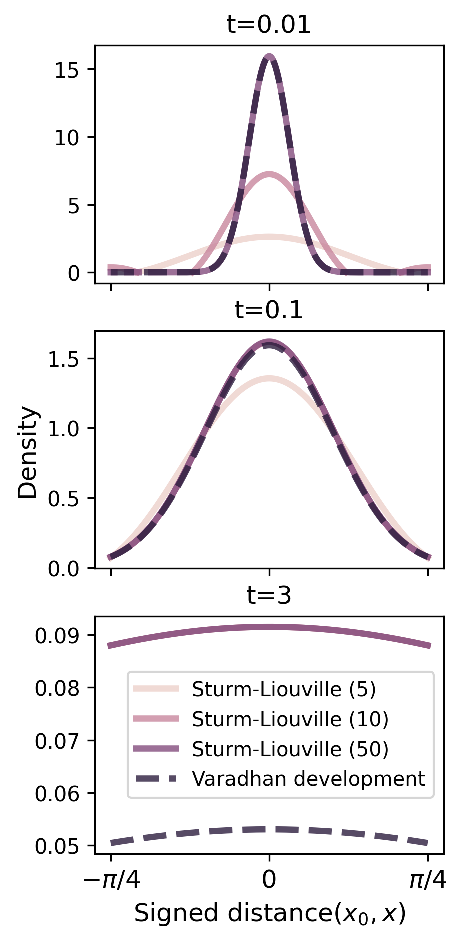
\includegraphics[width=\linewidth]{images/rsgm/s2_heat_kernel.pdf}
% 	\caption{
% 		Slice of heat kernel \(p_{t|0}(x_t|x_0)\) on \(\mathbb{S}^2\) for different approximations.
% 	}
% 	\label{fig:heat_kernel}
% \end{figure}

% We recall that in the case of compact manifolds the heat kernel is given by the Sturm--Liouville decomposition \cite{chavel1984eigenvalues} given for any \(t > 0\) and \(x, y \in \c{M}\) by \begin{equation} \label{eq:infinite_sum2} {p_{t|0}(y|x) = \sum_{j \in \N} \mathrm{e}^{-\lambda_j t} \phi_j(x)\phi_j(y),} \end{equation} where the convergence occurs in \(\mathrm{L}^2(p_{\t{ref}} \otimes p_{\t{ref}})\), \((\lambda_j)_{j \in \N}\) and \((\phi_j)_{j \in \N}\) are the eigenvalues, respectively the eigenvectors, of \(-\Delta_\c{M}\) in \(\mathrm{L}^2(p_{\t{ref}})\) \cite[see][Section 2]{saloff1994precise}.
% When the eigenvalues and eigenvectors are known, we approximate the logarithmic gradient of \(p_{t|0}\) by truncating the sum in \eqref{eq:infinite_sum2} with \(J \in \N\) terms.

% Another possibility to approximate \(\nabla \log p_{t|0}\) is to rely on the so-called Varadhan approximation, see \Cref{sec:riem-score-appr}, which is valid for small \(t >0\) .
% \Cref{fig:heat_kernel} illustrates these different
% approximations of the heat kernel and \Cref{tab:sm_losses_bis} compares the
% different loss functions.

% \begin{table}[ht]
% 	\centering
% 	\small
% 	\setlength{\tabcolsep}{0.3em}
% 	\renewcommand*{\arraystretch}{1.4}
% 	\begin{tabular}{cc|c|ccc}
% 		Loss & Approximation & Loss function & Unbiased & Consistent & Variance \\ \midrule \multirow{2}{4.5em}{\(\ell_{t|0}\) (DSM)} & Truncation~\eqref{eq:heat_kernel_trunc} & \(\frac{1}{2} \E \left[ \| s(\v{X}_t) - S_{J,t}(\v{X}_0,\v{X}_t) \|^2 \right]\) & \xmark & \cmark (\(J \rightarrow \infty\)) & 0 \\ & Varhadan~\eqref{eq:varadhan} & \(\frac{1}{2} \E \left[ \| s(\v{X}_t) - \log_{\v{X}_t}(\v{X}_0) / t \|^2 \right]\) & \xmark & \cmark (\(t \rightarrow 0\)) & 0 \\ \midrule \(\ell_{t|s}\) (DSM) & Varhadan~\eqref{eq:varadhan} & \(\frac{1}{2} \E \left[ \| s(\v{X}_t) - \log_{\v{X}_t}(\v{X}_s) / (t-s) \|^2 \right]\) & \xmark & \cmark(\(t \rightarrow s\)) & 0 \\ \midrule \multirow{2}{4.5em}{\(\ell^{\mathrm{im}}_t\) (ISM)} & Deterministic & \(\E \left[\frac{1}{2} \| s(\v{X}_t) \|^2 + \mathrm{div}( s)(\v{X}_t) \right]\) & \cmark & \cmark & 0 \\ & Stochastic & \(\E \left[\frac{1}{2} \| s(\v{X}_t) \|^2 + \varepsilon^\top \partial s(\v{X}_t) \varepsilon \right]\) & \cmark & \cmark & \(2 \| \partial s \|_F\)\\ \bottomrule\end{tabular} \caption{\small Riemannian score matching losses.
% 	}
% 	\label{tab:sm_losses_bis}
% \end{table}

% \section{Predictor-corrector schemes}
% \label{sec:predictor-corrector}

% In this section, we present a predictor-corrector scheme, adapting the techniques of \textcite{allgower2012numerical,song2020score} to the manifold setting.
% Changes between \Cref{alg:grw_rsgm}, \Cref{alg:rsgm} and \Cref{alg:grw-c}, \Cref{alg:rsgm-c} are highlighted in red.
% Let \(t \in \sbr{0,T}\), \(\gamma >0\) and \(k = \floor{t / \gamma}\).
% We remark that \Cref{alg:grw-c} (\Cref{line:dete}) corresponds to the recursion associated with \((X_j^{t,\gamma})_{j \in \N}\) such that for any \(j \in \N\) \begin{equation} X_{j+1}^{t,\gamma} = \exp_{X_j^{t,\gamma}}[\tfrac{\gamma}{2} \nabla \log p_{T-k\gamma}(X_j^{t,\gamma}) + \sqrt{\gamma} Z_{j+1}] , \end{equation} where \(\{\bar{Z}_j\}_{j \in \N}\) is a family of i.i.d Gaussian random variables with zero mean and identity covariances matrix in \(\R^p\) and for any \(j \in \N\), \(Z_j = \mathrm{P}(X_j^{t,\gamma}) \bar{Z}_j\).
% Note that here \(k \in \{0, N-1\}\) is fixed.
% Letting \(\gamma \to 0\), we obtain that under mild assumptions, see \cite[Theorem 3.1]{kuwada2012convergence}, \((X_j^{t, \gamma})_{j \in \N}\) converges to \((\v{X}_s^t)_{s \geq 0}\) such that \begin{equation} \mathrm{d} \v{X}_s^t = \tfrac{1}{2} \nabla \log p_{T-t}(\v{X}_s^t) \mathrm{d} s + \mathrm{d} \v{b}_s^\c{M} .
% \end{equation}
% We have that \(p_{T-t}\) is the invariant measure of \((\v{X}_s^t)_{s \geq 0}\).
% Hence, the role of the corrector step is to project the distribution back onto \(p_{T-t}\) for all times \(t \in \sbr{0,T}\), see \Cref{fig:illustration_pred_correc}.
% \begin{figure}[htb]
% 	\centering
% 	\begin{tikzpicture}
% 		\draw [stealth-, line width = .05cm] (0,0) .. controls  (2,-4) and (4,4) .. (6,0);
% 		\draw [-stealth, line width = .05cm, blue!50!black, dashed] (0,0) -- (1.3,-2.3);
% 		\draw [-stealth, line width = .05cm, red!50!black, dashed] (1.3,-2.3) -- (1.3,-1.2);
% 		\draw [-stealth, line width = .05cm, blue!50!black, dashed] (1.3,-1.2) -- (2.8,-0.7);
% 		\draw [-stealth, line width = .05cm, red!50!black, dashed] (2.8,-0.7) -- (2.6, -0.5);
% 		\node [below=0.2cm] at (6,0) {\(p_{\textrm{data}}\)};
% 		\node [left=0.3cm] at (0,0) {\(\mathcal{L}(X_0^\gamma) = p_T\)};
% 		\node [below=0.2cm] at (1.3,-2.3) {\(\mathcal{L}(X_{1/2}^\gamma)\)};
% 		\node [below right=0.1cm] at (1.3,-1.2) {\(\mathcal{L}(X_{1}^\gamma)\)};
% 		\node [right=0.2cm] at (2.8,-0.7) {\(\mathcal{L}(X_{3/2}^\gamma)\)};
% 		\node [above left=0.1cm] at (2.6, -0.5) {\(\mathcal{L}(X_{2}^\gamma)\)};
% 	\end{tikzpicture}
% 	\caption{Illustration of the effect of the corrector step on RSGM.
% 		The black line corresponds to the dynamics of the noising process \((p_t)_{t \in \sbr{0,T}}\).
% 		The blue dashed lines correspond to the predictor step (going backward in time) and the red dashed lines correspond to the corrector step (projecting back onto the initial dynamics).
% 		Note that \(\mathcal{L}(X_1^\gamma) \approx p_{T- \gamma}\) and \(\mathcal{L}(X_2^\gamma) \approx p_{T- 2\gamma}\).
% 	}
% 	\label{fig:illustration_pred_correc}
% \end{figure}

% \begin{algorithm}[!ht]
% 	\caption{\small GRW-c (Geodesic Random Walk with corrector)}
% 	\label{alg:grw-c}
% 	\begin{algorithmic}[1]
% 		\small
% 		\Require \(T, N, X_0^\gamma, b, \sigma, \mathrm{P}\)
% 		\State \(\gamma = T / N\) \Comment Step-size
% 		\For{\(k \in \{0, \dots, N-1\}\)}
% 		\State \textcolor{blue!50!black}{/// PREDICTOR STEP}
% 		\State \textcolor{blue!50!black}{\(\bar{Z}_{k+1/2} \sim \mathrm{N}(0, \mathrm{I}_p)\)} \Comment Standard Gaussian in ambient space \(\R^p\)
% 		\State \textcolor{blue!50!black}{\(Z_{k+1/2} = \mathrm{P}(X_k^\gamma) \bar{Z}_{k+1/2}\)} \Comment Projection in the tangent space \(\mathrm{T}_x \c{M}\)
% 		\State \textcolor{blue!50!black}{\(W_{k+1/2} = \gamma b(k \gamma, X_k^\gamma) + \sqrt{\gamma} \sigma(k \gamma, X_k^\gamma) Z_{k+1/2}\)} \Comment Euler--Maruyama step on tangent space
% 		\State \textcolor{blue!50!black}{\(X_{k+1/2}^\gamma = \exp_{X_k^\gamma}[W_{k+1/2}]\)} \Comment Geodesic projection onto \(\c{M}\)
% 		\State \textcolor{red!50!black}{/// CORRECTOR STEP}
% 		\State \textcolor{red!50!black}{\(\bar{Z}_{k+1} \sim \mathrm{N}(0, \mathrm{I}_p)\)} \Comment Standard Gaussian in ambient space \(\R^p\)
% 		\State \textcolor{red!50!black}{\(Z_{k+1} = \mathrm{P}(X_{k+1/2}^\gamma) \bar{Z}_{k+1}\)} \Comment Projection in the tangent space \(\mathrm{T}_x \c{M}\)
% 		\State \textcolor{red!50!black}{\(W_{k+1} = \tfrac{\gamma}{2} b(k \gamma, X_{k+1/2}^\gamma) + \sqrt{\gamma} \sigma(k \gamma, X_{k+1/2}^\gamma) Z_{k+1}\)} \Comment Euler--Maruyama step on tangent space \label{line:dete}
% 		\State \textcolor{red!50!black}{\(X_{k+1}^\gamma = \exp_{X_{k+1/2}^\gamma}[W_{k+1}]\)} \Comment Geodesic projection onto \(\c{M}\)
% 		\EndFor
% 		\State {\bfseries return} \(\{ X_k^\gamma\}_{k=0}^{N}\)
% 	\end{algorithmic}
% \end{algorithm}

% \begin{algorithm}[!t]
% 	\caption{\small RSGM-c (Riemannian Score-Based Generative Model with corrector)}
% 	\label{alg:rsgm-c}
% 	\begin{algorithmic}[1]
% 		\small
% 		\Require \(\varepsilon, T, N, \{X_0^m\}_{m=1}^M, \mathrm{loss}, \mathbf{s}, \theta_0, N_{\textrm{iter}}, p_{\t{ref}}, \mathrm{P}\)
% 		\State{{/// TRAINING ///}}

% 		\For{\(n \in \{0, \dots, N_{\textrm{iter}}-1\}\)}
% 		\State \(X_0 \sim (1/M) \sum_{m=1}^M \delta_{X_0^m}\) \Comment Random mini-batch from dataset
% 		\State \(t \sim U(\sbr{\varepsilon, T})\) \Comment Uniform sampling between \(\varepsilon\) and \(T\)
% 		\State \(\v{X}_t = \textrm{GRW}(t, N, X_0, 0, \m{I}, \mathrm{P})\) \Comment Approximate forward diffusion with \cref{alg:grw_rsgm}

% 		\State
% 		\(\ell(\theta_n) = \ell_t(T, N, X_0, \v{X}_t, \mathrm{loss}, \mathbf{s}_{\theta_n})\)
% 		\Comment Compute score matching loss from \cref{tab:sm_losses} \State
% 		\(\theta_{n+1} = \verb|optimizer_update|(\theta_n, \ell(\theta_n))\) \Comment ADAM
% 		optimizer step
% 		\EndFor \State \(\theta^\star = \theta_{N_{\textrm{epoch}}}\)
% 		\State{{/// SAMPLING ///}} \State \(Y_0 \sim p_{\t{ref}}\) \Comment
% 		Sample from uniform distribution \State
% 		\(b_\theta^\star(t, x) = \mathbf{s}_{\theta^\star}(T-t, x)\) for any
% 		\(t \in \sbr{0,T}\), \(x \in \c{M}\) \Comment Reverse process drift \State
% 		$\{Y_k\}_{k=0}^{N} = \textrm{GRW-c}(T, N, Y_0, b_{\theta^\star}, \m{I},
% 			\mathrm{P})$ \Comment Approximate reverse diffusion with \Cref{alg:grw-c} \State
% 		{\bfseries return} \(\theta^\star, \{Y_k\}_{k=0}^{N}\)
% 	\end{algorithmic}
% \end{algorithm}

\section{Time-reversal formula: extension to  Riemannian manifolds}
\label{sec:time-reversal-manifold-proof}

In this section, we provide the proof of \Cref{thm:time_reversal_manifold}.
The proof follows the arguments of \textcite[Theorem 4.9]{cattiaux2021time}.
We could have also applied the abstract results of \textcite[Theorem 5.7]{cattiaux2021time} to obtain our results.
Note that the time-reversal on manifold could also be obtained by readily extending arguments from \textcite{haussmann1986time}, however the entropic conditions found by \textcite{cattiaux2021time} are more natural when it comes to the study of the Schr\"odinger Bridge problem.
For the interested reader we provide an informal derivation of the time-reversal formula obtained by \textcite{haussmann1986time} in \cref{sec:informal-derivation}.
The proof of \Cref{thm:time_reversal_manifold} is given in \cref{sec:proof-crefthm:t}.
Finally, we emphasize that \textcite{garcia2021brenier} have developed a Girsanov theory for stochastic processes defined on compact manifolds with boundary in order to study the Brenier-Schr\"odinger problem.

\subsection{Informal derivation}
\label{sec:informal-derivation}

In this section, we provide a non-rigorous derivation of \Cref{thm:time_reversal_manifold} following the approach of \textcite{haussmann1986time}.
Let \((\v{X}_t)_{t \in \sbr{0,T}}\) be a continuous process such that for any \(f \in \mathrm{C}^2(\c{M})\) we have that \((\v{M}_t^{\v{X}, f})_{t \in \sbr{0,T}}\) is a \(\v{X}\)-martingale where for any \(t \in \sbr{0,T}\) \begin{equation} \label{eq:martingale_forward} { \v{M}_t^{\v{X}, f} = f(\v{X}_t) - \int_0^t \{ \langle b(\v{X}_s), \nabla f(\v{X}_s) \rangle + \tfrac{1}{2} \Delta_\c{M} f(\v{X}_s) \} \mathrm{d} s .
	}
\end{equation}
Let \((\v{Y}_t)_{t \in \sbr{0,T}} = (\v{X}_{T-t})_{t \in \sbr{0,T}}\).
Our goal is to show that for any \(f \in \mathrm{C}^2(\c{M})\), \((\v{M}_t^{\v{Y}, f})_{t \in \sbr{0,T}}\) is a \(\v{Y}\)-martingale where for any \(t \in \sbr{0,T}\) \begin{equation} { \v{M}_t^{\v{Y}, f} = f(\v{Y}_t) - \int_0^t \{ \langle - b(\v{Y}_s) + \nabla \log p_{T-s}(\v{Y}_s), \nabla f(\v{Y}_s) \rangle + \tfrac{1}{2} \Delta_\c{M} f(\v{Y}_s) \} \mathrm{d} s .
	}
\end{equation}
Note that here we implicitly assume that for any \(t \in \sbr{0,T}\), \(\v{X}_t\) admits a smooth positive density with respect to.
\(p_{\t{ref}}\) denoted \(p_t\).
In other words, we want to show that for any \(g \in \mathrm{C}^2(\c{M})\) and \(s, t \in \sbr{0,T}\) with \(t \geq s\) we have \begin{align} \label{eq:time_reversal_manifold_haussman} & {\E\sbr{g(\v{Y}_s)(f(\v{Y}_t) - f(\v{Y}_s))}} \\  & \qquad {= \E\sbr{g(\v{Y}_s)\int_s^t \{ \langle - b(\v{Y}_u) + \nabla \log p_{T-u}(\v{Y}_u), \nabla f(\v{Y}_u) \rangle + \tfrac{1}{2} \Delta_\c{M} f(\v{Y}_u) \} \mathrm{d} u} .
                 }
\end{align}
We introduce the infinitesimal generator \(\c{A}: \ \mathrm{C}^2(\c{M}) \to \mathrm{C}(\c{M})\) given for any \(f \in \mathrm{C}^2(\c{M})\) and \(x \in \c{M}\) by \begin{equation} \c{A} (f)(x) = \langle b(x) , \nabla f(x) \rangle + \tfrac{1}{2} \Delta_\c{M} f(x) .
\end{equation}
Similarly, we introduce the infinitesimal generator \(\c{A}t: \ \sbr{0,T} \times \mathrm{C}^2(\c{M}) \to \mathrm{C}(\c{M})\) given for any \(f \in \mathrm{C}^2(\c{M})\), \(t \in \sbr{0,T}\) and \(x \in \c{M}\) by \begin{equation} \c{A}t (t, f)(x) = \langle -b(x) + \nabla \log p_{T-t}(x), \nabla f(x) \rangle + \tfrac{1}{2} \Delta_\c{M} f(x) .
\end{equation}
With these notations, \eqref{eq:time_reversal_manifold_haussman1} can be written as follows: we want to show that for any \(g \in \mathrm{C}^2(\c{M})\) and \(s, t \in \sbr{0,T}\) with \(t \geq s\) we have \begin{equation} \label{eq:time_reversal_manifold_haussman1} {\E\sbr{g(\v{Y}_s)(f(\v{Y}_t) - f(\v{Y}_s))} = \E\sbr{g(\v{Y}_s)\int_s^t \c{A}t(u, \v{Y}_u) \mathrm{d} u} .
	}
\end{equation}
The rest of this section follows the first part of the proof of \textcite[Theorem 2.1]{haussmann1986time}.
Let \(t, s \in \sbr{0,T}\) with \(t \geq s\).
We have \begin{align} \E&\sbr{g(\v{Y}_s)(f(\v{Y}_t) - f(\v{Y}_s))}\\ &= {\E\sbr{g(\v{X}_{T-s})(f(\v{X}_{T-t}) - f(\v{X}_{T-t}))}} \\ &= {\E\sbr{\E\sbrvert{g(\v{X}_{T-s})}{\v{X}_{T-t}}f(\v{X}_{T-t})} - \E\sbr{g(\v{X}_{T-s})f(\v{X}_{T-s})}} \\ &= {\E\sbr{v(T-t,\v{X}_{T-t})f(\v{X}_{T-t})} - \E\sbr{v(T-s,\v{X}_{T-s})f(\v{X}_{T-s})}} , \label{eq:first_der} \end{align} with \(v: \ \sbr{0,T-s} \times \c{M} \to \R\) given for any \(u \in \sbr{0,T-s}\) and \(x \in \c{M}\) by \(v(u,x) = \E\sbrvert{g(\v{X}_{T-s})}{\v{X}_u=x}\).
We have that \(v\) satisfies the backward Kolmogorov equation, i.e. we have for any \(u \in \sbr{0,T-s}\) and \(x \in \c{M}\) \begin{equation} \label{eq:backward_kolmogorov} \partial_u v(u,x) = -\c{A} v(u,x) .
\end{equation}
Note that it is not trivial to show that \(v\) is regular enough to satisfy the backward Kolmogorov equation.
In this informal derivation, we assume that \(v\) is regular enough and will provide a different rigorous proof of the time-reversal formula in \cref{sec:proof-crefthm:t}.
However, note that it is possible to show that \(v\) indeed satisfies the backward Kolmogorov equation by adapting arguments from \textcite{haussmann1986time} to the manifold framework.

Let \(h: \ \sbr{0,T-s} \times \c{M} \to \R\) given for any \(u \in \sbr{0,T-s}\) and \(x \in \c{M}\) by \(h(u,x) = v(u,x) f(x)\).
Using \eqref{eq:backward_kolmogorov}, we have for any \(u \in \sbr{0,T-s}\) and \(x \in \c{M}\) \begin{align} \partial_u& h(u,x) + \c{A} h(u, x)\\ & = f(x) \partial_u v(u,x) + f(x) \c{A} v(u,x) + v(u,x) \c{A} f(x) + \langle \nabla f(x), \nabla v(u,x)\rangle \\  & = v(u,x) \c{A} f(x) + \langle \nabla f(x), \nabla v(u,x)\rangle .
                 \label{eq:def_h}
\end{align}
In addition, using the divergence theorem \parencite[see][p.51]{lee2018introduction}, we have for any \(u \in \sbr{0,T-s}\) \begin{align}  & \E\sbr{\langle \nabla f(\v{X}_u), \nabla v(u,\v{X}_u)\rangle} = {\int_{\c{M}} \langle \nabla f(x_u), \nabla v(u,x_u) p_u(x_u) \rangle \mathrm{d} p_{\t{ref}}(x_u) } \\ & \qquad \qquad = - {\int_{\c{M}} v(u,x_u) \mathrm{div}(p_u \nabla f) (x_u) \mathrm{d} p_{\t{ref}}(x_u) } \\ & \qquad \qquad = - {\int_{\c{M}} v(u,x_u) \Delta_\c{M} f(x_u) p_u(x_u) \mathrm{d} p_{\t{ref}}(x_u)} \\ & \qquad \qquad \qquad {- \int_{\c{M}} v(u,x_u) \langle \nabla f(x_u), \nabla \log p_u(x_u) \rangle p_u(x_u) \mathrm{d} p_{\t{ref}}(x_u) } \\ & \qquad \qquad = - {\E\sbr{ v(u,\v{X}_u) \Delta_\c{M} f(\v{X}_u)} - \E\sbr{ v(u,\v{X}_u) \langle \nabla f(\v{X}_u), \nabla \log p_u(\v{X}_u) \rangle} } .
\end{align}
Therefore, using this result and \eqref{eq:def_h} we get that for any \(u \in \sbr{0,T-s}\) \begin{align}  & \E\sbr{\partial_u h(u,\v{X}_u) + \c{A} h(u, \v{X}_u)} \\ &= \E\sbr{v(u,\v{X}_u)\{ \langle b(\v{X}_u) - \nabla \log p_u(\v{X}_u), \nabla f(\v{X}_u) \rangle -\tfrac{1}{2} \Delta_\c{M} f(\v{X}_u)\}} \\ &= -\E\sbr{v(u,\v{X}_u)\c{A}t(T-u,f)(\v{X}_u)} .
\end{align}
Combining this result and \eqref{eq:martingale_forward} and that for any \(u \in \sbr{0,T-s}\) and \(x \in \c{M}\), \(v(u,x) = \E\sbrvert{g(\v{X}_{T-s})}{\v{X}_u=x}\) we get \begin{align}  & \E\sbr{v(T-t,\v{X}_{T-t})f(\v{X}_{T-t})} - \E\sbr{v(T-s,\v{X}_{T-s})f(\v{X}_{T-s})} \\ & \qquad \qquad \qquad = \E\sbr{h(T-t, \v{X}_{T-t}) - h(T-s, \v{X}_{T-s})} \\ & \qquad \qquad \qquad = {\int_{T-t}^{T-s} \E\sbr{v(u,\v{X}_u)\c{A}t(T-u, \v{X}_u)} \mathrm{d} u } \\  & \qquad \qquad \qquad= {\E\sbr{g(\v{X}_{T-s})\int_{T-t}^{T-s} \c{A}t(T-u, \v{X}_u) \mathrm{d} u } .
              }
\end{align}
Using this result, \eqref{eq:first_der} and the change of variable \(u \mapsto T-u\) we obtain \begin{align} \E\sbr{g(\v{Y}_s)(f(\v{Y}_t) - f(\v{Y}_s))} &= {\E\sbr{g(\v{X}_{T-s})\int_{T-t}^{T-s} \c{A}t(T-u, \v{X}_u) \mathrm{d} u } } \\ &= {\E\sbr{g(\v{Y}_{s})\int_{s}^{t} \c{A}t(u, \v{Y}_u) \mathrm{d} u } } .
\end{align}
Hence, \eqref{eq:time_reversal_manifold_haussman} holds and we have proved \Cref{thm:time_reversal_manifold}.
Again, we emphasize that in order to make the proof completely rigourous one needs to derive regularity properties of \(v\).

\subsection{Proof of \Cref{thm:time_reversal_manifold}}
\label{sec:proof-crefthm:t}

In this section, we follow another approach to prove the time-reversal formula.
We are going to use the integration by part formula of \textcite[Theorem 3.17]{cattiaux2021time} in a similar spirit as \textcite[Theorem 4.9]{cattiaux2021time} in the Euclidean setting.
In order to adapt arguments from \textcite{cattiaux2021time} to our Riemannian setting, we use the Nash embedding theorem in order to embed our processes in a Euclidean space and leverage tools from Girsanov theory.
The rest of the section is organized as follows.
First in \cref{sec:diff-proc-stoch}, we recall basic properties of infinitesimal generators and recall the integration by part formula of \textcite[Theorem 3.17]{cattiaux2021time}.
Then in \cref{sec:girs-theory-comp}, we extend some Girsanov theory to compact Riemannian manifolds using the Nash embedding theorem.
We conclude the proof in \cref{sec:concluding-proof}.

\subsubsection{Diffusion processes and integration by part formula}
\label{sec:diff-proc-stoch}

In this section, we state a simplified version of \textcite[Theorem 3.17]{cattiaux2021time} for Markov continuous path (probability) measure on Polish spaces.
Let \((\sf{X}, \c{X})\) be a Polish space.
We say that \(\bb{P}\) is a path measure if \(\bb{P} \in \c{P}(\mathrm{C}(\sbr{0,T}, \sf{X}))\).
Let \((\v{X}_t)_{t \in \sbr{0,T}}\) with distribution \(\bb{P}\).
We denote \((\c{F}_t)_{t \in \sbr{0,T}}\) the filtration such that for any \(t \in \sbr{0,T}\), \(\c{F}_t = \sigma(\v{X}_s, \ s \in \sbr{0,t})\).
Let \((\v{M}_t)_{t \in \sbr{0,T}}\) be a Polish-valued stochastic process.
We say that \((\v{M}_t)_{t \in \sbr{0,T}}\) is a \(\bb{P}\)-local martingale if it is a local martingale with respect to.
the filtration \((\c{F}_t)_{t \in \sbr{0,T}}\).
A function \(u: \sbr{0,T} \times \sf{X} \to \R\) is said to be in the domain of the extended generator of \(\bb{P}\) if there exists a process \((\c{A} b_{\bb{P}} u(t, \v{X}_{\sbr{0,t}}))_{t \in \sbr{0,T}}\) such that: \begin{enumerate}[label= (\alph*), wide, labelindent=0pt] \item \((\c{A}b_{\bb{P}} u(t, \v{X}_{\sbr{0,t}}))_{t \in \sbr{0,T}}\) is adapted with respect to.
	      \((\c{F}_t)_{t \in \sbr{0,T}}\).
	\item \(\int_0^T \abs{\c{A}b_{\bb{P}} u(t, \v{X}_{\sbr{0,t}})} \mathrm{d} t < +\infty\), \(\bb{P}\)-a.s.
	\item The process \((\v{M}_t)_{t \in \sbr{0,T}}\) is a \(\bb{P}\)-local martingale,
	      where for any \(t \in \sbr{0,T}\)
	      \begin{equation}
		      {\v{M}_t = u(t,\v{X}_t) - u(0, \v{X}_0) - \int_0^t \c{A}b_{\bb{P}} u(s, \v{X}_{\sbr{0,s}}) \mathrm{d} s   .}
	      \end{equation}
\end{enumerate}
The domain of the extended generator is denoted \(\rm{dom}(\c{A}b_{\bb{P}})\).
We say that \((u,v)\) with \(u,v : \ \sbr{0,T} \times \sf{X} \to \R\) is in the domain of the carr\'e du champ if \(u,v, uv \in \rm{dom}(\c{A}b_{\bb{P}})\).
In this case, we define the carr\'e du champ \(\bar{\carrechamp}_{\bb{P}}\) as \begin{equation} \bar{\carrechamp}_{\bb{P}}(u,v) = \c{A}b_{\bb{P}}(uv) - \c{A}b_{\bb{P}}(u)v - \c{A}b_{\bb{P}}(v)u .
\end{equation}
Note that if \(\sf{X} = \c{M}\) is a Riemannian manifold, \(\mathrm{C}^2(\c{M}) \subset \rm{dom}(\c{A}b_{\bb{P}})\) and for any \(u \in \mathrm{C}^2(\c{M})\) \(\c{A}b_{\bb{P}}(u) = \langle \nabla u, X \rangle + \tfrac{1}{2}\Delta_\c{M} u\) with \(X \in \Gamma(\TM)\) then we have that \(\mathrm{C}^2(\c{M}) \times \mathrm{C}^2(\c{M}) \subset \rm{dom}(\bar{\carrechamp}_{\bb{P}})\) and for any \(u, v \in \mathrm{C}^2(\c{M})\), \(\bar{\carrechamp}_{\bb{P}}(u,v) = \langle \nabla u, \nabla v \rangle\).
Assume that there exists \(\mathcal{U}_{\bb{P}} \subset \rm{dom}(\c{A}b_{\bb{P}}) \cap \mathrm{C}_b(\sf{X})\) such that \(\mathcal{U}_{\bb{P}}\) is an algebra.
We denote \(\mathcal{U}_{\bb{P},2}\) such that \begin{equation} \mathcal{U}_{\bb{P},2} = \cbrcolon{u \in \mathcal{U}_{\bb{P}}}{\c{A}b_{\bb{P}} u \in \mathrm{L}^2(\bb{P}), \ \bar{\carrechamp}_{\bb{P}}(u,u) \in \mathrm{L}^1(\bb{P})} .
\end{equation}
Finally we denote \(R(\bb{P})\) the time-reverse path measure, i.e. for any \(\mathsf{A} \in \c{b}\del{\mathrm{C}(\sbr{0,T}, \sf{X})}\) we have \(R(\bb{P})(\mathsf{A}) = \bb{P}(R(\mathsf{A}))\), where \(R(\mathsf{A}) = \cbrcolon{t \mapsto \omega_{T-t}}{\omega \in \mathsf{A}}\).
In what follows, we assume \(\bb{P}\) is Markov.
It is well-known, see \parencite[Theorem 1.2]{leonard2014reciprocal} for instance, that in this case \(R(\bb{P})\) is also Markov.
In addition, since \(\bb{P}\) is Markov, for any \(u \in \mathrm{dom}(\c{A}b_{\bb{P}})\) and \(t \in \sbr{0,T}\) there exists \(\c{A}_{\bb{P}}\) such that \(\c{A}b_{\bb{P}} u(t, \v{X}_{\sbr{0,t}}) = \c{A}_{\bb{P}} u(t, \v{X}_t)\) with \(\c{A}_{\bb{P}} u: \ \sbr{0,T} \times \sf{X} \to \R\).
Similarly, we define \(\carrechamp_{\bb{P}}(u,v): \ \sbr{0,T} \times \sf{X} \to \R\) from \(\bar{\carrechamp}_{\bb{P}}(u,v)\).

We are now ready to state the integration by part formula, \parencite[Theorem 3.17]{cattiaux2021time}.

\begin{theorem}
	\label{thm:ibp_cattiaux}
	Let \(u, v \in \mathcal{U}_{\bb{P}, 2}\).
	The following hold: \begin{enumerate}[label= (\alph*), wide, labelindent=0pt] \item If \(u \in \rm{dom}(\c{A}_{R(\bb{P})})\) and \(\c{A}_{R(\bb{P})}u \in \mathrm{L}^1(\bb{P})\) then for almost any \(t \in \sbr{0,T}\) \begin{equation} \E\sbr{\{\c{A}_{\bb{P}} u(t, \v{X}_t) + \c{A}_{R(\bb{P})} u (T-t, \v{X}_t)\}v(\v{X}_t) + \carrechamp_{\bb{P}}(u,u)(t, \v{X}_t)} = 0 .
		      \end{equation}
		\item If the following hold:
		      \begin{enumerate}[label=\roman*)]
			      \item \(\carrechamp_{\bb{P}}(u,v) \in \mathrm{C}(\sbr{0,T} \times \sf{X}, \R)\).
			      \item \(\mathcal{U}_{2, \bb{P}}\) determines the weak convergence of Borel measures.
			      \item \(\mu\) defines a finite measure on \(\sbr{0,T} \times \sf{X}\) where for
			            any \(\omega \in \bar{\mathcal{U}}_{2, \bb{P}}\) we have
			            \begin{equation}
				            {\mu[\omega] = \E\sbr{\int_0^T \carrechamp_{\bb{P}}(u,\omega_t)(t, \v{X}_t) \mathrm{d} t }},
			            \end{equation}
			            where
			            $\bar{\mathcal{U}}_{2, \bb{P}} = \cbrcolon{\omega \in \mathrm{C}(\sbr{0,T}
				            \times \sf{X}, \R)}{\omega(t, \cdot) \in \mathcal{U}_{2, \bb{P}}\ \
				            \text{for any \(t \in \sbr{0,T}\)}}$.
		      \end{enumerate}
		      Then \(u \in \rm{dom}(\c{A}_{R(\bb{P})})\) and \(\c{A}_{R(\bb{P})}u \in \mathrm{L}^1(\bb{P})\).
	\end{enumerate}
\end{theorem}

Note that this theorem is a simplified version of \textcite[Theorem 3.17]{cattiaux2021time} where we restrict ourselves to the case of Markov path measures.
In what follows, we wish to apply \Cref{thm:ibp_cattiaux} to diffusion processes on manifolds.
To do so, we will verify that under a finite entropy assumption, the conditions \(u \in \rm{dom}(\c{A}_{R(\bb{P})})\) and \(\c{A}_{R(\bb{P})}u \in \mathrm{L}^1(\bb{P})\) are fullfilled for a class of regular functions \(u\).
These integrability results are obtained using Girsanov theory.

\subsubsection{Girsanov theory on compact Riemannian manifolds}
\label{sec:girs-theory-comp}

In this section, we will consider two types of martingale problems: one on Euclidean spaces and one on the compact Riemannian manifold \(\c{M}\).
Let \(\bb{P} \in \c{P}(\mathrm{C}(\sbr{0,T}, \R^p))\).
We say that \(\bb{P}\) satisfies the (Euclidean) martingale problem with infinitesimal generator \(\c{A}: \ \sbr{0,T} \times \mathrm{C}^2(\R^p) \times \R^p \to \R\) if for any \(u \in \mathrm{C}_c^2(\R^p)\), \((\v{M}_t)_{t \in \sbr{0,T}}\) is a \(\bb{P}\)-martingale where for any \(t \in \sbr{0,T}\) we have \begin{equation} { \v{M}_t = \v{M}_0 + \int_0^t \c{A}(t, u)(\v{X}_s) \mathrm{d} s , } \end{equation} where \((\v{X}_t)_{t \in \sbr{0,T}}\) has distribution \(\bb{P}\) and \(\int_0^T \abs{\c{A}(t, u)(\v{X}_s) \mathrm{d} t} <+\infty\), \(\bb{P}\)-a.s.
Let \(\bb{P} \in \c{P}(\mathrm{C}(\sbr{0,T}, \c{M}))\).
We say that \(\bb{P}\) satisfies the (Riemannian) martingale problem with infinitesimal generator \(\c{A}t: \ \sbr{0,T} \times \mathrm{C}^2(\c{M}) \times \c{M} \to \R\) if for any \(u \in \mathrm{C}^2(\c{M})\), \((\v{M}_t)_{t \in \sbr{0,T}}\) is a \(\bb{P}\)-martingale where for any \(t \in \sbr{0,T}\) we have \begin{equation} { \v{M}_t = \v{M}_0 + \int_0^t \c{A}t(t, u)(\v{X}_s) \mathrm{d} s , } \end{equation} where \((\v{X}_t)_{t \in \sbr{0,T}}\) has distribution \(\bb{P}\) and \(\int_0^T \abs{\c{A}t(t, u)(\v{X}_s) \mathrm{d} t} <+\infty\), \(\bb{P}\)-a.s.
We now prove the following theorem.

\begin{proposition}[Girsanov Theroy on Manifolds]
	\label{prop:girsanov_manifold}
	Let \(\bb{Q}\) be the path measure of a Brownian motion on \(\c{M}\).
	Let \(\bb{P}\) be a Markov path measure on \(\mathrm{C}(\sbr{0,T}, \c{M})\) such that \(\f{KL}\delvert{\bb{P}}{\bb{Q}} < +\infty\).
	Then there exists \(\beta\) such that for any \(t \in \sbr{0,T}\) and \(x \in \c{M}\), \(\beta(t,x) \in \mathrm{T}_x \c{M}\) and we have that \(\bb{P}\) satisfies the martingale problem with infinitesimal generator \(\c{A}\) where for any \(t \in \sbr{0,T}\), \(u \in \mathrm{C}^2(\c{M})\) and \(x \in \c{M}\) we have \begin{equation} \c{A}(t,u)(x) = \langle \beta(t,x), \nabla u(x) \rangle + \tfrac{1}{2} \Delta_\c{M} u(x) .
	\end{equation}
	In addition, we have that \begin{equation} {\f{KL}\delvert{\bb{P}}{\bb{Q}} = \f{KL}\delvert{\bb{P}_0}{\bb{Q}_0} + \tfrac{1}{2} \int_0^T \E\sbr{\norm{\beta(t, \v{X}_t)}^2} \mathrm{d} t ,} \end{equation} where \((\v{X}_t)_{t \in \sbr{0,T}}\) has distribution \(\bb{P}\).
\end{proposition}

\begin{proof}
	First, we extend \((\v{b}_t^\c{M})_{t \in \sbr{0,T}}\) to \(\R^p\) using the Nash embedding theorem \parencite[see][]{gunther1991isometric}.
	\((\v{b}_t^\c{M})_{t \in \sbr{0,T}}\) can be seen as a process on \(\R^p\) (for
	some \(p \in \N\)) which satisfies in a weak sense
	\begin{equation}
		{
			\mathrm{d} \v{b}_t^\c{M} = \sum_{i=1}^p \mathrm{P}_i(\v{b}_t^\c{M}) \circ \mathrm{d} \v{b}_t^i  = P(\v{b}_t^\c{M}) \circ \mathrm{d} \v{b}_t  ,
		}
	\end{equation}
	where \((\v{b}_t)_{t \in \sbr{0,T}}\) is a \(p\)-dimensional Brownian motion
	and \(\mathrm{P} \in \mathrm{C}^\infty(\R^p, \R^{p\times p})\) is such that for any
	\(x \in \c{M}\), \(\mathrm{P}(x)\) is the projection onto \(\mathrm{T}_x \c{M}\) and for any
	\(i \in \{1, \dots, p\}\), \(\mathrm{P}_i \in \mathrm{C}^\infty(\R^p, \R^p)\) with
	\(\mathrm{P}_i = \mathrm{P} e_i\) where \(\{e_j\}_{j=1}^p\) is the canonical basis of
	\(\R^p\).
	We refer to \Cref{sec:metr-conn-tens} for more details on the projection operator and its extension to \(\R^p\).
	Using the link between Stratanovitch and It\^o integral, there exists \(\bar{b} \in \mathrm{C}^\infty(\R^p, \R^p)\) such that \((\v{b}_t^\c{M})_{t \in \sbr{0,T}}\) can be seen as a process on \(\R^p\) which satisfies in a weak sense \begin{equation} { \mathrm{d} \v{b}_t^\c{M} = \bar{b}(\v{b}_t^\c{M}) \mathrm{d} t + \mathrm{P}(\v{b}_t^\c{M}) \mathrm{d} \v{b}_t , } \end{equation} where \(\bar{b}\) is given in \eqref{eq:strata_ito_transfo_sde} and satisfies \(\mathrm{P}\bar{b}(x) = 0\) for any \(x \in \c{M}\), see the remark following \eqref{eq:strata_ito_transfo_sde}.
	For any \(u, v \in \mathrm{C}^2_c(\c{M})\), we consider \(\bar{u}, \bar{v}\) extensions to \(\mathrm{C}^2_c(\R^p)\) and we have for any \(s, t \in \sbr{0,T}\) \begin{align}  & {\E\sbr{\bar{v}(\v{b}_s^\c{M}) \int_s^t \tfrac{1}{2} \Delta_\c{M} u(\v{b}_u^\c{M}) \mathrm{d} u}} \\  & \qquad = {\E\sbr{\bar{v}(\v{b}_s^\c{M}) \int_s^t \{ \langle \nabla \bar{u}(\v{b}_w^\c{M}), \bar{b}(\v{b}_w^\c{M}) \rangle + \tfrac{1}{2} \langle \mathrm{P}(\v{b}_w^\c{M}), \nabla^2 \bar{u}(\v{b}_w^\c{M}) \rangle \} \mathrm{d} w} .
                 }
	\end{align}
	In particular, we get that for any \(x \in \c{M}\), \(\Delta_\c{M} u(x) = 2 \langle \nabla \bar{u}(x), \bar{b}(x) \rangle + \langle \mathrm{P}(x), \nabla^2 \bar{u}(x) \rangle\).
	Note that \((\v{b}_t^\c{M})_{t \in \sbr{0,T}}\) (seen as a process on \(\R^p\)) satisfies the condition \(\mathrm{(U)}\) in \textcite{leonard2012girsanov}, i.e. uniqueness of the trajectories given an initial condition.
	Therefore applying \cite[Theorem 2.1]{leonard2012girsanov}, \parencite[Claim 4.5]{cattiaux2021time}, there exists \(\bar{\beta}: \ \sbr{0,T} \times \R^p \to \R^p\) such that \begin{equation} \label{eq:KL_ineq1} {\f{KL}\delvert{\bb{P}}{\bb{Q}} = \f{KL}\delvert{\bb{P}_0}{\bb{Q}_0} + \tfrac{1}{2} \int_0^T \E\sbr{\norm{\mathrm{P}(\v{X}_t) \bar{\beta}(t, \v{X}_t)}^2} \mathrm{d} t .
		}
	\end{equation}
	In addition, \(\bb{P}\) (seen as a process on \(\R^p\)) satisfies a martingale problem with infinitesimal generator \(\c{A}b: \ \sbr{0,T} \times \mathrm{C}^2_c(\R^p) \times \R^p \to \R\) such that for any \(t \in \sbr{0,T}\), \(\bar{u} \in \mathrm{C}^2_c(\R^p)\) and \(x \in \R^p\) \begin{equation} \c{A}b(t,\bar{u})(x) = \langle \bar{b}(x) + \mathrm{P}(x)\bar{\beta}(t,x), \nabla \bar{u}(x) \rangle + \tfrac{1}{2} \langle \mathrm{P}(x), \nabla^2 \bar{u}(x)\rangle .
	\end{equation}
	Let \(\beta: \ \sbr{0,T} \times \c{M}\) such that for any \(t \in \sbr{0,T}\) and \(x \in \c{M}\) we have \(\beta(t,x) = \mathrm{P}(x) \bar{\beta}(t,x)\).
	In particular, we have that for any \(x \in \c{M}\), \(\beta(t,x) \in \mathrm{T}_x\c{M}\).
	Let \(u \in \mathrm{C}^2_c(\c{M})\) and consider an extension \(\bar{u}\) to \(\mathrm{C}^2_c(\R^p)\).
	For any \(t \in \sbr{0,T}\) and \(x \in \c{M}\) we have \begin{align} \c{A}b(t,\bar{u})(x) & = \langle \bar{b}(x) + \mathrm{P}(x)\bar{\beta}(t,x), \nabla \bar{u}(x) \rangle + \tfrac{1}{2} \langle \mathrm{P}(x), \nabla^2 \bar{u}(x)\rangle \\ &= \langle \beta(t,x), \nabla \bar{u}(x) \rangle + \tfrac{1}{2} \Delta_\c{M} u(x) \\ &=\langle \beta(t,x), \nabla u(x) \rangle + \tfrac{1}{2} \Delta_\c{M} u(x) .
	\end{align}
	In particular, we have that \(\bb{P}\) (seen as a process on \(\c{M}\)) satisfies a martingale problem with infinitesimal generator \(\c{A}: \ \sbr{0,T} \times \mathrm{C}^2_c(\c{M}) \times \c{M} \to \R\) such that for any \(t \in \sbr{0,T}\), \(u \in \mathrm{C}^2(\R^p)\) and \(x \in \c{M}\) \begin{equation} \c{A}(t,\bar{u})(x) = \langle \beta(t,x), \nabla u(x) \rangle + \tfrac{1}{2} \Delta_\c{M} u(x) .
	\end{equation}
	In addition, rewriting \eqref{eq:KL_ineq1} we have \begin{equation} \label{eq:KL_ineq} {\f{KL}\delvert{\bb{P}}{\bb{Q}} = \f{KL}\delvert{\bb{P}_0}{\bb{Q}_0} + \tfrac{1}{2} \int_0^T \E\sbr{\norm{\beta(t, \v{X}_t)}^2} \mathrm{d} t ,} \end{equation} which concludes the proof.
\end{proof}

We also derive the following useful lemma, which will be used in the proof of convergence of RSGM.

\begin{corollary}
	\label{col:KL_diff}
	Assume \Cref{assum:manifold}.
	Let \(\bb{P}^1, \bb{P}^2\) be a Markov path measure on \(\mathrm{C}(\sbr{0,T}, \c{M})\) with \(\bb{P}_0^1 = \bb{P}_0^2\).
	In addition, assume that there exist \(b_1,b_2 \in \mathrm{C}^\infty(\sbr{0,T}, \c{X}(\c{M}))\) such that \((\v{X}_t^1)_{t \in \sbr{0,T}}\) and \((\v{X}_t^2)_{t \in \sbr{0,T}}\) are associated to \(\bb{P}^1\) and \(\bb{P}^2\) respectively and satisfy weakly \(\mathrm{d} \v{X}_t^i = b_1(t,\v{X}_t^i) \mathrm{d} t + \mathrm{d} \v{b}_t\) for \(i \in \{1,2\}\).
	Then, we have that \begin{equation} {\f{KL}\delvert{\bb{P}^1}{\bb{P}^2} = \tfrac{1}{2} \int_0^T \E\sbr{\norm{b_1(t,\v{X}_t^1) - b_2(t,\v{X}_t^1)}^2} \mathrm{d} t .
		}
	\end{equation}
\end{corollary}

\begin{proof}
	Upon, using the Nash embedding theorem \parencite[see][]{gunther1991isometric}, we can assume that \(\c{M}\) is a sub-manifold of \(\R^p\) with \(p \in \N\) such that the Riemannian metric on \(\c{M}\) is induced by the Euclidean metric on \(\R^p\).
	Since \(\c{M}\) is compact, there exists \(R > 0\) such that \(\c{M} \subset \cball{0}{R}\).
	Let \(\varphi \in \mathrm{C}^\infty(\R^p, \sbr{0,1})\) such that for any \(x \in \cball{0}{R}\), \(\varphi(x) = 1\) and for any \(x \in \R^p\) with \(\norm{x} \geq R+1\), \(\varphi(x) =0\).
	Consider \(\bar{b}_1, \bar{b}_2 \in \mathrm{C}_c^2(\sbr{0,T} \times \R^p, \R^p)\) such that for any \(t \in \sbr{0,T}\) and \(x \in \c{M}\), \(\bar{b}_i(x) = b_i(x)\) with \(i \in \{1,2\}\).
	Consider \((\bar{\v{X}}_t^i)_{t \in \sbr{0,T}}\) such that for any \(i \in \{1,2\}\) \begin{equation} \mathrm{d} \bar{\v{X}}_t^i = \varphi(\bar{\v{X}}_t^i)\{\mathrm{P}(\bar{\v{X}}_t^i) \bar{b}^i(t, \bar{\v{X}}_t^i) + \bar{b}(\bar{\v{X}}_t)\} \mathrm{d} t + \varphi(\bar{\v{X}}_t^i) \mathrm{P}(\bar{\v{X}}_t^i) \mathrm{d} \v{b}_t, \end{equation} where \(\bar{b} \in \mathrm{C}^\infty(\R^p, \R^p)\) is defined in the proof of \Cref{prop:girsanov_manifold}.
	Let \(\bar{\v{X}}_0^i \sim \bb{P}_0^1\) for any \(i \in \{1,2\}\) then for any \(i \in \{1, 2\}\), \((\bar{\v{X}}_t^i)_{t \in \sbr{0,T}}\) (seen as a process on \(\c{M}\)) is such that \(\mathcal{L}((\bar{\v{X}}_t^i)_{t \in \sbr{0,T}}) = \bb{P}^i\).
	Indeed, denote \(\{\c{A}b^i_t\}_{t \in \sbr{0,T}}\) the generator of \((\bar{\v{X}}_t^i)_{t \in \sbr{0,T}}\) for any \(i \in \{1,2\}\).
	Let \(f \in \mathrm{C}^\infty(\c{M}, \R)\) and \(\bar{f} \in \mathrm{C}^\infty(\R^p, \R)\) an extension to \(\R^p\).
	We have that for any \(i \in \{1,2\}\), \(x \in \c{M}\) and \(t \in \sbr{0,T}\) \begin{align} \c{A}b^i_t(\bar{f})(x) & = \langle \bar{b}^i(t, x) + \bar{b}(x), \nabla \bar{f}(x) \rangle + \tfrac{1}{2} \langle \mathrm{P}(x), \nabla^2 \bar{f}(x) \rangle \\ &= \langle b^i(t,x), \nabla f(x) \rangle + \tfrac{1}{2} \Delta_\c{M} f(x).
	\end{align}
	Hence, for any \(i \in \{1,2\}\), \((\bar{\v{X}}_t^i)_{t \in \sbr{0,T}}\) (seen as a process on \(\c{M}\)) and \((\v{X}_t^i)_{t \in \sbr{0,T}}\) have the same infinitesimal generators.
	Hence, \(\mathcal{L}((\bar{\v{X}}_t^i)_{t \in \sbr{0,T}}) = \bb{P}^i\) for any \(i \in \{1, 2\}\).
	For any \(i \in \{1, 2\}\), denote \(\bar{\bb{P}}^i = \mathcal{L}((\bar{\v{X}}_t^i)_{t \in \sbr{0,T}})\) (seen as a process on \(\R^p\)).
	Note that since for any \(x \in \R^p\) with \(\norm{x} \geq R+1\), \(\varphi(x) = 0\) we have that \cite[Equation (7.137)]{lipster2001statistics} is satisfied.
	In addition, since for any \(x \in \R^p\) with \(\norm{x} \geq R+1\), \(\varphi(x) + \norm{\nabla \varphi(x)}= 0\), we have that \cite[Equation (4.110), Equation (4.111)]{lipster2001statistics} are satisfied.
	In addition, letting for any \(t \in \sbr{0,T}\) and \(x \in \R^p\), \(\alpha(t,x) = \bar{b}^1(t, x) - \bar{b}^2(t, x) = \mathrm{P}(x) (\bar{b}^1(t, x) - \bar{b}^2(t, x))\), we have that for any \(t \in \sbr{0,T}\), \(\mathrm{P}(x) \alpha(t,x) = \mathrm{P}(x)(\bar{b}^1(t, x) - \bar{b}^2(t, x))\).
	Therefore, we can apply \cite[Section 7.6.4]{lipster2001statistics} and using that \(\mathrm{P}(x) \bar{b}(x) = 0\) for any \(x \in \c{M}\) (see the proof of \Cref{prop:girsanov_manifold}), we have that \begin{align}  & (\mathrm{d} \bar{\bb{P}}^1 / \mathrm{d} \bar{\bb{P}}^2)((\bar{\v{X}}_t^1)_{t \in \sbr{0,T}}) ={ \exp\left.
              [\int_0^T \langle \bar{b}^1(t, \bar{\v{X}}_t^1) - \bar{b}^2(t, \bar{\v{X}}_t^1), \mathrm{P}(\bar{\v{X}}_t^1) \mathrm{d} \bar{\v{X}}_t^1 \rangle \right. }                                                                                                                                  \\
               & \qquad \qquad  \quad  { - \tfrac{1}{2} \int_0^T \langle \bar{b}^1(t, \bar{\v{X}}_t^1) - \bar{b}^2(t, \bar{\v{X}}_t^1), \mathrm{P}(\bar{\v{X}}_t^1)(\bar{b}^1(t, \bar{\v{X}}_t^1) + \bar{b}^2(t, \bar{\v{X}}_t^1)) \rangle  \mathrm{d} t ] }                                   \\
               & \qquad \qquad ={ \exp\left.[\int_0^T \langle \bar{b}^1(t, \bar{\v{X}}_t^1)  - \bar{b}^2(t, \bar{\v{X}}_t^1), \mathrm{P}(\bar{\v{X}}_t^1) \{\bar{b}^1(t, \bar{\v{X}}_t^1) + \bar{b}(\bar{\v{X}}_t^1)\} \rangle \mathrm{d} t \right.}                                           \\
               & \qquad \qquad  \quad { \left. + \int_0^T \langle \bar{b}^1(t, \bar{\v{X}}_t^1) - \bar{b}^2(t, \bar{\v{X}}_t^1), \mathrm{P}(\bar{\v{X}}_t^1) \mathrm{d} \v{b}_t \rangle\right. }                                                                                               \\
               & \qquad \qquad  \quad  { - \tfrac{1}{2} \int_0^T \langle \bar{b}^1(t, \bar{\v{X}}_t^1) - \bar{b}^2(t, \bar{\v{X}}_t^1), \mathrm{P}(\bar{\v{X}}_t^1)(\bar{b}^1(t, \bar{\v{X}}_t^1) + \bar{b}^2(t, \bar{\v{X}}_t^1)) \rangle  \mathrm{d} t ] }                                   \\
               & \qquad \qquad ={ \exp[\tfrac{1}{2}\int_0^T \norm{ \bar{b}^1(t, \bar{\v{X}}_t^1)  - \bar{b}^2(t, \bar{\v{X}}_t^1)}^2 \mathrm{d} t + \int_0^T \langle \bar{b}^1(t, \bar{\v{X}}_t^1) - \bar{b}^2(t, \bar{\v{X}}_t^1), \mathrm{P}(\bar{\v{X}}_t^1) \mathrm{d} \v{b}_t \rangle ]}.
	\end{align}
	Therefore, we have that \begin{equation} { \f{KL}\delvert{\bar{\bb{P}}^1}{\bar{\bb{P}}^2} = \tfrac{1}{2} \int_0^T \E\sbr{ \norm{\bar{b}^1(t, \bar{\v{X}}_t^1) - \bar{b}^2(t, \bar{\v{X}}_t^1)}^2} \mathrm{d} t .
		}
	\end{equation}
	Hence, we get \begin{equation} { \f{KL}\delvert{\bar{\bb{P}}^1}{\bar{\bb{P}}^2} = \tfrac{1}{2} \int_0^T \E\sbr{ \norm{b^1(t, \v{X}_t^1) - b^2(t, \v{X}_t^1)}^2} \mathrm{d} t .
		}
	\end{equation}
	which concludes the proof.
\end{proof}
Once \Cref{prop:girsanov_manifold} is established, we can obtain the following straightforward extension of \textcite[Proposition 4.6]{cattiaux2021time}.

\begin{proposition}
	\label{prop:hyp_317}
	Assume \Cref{assum:manifold}.
	Let \(\bb{Q}\) be a Brownian motion with \(\bb{Q}_0 = p_{\t{ref}}\) and \(\bb{P}\) a path measure on \(\mathrm{C}(\sbr{0,T}, \c{M})\) such that \(\f{KL}\delvert{\bb{P}}{\bb{Q}} < +\infty\).
	Then, there exist \(\beta_{\bb{P}}, \beta_{R(\bb{P})}: \ \sbr{0,T} \times \c{M} \to \) such that for any \(t \in \sbr{0,T}\) and \(x \in \c{M}\), \(\beta_{\bb{P}}(t,x), \beta_{R(\bb{P})}(t,x) \in \mathrm{T}_x \c{M}\).
	In addition, we have that \(\bb{P}\) and \(R(\bb{P})\) satisfy martingale problems with infinitesimal generator \(\c{A}_{\bb{P}}\), respectively \(\c{A}_{R(\bb{P})}\) where for any \(t \in \sbr{0,T}\), \(u \in \mathrm{C}^2(\c{M})\) and \(x \in \c{M}\) we have \begin{align}  & \c{A}_{\bb{P}}(t,u)(x) = \langle \beta_{\bb{P}}(t,x), \nabla u(x) \rangle + \tfrac{1}{2} \Delta_\c{M} u(x) , \\ &\c{A}_{R(\bb{P})}(t,u)(x) = \langle \beta_{R(\bb{P})}(t,x), \nabla u(x) \rangle + \tfrac{1}{2} \Delta_\c{M} u(x) .
	\end{align}
	Finally, we have that \begin{equation} { \int_0^T \E\sbr{\norm{\beta_{\bb{P}}(t, \v{X}_t)}^2} \mathrm{d} t + \int_0^T \E\sbr{\norm{\beta_{R(\bb{P})}(t, \v{X}_{T-t})}^2} \mathrm{d} t < +\infty , } \end{equation} where \((\v{X}_t)_{t \in \sbr{0,T}}\) has distribution \(\bb{P}\).
\end{proposition}

\begin{proof}
	The proof is straightforward upon combining \cref{prop:girsanov_manifold} and the fact that \(\f{KL}\delvert{\bb{P}}{\bb{Q}} = \f{KL}\delvert{R(\bb{P})}{R(\bb{Q})} = \f{KL}\delvert{R(\bb{P})}{\bb{Q}} < +\infty\), using that \(\bb{Q}\) is stationary.
\end{proof}

We conclude this section, with the following application of \Cref{thm:ibp_cattiaux}.

\begin{proposition}
	\label{prop:cattiaux_spec}
	For any \(u, v \in \mathrm{C}^\infty_c(\c{M})\), we have that for almost any \(t \in \sbr{0,T}\) \begin{equation} \label{eq:equalitu} \E\sbr{v(\v{X}_t) (\langle \beta_{\bb{P}}(t, \v{X}_t) + \beta_{R(\bb{P})}(T-t, \v{X}_t), \nabla u(\v{X}_t) \rangle +\Delta_\c{M} u(\v{X}_t)) + \langle \nabla u(\v{X}_t), \nabla v(\v{X}_t) \rangle} = 0 .
	\end{equation}
\end{proposition}

\begin{proof}
	Remark that \(\mathrm{C}^2_c(\c{M}) \subset \rm{dom}(\carrechamp_{\bb{P}})\) and \(\mathrm{C}^2_c(\c{M}) \subset \rm{dom}(\carrechamp_{R(\bb{P})})\).
	In addition, we have that for any \(u,v \in \mathrm{C}^2_c(\c{M})\), \(\carrechamp_{\bb{P}}(u,v) = \carrechamp_{R(\bb{P})}(u,v) = \langle u, v \rangle\).
	Note that by \Cref{prop:hyp_317} and \Cref{thm:ibp_cattiaux} we have that for any \(u, v \in \mathrm{C}^\infty_c(\c{M})\), \eqref{eq:equalitu} holds.
\end{proof}
\subsubsection{Concluding the proof}
\label{sec:concluding-proof}

Using \cref{prop:cattiaux_spec} we can now conclude the proof of \Cref{thm:time_reversal_manifold}.
First, remark that we can identify \(\beta_{\bb{P}} = b\).
Let \(u, v \in \mathrm{C}^\infty(\c{M})\), we have that \begin{equation} \label{eq:equality_fin} \E\sbr{v(\v{X}_t) \langle b(\v{X}_t) + \beta_{R(\bb{P})}(T-t, \v{X}_t), \nabla u(\v{X}_t) \rangle + \Delta_\c{M} u(\v{X}_t) v(\v{X}_t)+ \langle \nabla u(\v{X}_t) , \nabla v(\v{X}_t) \rangle } = 0 .
\end{equation}
Using that for any \(t \in \sbr{0,T}\), \(\bb{P}_t\) admits a smooth positive density with respect to.
\(p_{\t{ref}}\) denoted \(p_t\) and the divergence theorem, see \parencite[p.51]{lee2018introduction}, we have that for any \(t \in \sbr{0,T}\), \begin{align}   & {\int_{\c{M}} \{ \langle \beta_{R(\bb{P})}(T-t, x), \nabla u(x) \rangle + \langle b(x), \nabla u(x) \rangle \} v(x) p_t(x) \mathrm{d} p_{\t{ref}}(x)} \\ & \qquad \qquad \qquad \qquad = - {\int_\c{M} \langle \nabla u(x) p_t(x), \nabla v(x) \rangle \mathrm{d} p_{\t{ref}}(x) - \int_\c{M} \Delta_\c{M} u (x) v(x) p_t(x) \mathrm{d} p_{\t{ref}}(x) } \\ & \qquad \qquad \qquad \qquad = {\int_\c{M} \langle \nabla \log p_t(x), \nabla u(x) v(x) p_t(x)\mathrm{d} p_{\t{ref}}(x) } .
\end{align}
Therefore, we get that for any \(t \in \sbr{0,T}\) and \(x \in \c{M}\), \(\langle \beta_{R(\bb{P})}(T-t, x), \nabla u(x) \rangle = \langle -b(x) + \nabla\log p_t(x), \nabla u(x) \rangle\), which concludes the proof.

\section{Convergence of RSGM}
\label{sec:convergence-rsgm}

In this section, we study the convergence of RSGM and prove \Cref{thm:weak_qualitative}.
We state our main results in \Cref{sec:main-results} and give discretization bounds following the recent work of \textcite{cheng2022theorymanifold} in {sec:discr-bounds-grw}.

\subsection{Main results}
\label{sec:main-results}

In this section, we prove \Cref{thm:weak_qualitative}.
We start by recalling the sequence considered in RSGM.
Let \((Y_k)_{k \in \{0, \dots, N\}}\) be given by \(Y_0 \sim p_{\mathrm{ref}}\) and for any \(k \in \{0, \dots, N-1\}\) \begin{equation} Y_{k+1} = \exp_{Y_k}[\gamma \mathbf{s}_{\theta^\star}(T - n\gamma, Y_k) + \sqrt{2} Z_{k+1}] , \end{equation} where \(\{Z_k\})_{n \in \N}\) is a sequence of independent square integrable random variables with zero mean and identity covariance matrix.
For ease of reading, we restate \Cref{thm:weak_qualitative}.

\begin{theorem}
	\label{thm:weak_qualitative_appendix}
	Assume \Cref{assum:manifold}, that \(p_0\) is smooth and positive and that there exists \(\c{M}tt \geq 0\) such that for any \(t \in \sbr{0,T}\) and \(x \in \c{M}\), \(\norm{\mathbf{s}_{\theta^{\star}}(t,x) - \nabla \log p_{t}(x)} \leq \c{M}tt\), with \(\mathbf{s}_{\theta^\star} \in \mathrm{C}(\sbr{0,T}, \mathcal{X}(\c{M}))\).
	Then if \(T > 1/2\), there exists \(C \geq 0\) independent on \(T\) such that \begin{equation} { \v{W}_1(\mathcal{L}(Y_N), p_0) = C ( \mathrm{e}^{-\lambda_1 T} + \sqrt{T/2} \mathtt{M} + \mathrm{e}^T \gamma^{1/2}) , } \end{equation} where \(\v{W}_1\) is the Wasserstein distance of order one on the probability measures on \(\c{M}\).
\end{theorem}

\begin{proof}
	For any \(k \in \{1, \dots, N\}\), denote \(\mathrm{R}_k\) such that for any \(x \in \R^d\), \(\mathsf{A} \in \c{b}\del{\R^d}\) and \(k \in \{0, \dots, N-1\}\) we have \begin{equation} {\E\sbr{\mathrm{R}_{k+1}(Y_k, \mathsf{A})} = \E\sbr{\1_{\mathsf{A}}(Y_{k+1})} .
		}
	\end{equation}
	Define for any \(k_0, k_1 \in \{1, \dots, N\}\) with \(k_1 \geq k_0\) \(Q_{k_0, k_1} = \prod_{\ell = k_0}^{k_1} \mathrm{R}_{k_1 + k_0 - \ell}\).
	Finally, for ease of notation, we also define for any \(k \in \{1, \dots, N\}\), \(Q_k = Q_{k+1,N}\).
	Note that for any \(k \in \{1, \dots, N\}\), \(Y_k\) has distribution \(\pi_{\infty} Q_k\), where \(\pi_{\infty}\in \c{P}(\c{M})\) with density with respect to.
	the Hausdorff measure \(p_{\mathrm{ref}}\).
	Let \(\bb{P} \in \c{P}(\c{C})\) be the probability measure associated with \((\v{b}_t)_{t \in \sbr{0,T}}\) with \(\v{b}_0 \sim \pi_0\), where \(\pi_0 \in \c{P}(\c{M})\) admits a density with respect to.
	the Hausdorff measure given by \(p_0\).
	We denote \((\hat{\v{Y}}_t)_{t \in \sbr{0,T}}\) the process defined by the diffusion \(\mathrm{d} \hat{\v{Y}}_t = \mathbf{s}_{\theta^\star}(T-t, \hat{\v{Y}}_t) \mathrm{d} t + \mathrm{d} \v{b}_t\) and \(\hat{\v{Y}}_0 \sim \pi_\infty\).
	We also denote \(\hat{\bb{P}}^R \in \c{P}(\c{C})\) the probability measure associated with \((\hat{\v{Y}}_t)_{t \in \sbr{0,T}}\).
	First note that using that \(\bb{P}_0 = \pi_0\) we have for any \(\mathsf{A} \in \c{b}\del{\c{M}}\) \begin{equation} \pi_0 \bb{P}_{T|0} (\bb{P}^R)_{T|0} (\mathsf{A}) = \bb{P}_T (\bb{P}^R)_{T|0} (\mathsf{A}) = (\bb{P}^R)_0 (\bb{P}^R)_{T|0} (\mathsf{A}) = (\bb{P}^R)_T(\mathsf{A}) = \pi_0(\mathsf{A}) .
	\end{equation}
	Hence we have that \begin{equation} \label{eq:equality_backward} \pi_0 = \pi_0 \bb{P}_{T|0} (\bb{P}^R)_{T|0} .
	\end{equation}
	Let \(\varphi \in \mathrm{C}(\c{M})\) with is \(1\)-Lipschitz, i.e. for any \(x,y \in \c{M}\), \(\abs{\varphi(x) - \varphi(y)} \leq d(x,y)\).
	Since \(\c{M}\) is compact, we have that \(\varphi\) is bounded.
	Using this result, \eqref{eq:equality_backward}, the data processing theorem \cite[Theorem 4.1]{kullback1997information} and Pinsker's inequality \cite[Equation 5.2.2]{bakry:gentil:ledoux:2014} we have \begin{align}  & {\abs{\E\sbr{\varphi(Y_N)} - \int_\c{M} \varphi(x) p_0(x) \mathrm{d} \mu(x)}} \\ & \leq \abs{\E\sbr{\varphi(\v{b}_0)} - \E\sbr{\varphi(\v{Y}_T)}} + \abs{\E\sbr{\varphi(\hat{\v{Y}}_T)} - \E\sbr{\varphi(\v{Y}_T)}} \abs{\E\sbr{\varphi(\hat{\v{Y}}_T)} - \E\sbr{\varphi(Y_N)}} \\ & \leq \norm{\varphi}_\infty \tvnorm{\pi_0 - \pi_{\infty} (\mathbb{P}^R)_{T|0}} + \abs{\E\sbr{\varphi(\hat{\v{Y}}_T)} - \E\sbr{\varphi(\v{Y}_T)}} + \abs{\E\sbr{\varphi(\hat{\v{Y}}_T)} - \E\sbr{\varphi(Y_N)}} \\ & \leq \norm{\varphi}_\infty \tvnorm{\pi_0 \bb{P}_{T|0} (\bb{P}^R)_{T|0} - \pi_{\infty} (\mathbb{P}^R)_{T|0}} \\& \qquad + \abs{\E\sbr{\varphi(\hat{\v{Y}}_T)} - \E\sbr{\varphi(\v{Y}_T)}} + \abs{\E\sbr{\varphi(\hat{\v{Y}}_T)} - \E\sbr{\varphi(Y_N)}} \\ & \leq \norm{\varphi}_\infty \tvnorm{\pi_0 \bb{P}_{T|0} - \pi_{\infty} } + \abs{\E\sbr{\varphi(\hat{\v{Y}}_T)} - \E\sbr{\varphi(\v{Y}_T)}} + \abs{\E\sbr{\varphi(\hat{\v{Y}}_T)} - \E\sbr{\varphi(Y_N)}} \\ & \leq \norm{\varphi}_\infty \tvnorm{\pi_0 \bb{P}_{T|0} - \pi_{\infty} } + \sqrt{2}\norm{\varphi}_\infty\f{KL}^{1/2}{\pi_{\infty}\bb{P}^R_{|0}}{\pi_{\infty}\hat{\bb{P}}^R_{|0}} + \abs{\E\sbr{\varphi(\hat{\v{Y}}_T)} - \E\sbr{\varphi(Y_N)}} .
	\end{align}

	We now control each one of these terms.
	The first term can be easily controlled using the geometric ergodicity of the Brownian motion on compact manifolds.
	The second term can be controlled using the Girsanov theory on isometrically embedded manifolds.
	For the last term, we rely on the convergence of the GRW to its associated diffusion as presented in \Cref{sec:discr-bounds-grw}.
	We now control each one of these terms.
	\begin{enumerate}[wide, labelindent=0pt, label=(\alph*)]
		\item Using \Cref{prop:brownian_conv_repeat}, we have that
		      \(\tvnorm{\pi_0 \bb{P}_{T|0} - \pi_{\infty} } \leq C^{1/2} \mathrm{e}^{\lambda_1/2}
			      \mathrm{e}^{-\lambda_1 T}\) where \(\lambda_1\) is the first positive eigenvalue of
		      \(-\Delta_\c{M}\) in \(\mathrm{L}^2(\pi_\infty)\).
		      Therefore, we get that \begin{equation} \label{eq:convergence_brownian} \norm{\varphi}_\infty \tvnorm{\pi_0 \bb{P}_{T|0} - \pi_{\infty} } \leq C^{1/2} \mathrm{e}^{\lambda_1/2} \norm{\varphi}_\infty \mathrm{e}^{-\lambda_1 T} .
		      \end{equation}
		\item Recall that we have that \(\bb{P}^R_{|0}\) is associated with the process
		      \(\mathrm{d} \v{Y}_t = \nabla \log p_{T-t}(\v{Y}_t) \mathrm{d} t + \mathrm{d} \v{b}_t^\c{M}\) and that
		      \(\hat{\bb{P}}^R_{|0}\) is associated with the process
		      $\mathrm{d} \hat{\v{Y}}_t = \mathbf{s}_{\theta^\star}(T-t, \hat{\v{Y}}_t) \mathrm{d} t + \mathrm{d}
			      \v{b}_t^\c{M}$.
		      Using \Cref{col:KL_diff} we have that \begin{equation} \label{eq:approx_score} { \f{KL}\delvert{\pi_{\infty}\bb{P}^R_{|0}}{\pi_{\infty}\hat{\bb{P}}^R_{|0}} = \tfrac{1}{2} \int_{0}^T \E\sbr{\norm{\mathbf{s}_{\theta^\star}(T-t, \v{Y}_t) - \nabla \log p_{T-t}(\v{Y}_t)}^2} \leq M^2 T .
			      }
		      \end{equation}
		\item Let us define \(\{\bar{\v{Y}}^k\}_{k=0}^N\) such that for any
		      \(k \in \{0, \dots, N\}\), \(\bar{\v{Y}}^k_0 = \hat{\v{Y}}_0 = Y_0\) and for any
		      \(t \in \sbr{0, k \gamma}\) we have that \(\bar{\v{Y}}_t^0 = \hat{\v{Y}}_t\).
		      For any \(t \in \sbr{k \gamma, T}\), we have that \(\bar{\v{Y}}_t^k = Y_{t,k}\), where \(Y_{k \gamma, k} = \hat{\v{Y}}_{k \gamma}\) and for any \(j \in \{k, \dots, N-1\}\) and \(t \in \sbr{0, \gamma}\) \begin{equation} Y_{j \gamma +t, k} = \exp_{Y_{j \gamma, k}}[t \mathbf{s}_{\theta^\star}(T - j \gamma, Y_{j \gamma, k}) + \sqrt{t} E_j^k Z_j ] , \end{equation} where \(\{Z_j\}_{j=0}^{N-1}\) are independent Gaussian random variables with identity covariance matrix and zero mean and \(E_j^k\) is a frame of \(\mathrm{T}_{Y_{j \gamma, k}} \c{M}\) such that for any \(j \in \{k+1, \dots, N-1\}\), \(E_{j}^{k+1} = \Gamma_{Y_{j \gamma, k}}^{{Y_{j \gamma, k+1}}} E_j^k\) and \(\{E_j^0\}_{j=0}^{N-1}\) is such that for any \(j \in \{0, \dots, N-1\}\), \(E_j^0\) is a frame of \(\mathrm{T}_{Y_{j \gamma}} \c{M}\).
		      One \(\sbr{0, k\gamma}\), we define \((\hat{\v{Y}}_t^k)_{t \in \sbr{0, k\gamma}}\) as follows.
		      For any \(k \in \{0, \dots, N-1\}\), we set \((\v{Y}_t^{k+1})_{t \in \sbr{0, k\gamma}} = (\v{Y}_t^k)_{t \in \sbr{0, k\gamma}}\).
		      For any \(k \in \{0, \dots, N-1\}\), we set \((\v{Y}_t)_{k\gamma, (k+1)\gamma}\) as in \Cref{prop:borne_one_step} (taking the notations of \Cref{prop:borne_one_step}, \(X_1^0 = \hat{\v{Y}}_{(k+1)\gamma}^k\) and \(\v{X}_\gamma = \hat{\v{Y}}_{k \gamma}^k\)).
		      Note that we have \(\{\bar{\v{Y}}_{j\gamma,0}^N\}_{j=0}^N = \{Y_j^N\}_{j=0}^N\) and \(\{\bar{\v{Y}}_{t, N}\}_{t \in \sbr{0,T}} = \{\hat{\v{Y}}_t\}_{t \in \sbr{0,T}}\).
		      Therefore, we have that \begin{align} { \abs{\varphi(\hat{\v{Y}}_T) - \varphi(Y_N)}} & =\abs{\varphi(\bar{\v{Y}}_{T}^0) - \varphi(\bar{\v{Y}}_{T}^N)} \\ &{\leq \sum_{k=0}^{N-1} \abs{\varphi(\bar{\v{Y}}_{T}^k) - \varphi(\bar{\v{Y}}_{T}^{k+1})} \leq \norm{\nabla \varphi}_\infty \sum_{k=0}^{N-1} d(\bar{\v{Y}}_{T}^k, \bar{\v{Y}}_{T}^{k+1}) } .
		      \end{align}
		      In addition, using \Cref{prop:borne_one_step} and \Cref{prop:explosion}, we have that there exists \(C \geq 0\) such that for any \(k \in \{0, \dots, N-1\}\) \begin{equation} \E\sbr{d(\bar{\v{Y}}_{k,T}, \bar{\v{Y}}_{k+1, T})} \leq C \exp[(N-k) \gamma] \gamma^{3/2} .
		      \end{equation}
		      Therefore, we get that there exists \(C \geq 0\) such that \begin{equation} \abs{\E\sbr{\varphi(\hat{\v{Y}}_T)} - \E\sbr{\varphi(Y_N)}} \leq C \exp[T] \gamma^{1/2} , \end{equation} \end{enumerate} 

	Therefore, we get that there exists \(C \geq 0\) such that for any \(\varphi \in \mathrm{C}(\c{M})\) which is \(1\)-Lipschitz, we have \begin{equation} \label{eq:inter} { \E\sbr{\varphi(Y_N)} - \int_{\c{M}} \varphi(x) p_{0}(x) \mathrm{d} p_{\t{ref}}(x) \leq C (\mathrm{e}^{\lambda_1/2}\norm{\varphi}_\infty \mathrm{e}^{-\lambda_1 T} + \sqrt{T/2} \norm{\varphi}_\infty \mathtt{M} + \mathrm{e}^T \gamma^{1/2}) .
		}
	\end{equation}

	Let \(x_0 \in \c{M}\).
	Let \(\f{Lip}(\c{M})\) the set of Lipschitz functions on \(\c{M}\) with Lipschitz constant equal to \(1\).
	Let \(\f{Lip}(\c{M})_0\) the set of Lipschitz functions on \(\c{M}\) with Lipschitz constant equal to \(1\) and such that for any \(\varphi \in \f{Lip}(\c{M})_0\), \(\varphi(x_0) =0\).
	Note that in this case, we have that \(\norm{\varphi}_\infty \leq \mathrm{diam}(\c{M})\).
	Using \eqref{eq:inter}, we have \begin{align} \v{W}_1\del{\mathcal{L}(Y_N), p_0} &= {\sup \cbrcolon{\E\sbr{\varphi(Y_N)} - \int_{\c{M}} \varphi(x) p_{0}(x) \mathrm{d} p_{\t{ref}}(x)}{\varphi \in \f{Lip}(\c{M})}} \\ &= {\sup \cbrcolon{\E\sbr{\varphi(Y_N)} - \int_{\c{M}} \varphi(x) p_{0}(x) \mathrm{d} p_{\t{ref}}(x)}{\varphi \in \f{Lip}(\c{M})_0}} \\ &\leq C (\mathrm{e}^{\lambda_1/2}\mathrm{diam}(\c{M}) \mathrm{e}^{-\lambda_1 T} + \sqrt{T/2} \mathrm{diam}(\c{M}) \mathtt{M} + \mathrm{e}^T \gamma^{1/2}) , \end{align} which concludes the proof.
\end{proof}

We now state a result regarding the continuous-time process (i.e. we now longer consider discretization errors).
We recall that we denote \((\hat{\v{Y}}_t)_{t \in \sbr{0,T}}\) the process defined by the diffusion \(\mathrm{d} \hat{\v{Y}}_t = \mathbf{s}_{\theta^\star}(T-t, \hat{\v{Y}}_t) \mathrm{d} t + \mathrm{d} \v{b}_t\) and \(\hat{\v{Y}}_0 \sim \pi_\infty\).

\begin{theorem}
	\label{thm:weak_qualitative_continuous}
	Assume \Cref{assum:manifold}, that \(p_0\) is smooth and positive and that there exists \(\c{M}tt \geq 0\) such that for any \(t \in \sbr{0,T}\) and \(x \in \c{M}\), \(\norm{\mathbf{s}_{\theta^{\star}}(t,x) - \nabla \log p_{t}(x)} \leq \c{M}tt\), with \(\mathbf{s}_{\theta^\star} \in \mathrm{C}(\sbr{0,T}, \mathcal{X}(\c{M}))\).
	Then if \(T > 1/2\), there exists \(C \geq 0\) independent on \(T\) such that \begin{equation} { \tvnorm{\mathcal{L}(\hat{\v{Y}}_T) - p_0} = C ( \mathrm{e}^{-\lambda_1 T} + \sqrt{T/2} \mathtt{M} ) .
		}
	\end{equation}
\end{theorem}

\begin{proof}
	The proof is identical to the one of \Cref{thm:weak_qualitative_appendix}, except that we do not have to deal with the discretization error.
	We use that for any \(\mu, \nu \in \c{P}(\c{M})\) \begin{equation} \tvnorm{\mu - \nu} = \sup \cbrcolon{\mu[f] - \nu[f]}{f \in \mathrm{C}(\c{M}), \norm{f}_\infty \leq 1} .
	\end{equation}
\end{proof}

The result of \Cref{thm:weak_qualitative_continuous} should be compared with the one of \cite[Theorem 3]{rozen2021moser}.
With our result we control a \(\mathrm{L}^1\) bound between the density of \(\hat{\v{Y}}_T\) and the one of \(p_0\).
In \cite[Theorem 3]{rozen2021moser} a \(\mathrm{L}^\infty\) bound between the densities is recovered.
It can be shown that \(\hat{p}_T = \mathcal{L}(\hat{\v{Y}}_T)\).
Let \(\kappa\) be the modulus of continuity of \(\hat{p}_T - p_0\), i.e. for any \(\varepsilon \geq 0\) \begin{equation} \kappa(\varepsilon) = \sup \cbrcolon{\abs{\hat{p}_T(x) - p_0(x) - \hat{p}_T(y) + p_0(y)}}{x, y \in \c{M}, \ d(x,y) \leq \varepsilon} .
\end{equation}
Let \(x_0 \in \c{M}\) such that \begin{equation} \abs{\hat{p}_T(x_0) - p_0(x_0)} = M = \sup \cbrcolon{\abs{\hat{p}_T(x) - p_0(x)}}{x \in \c{M}} .
\end{equation}
For any \(x \in \cball{x_0}{\kappa(M/2)}\), we have \(\abs{\hat{p}_T(x) - p_0(x)} \geq M/2\).
Hence, denoting \(\mathrm{Vol}_\kappa = \int_{\cball{x_0}{\kappa(M/2)}} \mathrm{d} p_{\t{ref}}(x) > 0\), we have \begin{equation} { (2/\mathrm{Vol}_\kappa) \int_{\c{M}} \abs{\hat{p}_T(x) - p_0(x)} \mathrm{d} p_{\t{ref}}(x) \geq \norm{\hat{p}_T - p_0}_\infty.
	}
\end{equation}
Hence, there exists \(C \geq 0\) such that for any \(T > 1/2\) \begin{equation} \norm{\hat{p}_T - p_0}_\infty \leq C ( \mathrm{e}^{-\lambda_1 T} + \sqrt{T/2} \mathtt{M} ) .
\end{equation}
Therefore, we recover the same guarantees as \Cref{thm:weak_qualitative_continuous} (note that \(\mathtt{M}\) is not explicitly controlled using network properties in our work, but we could use universal approximation properties as in \textcite{rozen2021moser} in order to obtain a similar result).

\subsection{Discretization bounds for GRW}
\label{sec:discr-bounds-grw}

In this section, we establish discretization bounds for GRW.
Our results are a straightforward extension of \textcite{cheng2022theorymanifold} to the case where the drift term in the GRW is time-inhomogeneous.

Since \(\c{M}\) is compact, we have that for any \(x_1, x_2 \in M\), there exists a minimizing geodesic such that \(\gamma \in \mathrm{C}^\infty(\sbr{0,1}, \c{M})\) and \(\gamma(0) = x_1\) and \(\gamma(1) = x_2\).
When this choice is not unique we fix a minimizing geodesic.
We denote \(\Gamma_{x_1}^{x_2}: \ \mathrm{T}_{x_1} \c{M} \to \mathrm{T}_{x_2} \c{M}\) the associated parallel transport.
Let \(b \in \mathrm{C}^\infty(\sbr{0,T}, \c{X}(\c{M}))\).

We start by introducing a family of GRWs defined on progressively finer grids.
Let \(\gamma >0\), \(X_0 \in \c{M}\), \(E_0 \in \mathrm{F}_{X_0} \c{M}\) (the vector space of frames at \(X_0\)) and consider the families \(\cbrcolon{E_k^\ell}{k \in \{0, \dots, 2^\ell\}, \ \ell \in \N}\), \(\cbrcolon{X_k^\ell}{k \in \{0, \dots, 2^\ell\}, \ \ell \in \N}\) such that \(X_0^0 = X_0\), \(X_1^0 = \exp_{X_0^0}[\gamma b(0, X_0^0) + \sqrt{\gamma} (\v{b}_1 - \v{b}_0) E_0^0]\) and \(E_1^0 = \Gamma_{X_0^0}^{X_1^0} E_0^0\) (note that \(E_{2^\ell}^\ell\) is not used in the proof but defined for completeness).
In addition, we have that for any \(\ell \in \N\) with \(\ell \geq 1\), \(X_0^\ell = X_0\), \(E_0^\ell = E_0\) and for any \(k \in \{0, \dots, 2^{\ell-1}-1\}\) \begin{align} &X_{2k+1}^{\ell} = \exp_{X_{2k}^\ell}[\gamma_\ell b(2k \gamma_\ell, X_{2k}^\ell) + E_{2k}^\ell(\v{b}_{(2k+1)\gamma_\ell} - \v{b}_{2k \gamma_\ell}) ] , \\ &E_{2k+1}^\ell = \Gamma_{X_{2k}^\ell}^{X_{2k+1}^\ell} E_{2k}^\ell , \\ &X_{2k+2}^{\ell} = \exp_{X_{2k+1}^\ell}[\gamma_\ell b((2k+1) \gamma_\ell, X_{2k+1}^\ell) + E_{2k+1}^\ell (\v{b}_{(2k+2)\gamma_\ell} - \v{b}_{(2k+1) \gamma_\ell}) ] , \\ &E_{2k+2}^\ell = \Gamma_{X_{k+1}^{\ell-1}}^{X_{2k+2}^\ell} E_{k+1}^{\ell-1} , \label{eq:coupling} \end{align} where \(\gamma_\ell = \gamma / 2^\ell\).
For any \(\ell \in \N\), we also define \((\v{X}_t^\ell)_{t \in \sbr{0, \gamma}}\) such that for any \(\ell \in \N\), \(k \in \{0, \dots, 2^{\ell}-1\}\), we have for any \(t \in \cobr{k \gamma_\ell, (k+1) \gamma_\ell}\) , \(\v{X}_{t}^\ell = \exp_{X_{k}^\ell}[(t - k\gamma_\ell) b(k \gamma_\ell, X_{k}^\ell) + E_{k}^\ell (\v{b}_{t} - \v{b}_{k \gamma_\ell}) ]\).
Note that for any \(\ell \in \N\) and \(k \in \{0, \dots, 2^\ell -1\}\), \(\v{X}_{k \gamma_\ell}^\ell = X_k\).

We are going to use the following useful lemma, see \cite[Lemma 62]{cheng2022theorymanifold}.
\begin{lemma}
	\label{lemma:bound_exp}
	Assume \Cref{assum:manifold}.
	Then, there exists \(C \geq 0\) such that for any \(x, y \in \c{M}\), \(\gamma: \sbr{0,1} \to \c{M}\) minimizing geodesic with \(\gamma(0) = x\), \(\gamma(1) = y\) and \(u \in \mathrm{T}_x \c{M}\), \(v \in \mathrm{T}_y \c{M}\) we have \begin{equation} d(\exp_y[v], \exp_x[u])^2 \leq (1 +C \kappa^2 \exp[4 \kappa]) d(x,y)^2 + C \exp[4 \kappa] \norm{\Gamma_y^x v - u}^2 + 2 \langle \gamma'(0), \Gamma_y^x v - u \rangle , \end{equation} with \(\kappa = \norm{u} + \norm{v}\).
\end{lemma}

We are now ready to state the main result of this section.

\begin{proposition}
	\label{prop:bound_square}
	Assume \Cref{assum:manifold}.
	Then, there exists \(C \geq 0\) such that for any \(\ell \in \N\) \begin{equation} { \E\sbr{\sup_{t \in \sbr{0, \gamma}} d(\v{X}_t^\ell, \v{X}_t^{\ell+1})^2} \leq C \gamma^3 2^{-2\ell} .
		}
	\end{equation}
\end{proposition}

\begin{proof}{}{}
	Let \(\ell \in \N\), \(k \in \{0, \dots, 2^{\ell} - 1\}\) and \(t \in \sbr{k \gamma_\ell, (k+1) \gamma_\ell}\).
	We define \(U_k^t = d(\v{X}_t^\ell, \v{X}_{t}^{\ell+1})^2\), \(U_k = \sup \cbrcolon{U_k^t}{t \in \sbr{k \gamma_\ell, (k+1) \gamma_\ell}}\) and \(U_{-1}=0\).
	We also introduce for any \(j \in \{0, \dots, 2^{\ell} - 1\}\) and for \(t \in \cobr{k \gamma_\ell, (2k+1) \gamma_{\ell+1}}\), \(\bar{\v{X}}_t^{\ell+1} = \v{X}_t^{\ell+1}\) and for \(t \in \cobr{(2k+1) \gamma_{\ell+1}, (k+1) \gamma_{\ell}}\) \begin{align} \bar{\v{X}}_{t}^{\ell+1} & = \exp_{X_{2j}^{\ell+1}}[\gamma_{\ell+1} b(2 j \gamma_{\ell + 1}, X_{2j}^{\ell+1}) \\ & \quad + (t - (2k+1)\gamma_{\ell+1}) b((2j+1) \gamma_{\ell + 1}, X_{2j}^{\ell+1}) + (\v{b}_{t} - \v{b}_{j \gamma_\ell}) E_{2j}^{\ell+1} ] .
	\end{align}
	Using this result and that for any \(a,b \geq0\), \((a+b)^2 \leq (1+2^{-\ell}) a^2 + (1 +2^\ell)b^2\), we have that for any \(t \in \sbr{k \gamma_\ell, (k+1) \gamma_\ell}\) \begin{equation} \label{eq:inter_boundi_bound} { U_{k+1}^t \leq (1 + 2^{-\ell}) d(\v{X}_{t}^\ell, \bar{\v{X}}_{t}^{\ell+1})^2 + (1 + 2^{\ell}) d(\bar{\v{X}}_{t}^{\ell+1}, \v{X}_{t}^{\ell+1})^2 .
		}
	\end{equation}
	Note that for \(t \in \sbr{k\gamma_\ell, (2k+1) \gamma_{\ell+1}}\), the second term in \eqref{eq:inter_boundi_bound} is zero.
	We now bound each one of these terms: \begin{enumerate}[wide, labelindent=0pt, label=(\alph*)] \item First, we assume that \(t \in \sbr{(k+1) \gamma_{\ell}, (2k+1) \gamma_{\ell+1}}\).
		      Recall that \begin{align} \bar{\v{X}}_{t}^{\ell+1} & = \exp_{X_{2k}^{\ell+1}}[\gamma_{\ell+1}b(k \gamma_{\ell }, X_{2k}^{\ell+1}) \\ & \quad (t - (2k+1)\gamma_{\ell+1}) b((2 k+1) \gamma_{\ell + 1}, X_{2k}^{\ell+1}) + (\v{b}_{t} - \v{b}_{k \gamma_\ell}) E_{2k}^{\ell+1} ] , \\ \v{X}_{t}^\ell &= \exp_{X_k^\ell}[( t - k\gamma_\ell) b(k \gamma_\ell, X_k^\ell) + (\v{b}_{t} - \v{b}_{k \gamma_\ell}) E_{k}^{\ell} ] .
		      \end{align}
		      Hence, using \Cref{lemma:bound_exp}, we have that \begin{align} \label{eq:upper_bound_distance_cheng} d(\bar{\v{X}}_{t}^{\ell+1}, \v{X}_{t}^\ell)^2 &\leq (1 +C \kappa_k^2 \exp[4 \kappa_k]) d(X_k^\ell,X_{2k}^{\ell+1})^2 \\ & \qquad + C \exp[4 \kappa_k] \norm{\Gamma_{X_{2k}^{\ell+1}}^{X_k^\ell} v_k - u_k}^2 + 2 \langle w'(0), \Gamma_{X_{2k}^{\ell+1}}^{X_k^\ell} v_k - u_k \rangle , \end{align} with \(w: \ \sbr{0,1} \to \c{M}\) a minimizing geodesic between \(X_k^\ell\) and \(X_{2k}^{\ell+1}\) \begin{align}  & \kappa_k = \norm{u_k} + \norm{v_k} , \\ &u_k^1 = (t- k\gamma_\ell) b(k \gamma_\ell, X_k^\ell) , \\ &v_k^1 = \gamma_{\ell+1} b(2k \gamma_{\ell + 1}, X_{2k}^{\ell+1}) + (t - (2k+1) \gamma_{\ell+1}) b((2k+1) \gamma_{\ell + 1}, X_{2k}^{\ell+1}) , \\ &u_k^2 = (\v{b}_{t} - \v{b}_{k \gamma_\ell}) E_{k}^{\ell} , \qquad \quad \quad \ v_k^2 = (\v{b}_{t} - \v{b}_{k \gamma_\ell}) E_{2k}^{\ell+1} , \\ &u_k = u_k^1 + u_k^2 , \qquad \qquad \qquad \quad \ v_k = v_k^1 + v_k^2 .
		      \end{align}
		      In particular, since \(E_k^\ell = \Gamma_{X_{2k}^{\ell+1}}^{X_{k}^\ell} E_{2k}^{\ell+1}\) using \eqref{eq:coupling}, we have that \(u_k^2 = \Gamma_{X_{2k}^{\ell+1}}^{X_{k}^\ell} v_k^2\).
		      Therefore, combining this result and that \(t- (2k+1)\gamma_{\ell+1} + \gamma_{\ell+1} = t - k \gamma_\ell\), we get that \begin{align} \norm{\Gamma_{X_{2k}^{\ell+1}}^{X_{k}^\ell} v_k^1 - u_k^1} & \leq \gamma_{\ell+1} \norm{b(k \gamma_\ell, X_k^\ell) - \Gamma_{X_{2k}^{\ell+1}}^{X_{k}^\ell} b(k \gamma_\ell, X_{2k}^{\ell+1})} \\ & \qquad + \gamma_{\ell+1} \norm{b(k \gamma_\ell, X_k^\ell) - \Gamma_{X_{2k}^{\ell+1}}^{X_{k}^\ell} b((2 k +1) \gamma_{\ell+1}, X_{2k}^{\ell+1})} \\ &\leq \gamma_{\ell} \norm{b(k \gamma_\ell, X_k^\ell) - \Gamma_{X_{2k}^{\ell+1}}^{X_{k}^\ell} b(k \gamma_\ell, X_{2k}^{\ell+1})} + \mathtt{m}{L}_2 \gamma_{\ell}^2 \\ &\leq \mathtt{m}{L}_1 \gamma_\ell d(X_k^\ell, X_{2k}^{\ell+1}) + \mathtt{m}{L}_2 \gamma_\ell^2 .
		      \end{align}
		      Therefore, we get that \(\norm{u_k - v_k} \leq \mathtt{m}{L}_1 \gamma_\ell d(X_k^\ell, X_{2k}^{\ell+1}) + \mathtt{m}{L}_2 \gamma_\ell^2\).
		      In addition, we have that \(\norm{w'(0)} \leq d(X_k^\ell, X_{2k}^{\ell+1})\) since \(w\) is a minimizing geodesic.
		      Combining these results and \eqref{eq:upper_bound_distance_cheng} we get that \begin{align} &d(\bar{\v{X}}_{t}^{\ell+1}, \v{X}_{t}^\ell)^2 \leq (1 +C \kappa_k^2 \exp[4 \kappa_k]) d(X_k^\ell,X_{2k}^{\ell+1})^2 \\ & \qquad \qquad \qquad + C \exp[4 \kappa_k] (\mathtt{m}{L}_1 \gamma_\ell d(X_k^\ell, X_{2k}^{\ell+1}) + \mathtt{m}{L}_2 \gamma_\ell^2)^2 \\ & \qquad \qquad \qquad + 2 (\mathtt{m}{L}_1 \gamma_\ell d(X_k^\ell, X_{2k}^{\ell+1}) + \mathtt{m}{L}_2 \gamma_\ell^2)d(X_k^\ell, X_{2k}^{\ell+1}) \\ & \qquad \qquad \leq (1 +C \kappa_k^2 \exp[4 \kappa_k] + 2C \exp[4 \kappa_k] \mathtt{m}{L}_1^2 \gamma_\ell^2) d(X_k^\ell,X_{2k}^{\ell+1})^2 \\ & \qquad \qquad \qquad + 2 (\mathtt{m}{L}_1 \gamma_\ell d(X_k^\ell, X_{2k}^{\ell+1}) + \mathtt{m}{L}_2 \gamma_\ell^2)d(X_k^\ell, X_{2k}^{\ell+1}) + 2 \mathtt{m}{L}_2^2 \gamma_\ell^4 \\ & \qquad \qquad \leq (1 +C \kappa_k^2 \exp[4 \kappa_k] + 2C \exp[4 \kappa_k] \mathtt{m}{L}_1^2 \gamma_\ell^2 + 2 \mathtt{m}{L}_1 \gamma_\ell + 4 \mathtt{m}{L}_2 \gamma_\ell) d(X_k^\ell,X_{2k}^{\ell+1})^2 + 8 \mathtt{m}{L}_2 \gamma_\ell^3 , \end{align} Hence, there exists \(C_1 \geq 0\) (not dependent on \(k\) or \(\ell\)) such that \begin{equation} \label{eq:case_numeroooo_unoooo} (1 + 2^{-\ell}) d(\bar{\v{X}}_{t}^{\ell+1}, \v{X}_{t}^\ell)^2 \leq (1 +C_1\{ \kappa_k^2 \exp[4 \kappa_k] + \gamma_\ell^2 \exp[4\kappa_k] + 2^{-\ell}\}) d(X_k^\ell,X_{2k}^{\ell+1})^2 + C_1 \gamma_\ell^3 .
		      \end{equation}
		      Next, we assume that \(t \in \sbr{k \gamma_\ell, (2k+1) \gamma_{\ell+1}}\).
		      Recall that \begin{align} \bar{\v{X}}_{t}^{\ell+1} & = \exp_{X_{2k}^{\ell+1}}[(t - k\gamma_{\ell}) b( k \gamma_{\ell}, X_{2k}^{\ell+1}) + (\v{b}_{t} - \v{b}_{k \gamma_\ell}) E_{2k}^{\ell+1} ] , \\ \v{X}_{t}^\ell &= \exp_{X_k^\ell}[( t - k\gamma_\ell) b(k \gamma_\ell, X_k^\ell) + (\v{b}_{t} - \v{b}_{k \gamma_\ell}) E_{k}^{\ell} ] .
		      \end{align}
		      Hence, using \Cref{lemma:bound_exp}, we have that \begin{align} \label{eq:upper_bound_distance_cheng_duo} d(\bar{\v{X}}_{t}^{\ell+1}, \v{X}_{t}^\ell)^2 &\leq (1 +C \kappa_k^2 \exp[4 \kappa_k]) d(X_k^\ell,X_{2k}^{\ell+1})^2 \\ & \qquad + C \exp[4 \kappa_k] \norm{\Gamma_{X_{2k}^{\ell+1}}^{X_k^\ell} v_k - u_k}^2 + 2 \langle w'(0), \Gamma_{X_{2k}^{\ell+1}}^{X_k^\ell} v_k - u_k \rangle , \end{align} with \(w: \ \sbr{0,1} \to \c{M}\) a minimizing geodesic between \(X_k^\ell\) and \(X_{2k}^{\ell+1}\) \begin{align}  & \kappa_k = \norm{u_k} + \norm{v_k} , \\ &u_k^1 = (t- k\gamma_\ell) b(k \gamma_\ell, X_k^\ell) , \\ &v_k^1 = (t - k\gamma_{\ell}) b(k \gamma_{\ell }, X_{2k}^{\ell+1}) , \\ &u_k^2 = (\v{b}_{t} - \v{b}_{k \gamma_\ell}) E_{k}^{\ell} , \qquad \quad \quad \ v_k^2 = (\v{b}_{t} - \v{b}_{k \gamma_\ell}) E_{2k}^{\ell+1} , \\ &u_k = u_k^1 + u_k^2 , \qquad \qquad \qquad \quad \ v_k = v_k^1 + v_k^2 .
		      \end{align}
		      In particular, since \(E_k^\ell = \Gamma_{X_{2k}^{\ell+1}}^{X_{k}^\ell} E_{2k}^{\ell+1}\) using \eqref{eq:coupling} and \(t- (2k+1)\gamma_{\ell+1} + \gamma_{\ell+1} = t - k \gamma_\ell\), we have that \(u_k^2 = \Gamma_{X_{2k}^{\ell+1}}^{X_{k}^\ell} v_k^2\).
		      Therefore, we get that \begin{align} \norm{\Gamma_{X_{2k}^{\ell+1}}^{X_{k}^\ell} v_k^1 - u_k^1} & \leq \gamma_{\ell+1} \norm{b(k \gamma_\ell, X_k^\ell) - \Gamma_{X_{2k}^{\ell+1}}^{X_{k}^\ell} b(k \gamma_\ell, X_{2k}^{\ell+1})} \\ &\leq \gamma_{\ell} \norm{b(k \gamma_\ell, X_k^\ell) - \Gamma_{X_{2k}^{\ell+1}}^{X_{k}^\ell} b(k \gamma_\ell, X_{2k}^{\ell+1})} + \mathtt{m}{L}_2 \gamma_{\ell}^2 \\ &\leq \mathtt{m}{L}_1 \gamma_\ell d(X_k^\ell, X_{2k}^{\ell+1}) .
		      \end{align}
		      Therefore, we get that \(\norm{u_k - v_k} \leq \mathtt{m}{L}_1 \gamma_\ell d(X_k^\ell, X_{2k}^{\ell+1})\).
		      In addition, we have that \(\norm{w'(0)} \leq d(X_k^\ell, X_{2k}^{\ell+1})\) since \(w\) is a minimizing geodesic.
		      Combining these results and \eqref{eq:upper_bound_distance_cheng_duo} we get that \begin{align}  & d(\bar{\v{X}}_{t}^{\ell+1}, \v{X}_{t}^\ell)^2 \leq (1 +C \kappa_k^2 \exp[4 \kappa_k]) d(X_k^\ell,X_{2k}^{\ell+1})^2 \\ & \qquad \qquad \qquad + C \exp[4 \kappa_k] \mathtt{m}{L}_1^2 \gamma_\ell^2 d(X_k^\ell, X_{2k}^{\ell+1})^2 \\ & \qquad \qquad \qquad + 2 \mathtt{m}{L}_1 \gamma_\ell d(X_k^\ell, X_{2k}^{\ell+1})d(X_k^\ell, X_{2k}^{\ell+1}) \\ & \qquad \qquad \leq (1 +C \kappa_k^2 \exp[4 \kappa_k] + 2C \exp[4 \kappa_k] \mathtt{m}{L}_1^2 \gamma_\ell^2) d(X_k^\ell,X_{2k}^{\ell+1})^2 \\ & \qquad \qquad \qquad + 2 \mathtt{m}{L}_1 \gamma_\ell d(X_k^\ell, X_{2k}^{\ell+1})^2 + 2 \mathtt{m}{L}_2^2 \gamma_\ell^4 \\ & \qquad \qquad \leq (1 +C \kappa_k^2 \exp[4 \kappa_k] + 2C \exp[4 \kappa_k] \mathtt{m}{L}_1^2 \gamma_\ell^2 + 2 \mathtt{m}{L}_1 \gamma_\ell) d(X_k^\ell,X_{2k}^{\ell+1})^2 .
		      \end{align}
		      Hence, there exists \(C_1 \geq 0\) (not dependent on \(k\) or \(\ell\)) such that for any \(t \in \sbr{k \gamma_\ell, (k+1) \gamma_\ell}\) \begin{equation}\label{eq:case_complete} (1 + 2^{-\ell}) d(\bar{\v{X}}_{t}^{\ell+1}, \v{X}_{t}^\ell)^2 \leq (1 +C_1\{ \kappa_k^2 \exp[4 \kappa_k] + \gamma_\ell^2 \exp[4\kappa_k] + 2^{-\ell}\}) d(X_k^\ell,X_{2k}^{\ell+1})^2 + C_1 \gamma_\ell^3 .
		      \end{equation}
		\item We recall that if \(t \in \sbr{k \gamma_{\ell}, (2k+1) \gamma_{\ell+1}}\)
		      the second term in \eqref{eq:inter_boundi_bound} is zero.
		      Therefore in what follows, we assume \(t \in \sbr{(2k+1) \gamma_{\ell+1}, (k+1) \gamma_\ell}\).
		      We introduce \begin{align} \hat{\v{X}}_{t}^{\ell+1} & = \exp_{X_{2k+1}^{\ell+1}}[(t - (2k+1)\gamma_{\ell+1}) \Gamma_{X_{2k}^{\ell+1}}^{X_{2k+1}^{\ell+1}} b((2k+1)\gamma_{\ell+1}, X_{2k}^{\ell+1}) \\  & \quad (\v{b}_{t} - \v{b}_{(2k+1) \gamma_{\ell+1}}) E_{2k+1}^{\ell+1}] .
                 \label{eq:hat_X_redef}
		      \end{align}
		      In what follows, we provide an upper-bound for \(d(\bar{\v{X}}_{t}^{\ell+1}, \v{X}_{t}^{\ell+1})\).
		      First, we have that \begin{equation} d(\bar{\v{X}}_{t}^{\ell+1}, \v{X}_{t}^{\ell+1}) \leq d(\bar{\v{X}}_{t}^{\ell+1}, \hat{\v{X}}_{t}^{\ell+1}) + d(\hat{\v{X}}_{t}^{\ell+1}, \v{X}_{t}^{\ell+1}) .
		      \end{equation}
		      We recall that \begin{align} \bar{\v{X}}_{t}^{\ell+1} & = \exp_{X_{2k}^{\ell+1}}[\gamma_{\ell+1} b(2 k \gamma_{\ell + 1}, X_{2k}^{\ell+1}) \\  & \quad + (t - (2k+1) \gamma_{\ell+1}) b((2 k+1) \gamma_{\ell + 1}, X_{2k}^{\ell+1}) + (\v{b}_{t} - \v{b}_{k \gamma_\ell}) E_{2k}^{\ell+1} ] .
                 \label{eq:bar_X_redef}
		      \end{align}
		      Denote \(a_k, b_k\) such that \begin{align}  & a_k = b(2 k \gamma_{\ell + 1}, X_{2k}^{\ell+1}) + (\v{b}_{(2k+1)\gamma_{\ell+1}} - \v{b}_{k \gamma_\ell}) E_{2k}^{\ell+1} , \\ &b_k = (t - (2k+1)\gamma_{\ell+1}) b((2k+1) \gamma_{\ell + 1}, X_{2k}^{\ell+1}) + (\v{b}_{t} - \v{b}_{(2k+1) \gamma_{\ell+1}}) E_{2k}^{\ell+1} .
		      \end{align}
		      Using \eqref{eq:coupling}, \eqref{eq:hat_X_redef} and \eqref{eq:bar_X_redef} we have that \begin{align}  & X_{2k+1}^{\ell+1} = \exp_{X_{2k}^{\ell+1}}[a_k] , \qquad {\hat{\v{X}}_{t}^{\ell+1} = \exp_{X_{2k+1}^{\ell+1}}[\Gamma_{X_{2k}^{\ell+1}}^{X_{2k+1}^{\ell+1}}b_k] , \qquad \bar{\v{X}}_{t}^{\ell+1} = \exp_{X_{2k}^{\ell+1}}[a_k + b_k] .
              }
		      \end{align}
		      Using this result and \cite[Lemma 3]{sun2019escaping}, there exists \(C_2 \geq 0\) (not dependent on \(k\) or \(\ell\)) such that \begin{equation} d(\hat{\v{X}}_{t}^{\ell+1}, \bar{\v{X}}_{t}^{\ell+1}) \leq C_2 (\norm{a_k} + \norm{b_k})^3 .
		      \end{equation}
		      Using this result and that for any \(t \in \sbr{0,\gamma}\) and \(x \in \c{M}\), \(\norm{b(t,x)} \leq \mathtt{m}{K}\) we get that there exists \(C_3 \geq 0\) (not dependent on \(k\) or \(\ell\)) such that \begin{equation} \label{eq:bound_distance_uno} d(\hat{\v{X}}_{t}^{\ell+1}, \bar{\v{X}}_{t}^{\ell+1})^2 \leq C_3 (\gamma_{\ell+1}^6 + \norm{\v{b}_{t} - \v{b}_{(2k+1) \gamma_{\ell+1}}}^6 + \norm{\v{b}_{(2k+1) \gamma_{\ell}} - \v{b}_{(k+1) \gamma_{\ell}}}^6) .
		      \end{equation}
		      Finally, we recall that \begin{align} \hat{\v{X}}_{t}^{\ell+1} & = \exp_{X_{2k+1}^{\ell+1}}[(t - (2k+1)\gamma_{\ell+1}) \Gamma_{X_{2k}^{\ell+1}}^{X_{2k+1}^{\ell+1}} b((2k+1)\gamma_{\ell+1}, X_{2k}^{\ell+1}) \\ \quad &+ (\v{b}_{t} - \v{b}_{(2k+1) \gamma_{\ell+1}}) E_{2k+1}^{\ell+1}] , \\ \v{X}_{t}^{\ell+1} &= \exp_{X_{2k+1}^{\ell+1}}[(t - (2k+1)\gamma_{\ell+1}) b((2k+1)\gamma_{\ell+1}, X_{2k+1}^{\ell+1}) + (\v{b}_{t} - \v{b}_{(2k+1) \gamma_{\ell+1}}) E_{2k+1}^{\ell+1}] .
		      \end{align}
		      Let us define \begin{align}  & \tau_k = \norm{c_k} + \norm{d_k} , \\ &c_k = c_k^1 + c_k^2 , \qquad \qquad \qquad \qquad \ d_k = d_k^1 + d_k^2 ,\\ &c_k^1 = (t - (2k+1)\gamma_{\ell+1}) b((2k+1) \gamma_{\ell+1}, X_{2k+1}^{\ell+1}) , \\ &d_k^1 = (t - (2k+1)\gamma_{\ell+1}) \Gamma_{X_{2k}^{\ell+1}}^{X_{2k+1}^{\ell+1}}b((2k+1) \gamma_{\ell+1}, X_{2k}^{\ell+1}) , \\  & c_k^2 = d_k^2 = (\v{b}_{t} - \v{b}_{(2k+1) \gamma_{\ell+1}}) E_{2k+1}^{\ell+1} .
                 \label{eq:def_tau}
		      \end{align}
		      Using \Cref{lemma:bound_exp}, we get that \begin{align} \label{eq:upper_bound_distance_cheng_inter} d(\v{X}_{t}^{\ell+1}, \hat{\v{X}}_{t}^{\ell+1})^2 \leq C \exp[4 \tau_k] \norm{c_k - d_k}^2 \leq C \mathtt{m}{L}_2^2 \gamma_{\ell+1}^2 \exp[4 \tau_k] d(X_{2k+1}^{\ell+1}, X_{2k}^{\ell+1})^2 .
		      \end{align}
		      In addition, using \Cref{lemma:bound_exp}, we get that \begin{equation} d(X_{2k+1}^{\ell+1}, X_{2k}^{\ell+1})^2 \leq \exp[4 \norm{e_k}] \norm{e_k} , \end{equation} with \(e_k = \gamma_{\ell+1}b(k\gamma_\ell, X_{2k}^{\ell+1}) + (\v{b}_{(2k+1)\gamma_{\ell+1}} - \v{b}_{k\gamma_{\ell}}) E_{2k}^{\ell+1}\).
		      Combining this result and \eqref{eq:upper_bound_distance_cheng_inter}, we get that \begin{equation} \label{eq:bound_distance_duo} d(\v{X}_{t}^{\ell+1}, \hat{\v{X}}_{t}^{\ell+1})^2 \leq C_3 \gamma_{\ell+1}^2 (\gamma_{\ell+1}^2 + \norm{\v{b}_{(2k+1)\gamma_{\ell+1}} - \v{b}_{k\gamma_{\ell}}}^2)\exp[4 \tau_k + \norm{e_k}] .
		      \end{equation}
		      Combining \eqref{eq:bound_distance_uno} and \eqref{eq:bound_distance_duo}, there exists \(C_5\) such that \begin{align} d(\bar{\v{X}}_{t}^{\ell+1}, \v{X}_{t}^{\ell+1})^2 & \leq C_5 \gamma_{\ell+1}^2 (\gamma_{\ell+1}^2 + \norm{\v{b}_{(2k+1)\gamma_{\ell+1}} - \v{b}_{k\gamma_{\ell}}}^2)\exp[4 \tau_k + \norm{e_k}] \\  & \qquad + C_5 (\gamma_{\ell+1}^6 + \norm{\v{b}_{t} - \v{b}_{(2k+1) \gamma_{\ell+1}}}^6 + \norm{\v{b}_{(2k+1) \gamma_{\ell}} - \v{b}_{(k+1) \gamma_{\ell}}}^6) .
                 \label{eq:case_complete_2}
		      \end{align}

	\end{enumerate}
	In what follows, we denote \begin{align} \alpha_k & = C_1\{ (\kappa_k^+)^2 \exp[4 \kappa_k] + \gamma_\ell^2 \exp[4\kappa_k^+] + 2^{-\ell} \} .
              \\
              \beta_k  & =  C_1  \gamma_\ell^3 + C_5 (1 + 2^\ell) \gamma_{\ell+1}^2  (\gamma_{\ell+1}^2 + \norm{\v{b}_{(2k+1)\gamma_{\ell+1}} - \v{b}_{k\gamma_{\ell}}}^2)\exp[4 \tau_k^+ + \norm{e_k}] \\
                       & \qquad { +  C_5 (1 + 2^\ell) \ (\gamma_{\ell+1}^6 + \sup_{t \in \sbr{k\gamma_\ell, (k+1) \gamma_\ell}} \{\norm{\v{b}_{t} - \v{b}_{(2k+1) \gamma_{\ell+1}}}^6\}}      \\ & \qquad { + \norm{\v{b}_{(2k+1) \gamma_{\ell}} - \v{b}_{(k+1) \gamma_{\ell}}}^6)  , }
	\end{align}
	with
	$\tau_k^+ = \sup \cbrcolon{\norm{c_k} + \norm{d_k}}{t \in
			\sbr{k \gamma_\ell, (k+1) \gamma_\ell}}$, see \eqref{eq:def_tau}.
	Therefore, using \eqref{eq:inter_boundi_bound}, \eqref{eq:case_complete} and \eqref{eq:case_complete_2}, we get that for any \(k \in \{0, \dots, 2^\ell -1\}\) \begin{equation} U_{k+1} \leq (1 + \alpha_k) U_k + \beta_k .
	\end{equation}
	Let \(\{R_k\}_{k=-1}^{2^\ell}\) such that \(R_{-1}=0\) and for any \(k \in \{0, \dots, 2^{\ell}-1\}\) \begin{equation} R_{k+1} = (1 + \alpha_k) R_k + \beta_k .
	\end{equation}
	Then, for any \(k \in \{0, \dots, 2^{\ell}-1\}\), we have that \(R_{2^\ell -1} \geq R_k \ge U_k\).
	Therefore \begin{equation} \label{eq:bound_sup} \E\sbr{R_{2^\ell}} \geq \E\sbr{\sup \cbrcolon{U_k}{k \in \{0, \dots, 2^\ell\}}} \geq \E\sbr{\sup \cbrcolon{d(\v{X}_t^\ell, \v{X}_t^{\ell+1})^2}{t \in \sbr{0,\gamma}}} .
	\end{equation}
	In addition, using that for any \(k \in \{0, \dots, 2^\ell - 1\}\), \(\E\sbrvert{\alpha_k}{\c{F}_k} = \bar{\alpha}_k\) and \(\E\sbrvert{\beta_k}{\c{F}_k} = \bar{\beta}_k\) are constant, where \(\c{F}_k = \sigma(\cbrcolon{\v{b}_t}{t \in \sbr{0, k \gamma_\ell}})\).
	Therefore, we get that for any \(k \in \{0, \dots, 2^\ell - 1\}\) \begin{equation} \E\sbr{R_{k+1}} = (1 + \bar{\alpha}_k) \E\sbr{R_k} + \bar{\beta}_k .
	\end{equation}
	Therefore, using the discrete Gr\"onwall lemma we get that for any \(k \in \{0, \dots, 2^{\ell}-1\}\) \begin{equation} { \E\sbr{R_{2^\ell}} \leq \bar{\beta}_{2^{\ell}-1} + \exp[\sum_{n=0}^{2^\ell - 1} \bar{\alpha}_n] \sum_{j=0}^{2^\ell - 1} \bar{\beta}_j \bar{\alpha}_j .
		}
	\end{equation}
	In addition, there exists \(C_8 \geq 0\) such that for any \(k \in \{0, \dots, 2^\ell\}\), \(\bar{\alpha}_k \leq C_8 2^{-\ell}\) and \(\bar{\beta}_k \leq C_8 \gamma^3 2^{-2\ell}\).
	Hence, there exists \(C_9 \geq 0\) such that \begin{equation} \E\sbr{R_{2^\ell}} \leq C_9 \gamma^3 2^{-2\ell} , \end{equation} which concludes the proof upon using \eqref{eq:bound_sup}.

\end{proof}
\begin{proposition}
	\label{prop:limit_seq}
	Assume \Cref{assum:manifold}.
	Then, there exists \((\v{X}_t)_{t \in \sbr{0,\gamma}}\) such that \(\lim_{\ell \to +\infty} \sup \cbrcolon{d(\v{X}_t^\ell, \v{X}_t)}{t \in \sbr{0, \gamma}} =0\) and \((\v{X}_t)_{t \in \sbr{0,\gamma}}\) is a weak solution to \(\mathrm{d} \v{X}_t = b(t, \v{X}_t) \mathrm{d} t + \mathrm{d} \v{b}_t^\c{M}\).
\end{proposition}

\begin{proof}
	The proof is a straightforward application of \Cref{prop:bound_square} and \cite[A.1 (Step 2 and Step 3), A.2]{cheng2022theorymanifold}.
\end{proof}

\begin{proposition}
	\label{prop:borne_one_step}
	Assume \Cref{assum:manifold}.
	Then, there exists \(C \geq 0\) such that \(\E\sbr{d(X_1^0, \v{X}_\gamma)^2 } \leq C \gamma^{3/2}\).
\end{proposition}

\begin{proof}
	Using \Cref{prop:bound_square}, there exists \(C \geq 0\) such that for any \(\ell \in \N\) \begin{equation} { \E\sbr{\sup_{t \in \sbr{0, \gamma}} d(\v{X}_t^\ell, \v{X}_t^{\ell+1})} \leq C \gamma^{3/2} 2^{-\ell} .
		}
	\end{equation}
	Therefore, combining this result and \Cref{prop:limit_seq} we get that for any \(\ell \in \N\) \begin{equation} { \E\sbr{\sup_{t \in \sbr{0, \gamma}} d(\v{X}_t^\ell, \v{X}_t)} \leq 2 C \gamma^{3/2} , } \end{equation} which concludes the proof.
\end{proof}

Finally, we consider the two following processes \((X_k^1, X_k^2)_{k \in \N}\) such that for any \(k \in \N\) and \(i \in \{1, 2\}\) \begin{equation} X_{k+1}^i = \exp_{X_k^i}[\gamma b(k \gamma, X_k^i) + \sqrt{\gamma} E_k^i Z_k ] , \end{equation} where \(\{Z_k\}_{k \in \N}\) is a family of independent Gaussian random variables with zero mean and identity covariance matrix, and for any \(k \in \N\), \(E_k^1\) is a frame for \(\mathrm{T}_{X_k^1} \c{M}\) and \(E_k^2 = \Gamma_{X_k^1}^{X_k^2} E_k^1\).

\begin{proposition}
	\label{prop:explosion}
	Assume \Cref{assum:manifold}.
	Then, there exists \(C \geq 0\) such that for any \(k \in \N\) \begin{equation} \E\sbr{d(X_k^1, X_k^2)} \leq \exp[C k \gamma] \E\sbr{d(X_0^1, X_0^2)} .
	\end{equation}
\end{proposition}

\begin{proof}
	Let \(k \in \N\).
	Using \Cref{lemma:bound_exp}, there exists \(D \geq 0\) such that \begin{align} d(X_{k+1}^1, X_{k+1}^2)^2 &\leq (1 +D \kappa_k^2 \exp[4 \kappa_k]) d(X_k^1,X_k^2)^2 \\ & \qquad + D \exp[4 \kappa_k] \norm{\Gamma_{X_{k}^{2}}^{X_k^1} v_k - u_k}^2 + 2 \langle w'(0), \Gamma_{X_{k}^{2}}^{X_k^1} v_k - u_k \rangle , \end{align} with \(w: \ \sbr{0,1} \to \c{M}\) a minimizing geodesic between \(X_k^1\) and \(X_{k}^2\) \begin{align}  & \kappa_k = \norm{u_k} + \norm{v_k} , \\ &u_k^1 = \gamma b(k \gamma, X_k^1) , \\ &v_k^1 = \gamma b(k \gamma, X_{k}^{2}) , \\ &u_k^2 = \sqrt{\gamma} Z_k E_{k}^{1} , \qquad \quad \quad \ v_k^2 = \sqrt{\gamma} Z_k E_k^2 , \\ &u_k = u_k^1 + u_k^2 , \qquad \qquad \quad \ v_k = v_k^1 + v_k^2 .
	\end{align}
	We have that \(\Gamma_{X_k^2}^{X_k^1} v_k^2 = v_k\) and \begin{equation} \norm{\Gamma_{X_k^2}^{X_k^1} v_k^1 - u_k^1} \leq \mathtt{m}{L}_1 \gamma d(X_k^1, X_k^2) .
	\end{equation}
	In addition, \(\norm{w'(0)} \leq d(X_k^1, X_k^2)\).
	Therefore, we get that \begin{equation} d(X_{k+1}^1, X_{k+1}^2)^2 \leq (1 +D \kappa_k^2 \exp[4 \kappa_k] + D \gamma^2 \exp[4 \kappa_k] +2 \gamma) d(X_k^1,X_k^2)^2 .
	\end{equation}
	Hence, using that for any \(t \geq 0\), \(\sqrt{1+t} \leq 1 + t/2\), we have \begin{equation} d(X_{k+1}^1, X_{k+1}^2) \leq (1 +D \kappa_k^2 \exp[4 \kappa_k] + D \gamma^2 \exp[4 \kappa_k] +2 \gamma) d(X_k^1,X_k^2) .
	\end{equation}
	Therefore, we get that there exists \(C \geq 0\) such that \begin{equation} \E\sbr{d(X_{k+1}^1, X_{k+1}^2)} \leq (1 + C \gamma) \E\sbr{d(X_k^1,X_k^2)} , \end{equation} which concludes the proof.
\end{proof}

\section{Proof of the implicit score-matching loss on manifolds, \cref{prop:manifold_ism}}
\label{sec:manifold_ism_proof}

The regularity conditions on \(p_{t|s}(x_t|x_s)s_t(x_t)\) are \begin{itemize} \item \(p_{t|s}(x_t|x_s)s_t(x_t)\) is a vector field in \(C_1\) \(\forall x_s\).
	\item \(|p_{t|s}(x_t|x_s)s_t(x_t)| \in L_1\) \(\forall x_s\).
	\item \(\mathrm{div}(p_{t|s}(x_t|x_s)s_t(x_t)) \in L_1\) \(\forall x_s\).
\end{itemize}
These conditions are not difficult to show.
We can manually control \(s_t\) by our choice of score network, and \(p_{t|s}(x_t|x_s)\) is controlled by choice of noising process.
Under these conditions we can prove the statement.

\begin{proof}
	Let \(t \in \sbr{0,T}\) and \(s_t \in \mathrm{C}^\infty(\c{M})\).
	Using a divergence theorem for non-compact manifolds \cite[see][p.2]{gaffney1954}, we have \begin{align} \ell_{t|s}(s_t) &{= \int_{\c{M} \times \c{M}} \norm{\nabla \log p_{t|s}(x_t|x_s)}^2 \mathrm{d} \bb{P}_{s,t}(x_s,x_t) + \int_\c{M} \norm{s_t(x_t)}^2 \mathrm{d} \bb{P}_{t}(x_t)} \\ & \qquad \qquad {- 2 \int_{\c{M} \times \c{M}} \langle \nabla \log p_{t|s}(x_t|x_s), s_t(x_t) \rangle_\c{M} \mathrm{d} \bb{P}_{s,t}(x_s,x_t)} \end{align} Looking at the last term \begin{align} &\int_{\c{M} \times \c{M}} \langle \nabla \log p_{t|s}(x_t|x_s), s_t(x_t) \rangle_\c{M} \mathrm{d} \bb{P}_{s,t}(x_s,x_t)\\ &= \int_{\c{M} \times \c{M}} \langle \nabla \log p_{t|s}(x_t|x_s), s_t(x_t) \rangle_\c{M} p_{t|s}(x_t|x_s)p_s(x_s) \mathrm{d} (p_{\t{ref}} \otimes p_{\t{ref}}) (x_s, x_t) \\ &=\int_{\c{M} } \left\{\int_\c{M} \langle \nabla p_{t|s}(x_t|x_s), s_t(x_t) \rangle_\c{M} \mathrm{d} p_{\t{ref}}(x_t)\right\} p_s(x_s) \mathrm{d} p_{\t{ref}}(x_s) \\ &= -\int_{\c{M} } \left\{\int_\c{M} \mathrm{div}(s_t)(x_t)p_{t|s}(x_t|x_s) \mathrm{d} p_{\t{ref}}(x_t)\right\} p_s(x_s) \mathrm{d} p_{\t{ref}}(x_s) \quad \text{by the divergence theorem} \\ &=- \int_{\c{M} \times \c{M}} \mathrm{div}(s_t)(x_t)\mathrm{d} \bb{P}_{s,t}(x_s,x_t) =- \int_{\c{M} \times \c{M}} \mathrm{div}(s_t)(x_t)\mathrm{d} \bb{P}_{t}(x_t) \end{align} Therefore \begin{align} \ell_{t|s}(s_t) &={\int_{\c{M} \times \c{M}} \norm{\nabla \log p_{t|s}(x_t|x_s)}^2 \mathrm{d} \bb{P}_{s,t}(x_s,x_t) + \int_\c{M} \norm{s_t(x_t)}^2 \mathrm{d} \bb{P}_{t}(x_t)} \\ & \qquad \qquad { +2 \int_{\c{M}} \mathrm{div}(s_t)(x_t)\mathrm{d} \bb{P}_{t}(x_t)} , \end{align} which concludes the proof.
\end{proof}

% \section{Density estimation with Fisher score}
% \label{sec:dens-estim-with}

% In this section, we show how we can adapt ideas from \textcite{choi2021density} for density estimation on \(\c{M}\) using the Fisher score.
% The main idea of using Fisher score is to leverage the following decomposition for any \(x \in \c{M}\) \begin{equation} { \log p_0(x) = \log p_T(x) - \int_0^T \partial_t \log p_t(x) \mathrm{d} t .
% 	}
% \end{equation}
% Assume that an approximation \(\hat{\mathbf{s}}_\theta\) of \(\partial_t \log p_t\) (the Fisher score) is available then we have that for any \(x \in \c{M}\) \begin{equation} { \log p_0(x) \approx \log p_{\t{ref}} (x) - \int_0^T \hat{\mathbf{s}}_\theta(x) \mathrm{d} t .
% 	}
% \end{equation}
% Before turning to our main result, we state the following lemma.

% \begin{lemma}
% 	\label{lemma:bound_unif_lemma}
% 	Assume \Cref{assum:manifold}.
% 	Then, there exists \(C, T_0 \geq 0\) such that for any \(x \in \c{M}\) and \(T \geq T_0\), \(\abs{p_T(x) - 1} \leq C \exp[-\lambda_1 T / 2]\), where \(\lambda_1\) is the first non-negative eigenvalue of \(-\Delta_\c{M}\) in \(\mathrm{L}^2(p_{\textup{ref}})\).
% \end{lemma}

% \begin{proof}
% 	First, using \Cref{prop:brownian_conv_repeat}, there exists \(C_0 \geq 0\) such that for any \(T \geq 1/2\) we have \begin{equation} {\int_\c{M} \abs{p_T(x) - 1} \mathrm{d} p_{\t{ref}}(x)}\leq C_0 \mathrm{e}^{-\lambda_1 T} .
% 	\end{equation}

% 	Using \cite[Corollary 5.5]{grigor1999estimates}, \cite[Theorem 1.2]{hsu1999estimates}and the fact that \(\c{M}\) is compact, there exists \(C_1, \beta \geq 0\) such that for any \(T \geq 1/2\) and \(x_0, x_T \in \c{M}\) \begin{equation} \label{eq:bound_grad} \norm{\nabla p_{T|0}(x_T|x_0) } \leq C_1(1 + T^\beta) .
% 	\end{equation}
% 	In addition, using \cite[Proposition 14]{croke1980some} we have that there exists \(C_2, r_0 > 0\) such that for any \(x_0 \in \c{M}\) and \(r \in \del{0, r_0}\) \begin{equation} \label{eq:lower_bound_volume} {\int_{\cball{x_0}{r}} \mathrm{d} p_{\t{ref}}(x) \geq C_2 r^d .
% 		}
% 	\end{equation}
% 	Assume that that \({\int_\c{M} \abs{p_T(x) - 1} \mathrm{d} p_{\t{ref}}(x)} \leq \varepsilon\) and that there exists \(x_0 \in \c{M}\) such that \(\abs{p_T(x) - 1} > \kappa \varepsilon\) with \(\kappa > 0\) and let \(T \geq T_0\) with \(T_0 = (\kappa \varepsilon/(2C_1))^{1/\beta}\).
% 	Then, using \eqref{eq:bound_grad} and \eqref{eq:lower_bound_volume}, we have for any \(r \in \del{0,r_0}\) \begin{equation} {\varepsilon \geq \int_{\cball{0}{r}} \abs{p_T(x) - 1} \geq C_2r^{d}(\kappa \varepsilon - C_1(1 + T^\beta) r).
% 		}
% 	\end{equation}
% 	Since \(\kappa \varepsilon / (2C_1(1+T^\beta)) \in \del{0,r_0}\) we have \begin{equation} {\varepsilon \geq C_2(\kappa \varepsilon)^{d+1}/(4C_1(1+T^\beta)).
% 		}
% 	\end{equation}
% 	Therefore, we get that \begin{equation} \label{eq:8} {\varepsilon \geq C_2(\kappa \varepsilon)^{d+1}/(4C_1(1+T^\beta)).
% 		}
% 	\end{equation}
% 	Therefore, we get that \(\kappa \leq (4 C_1 (1 + T^\beta)/ C_2)^{1/(d+1)} \varepsilon^{-1/(d+1)}\).
% 	Therefore, we have that for any \(x \in \c{M}\) \begin{equation} \label{eq:bound_unfi1} \abs{p_T(x) - 1} \leq (8 C_1 (1 + T^\beta)/ C_2)^{1/(d+1)} \varepsilon^{1 - 1/(d+1)} .
% 	\end{equation}
% 	Let \(T_0 \geq 0\) such that for any \(T \geq T_0\) we have \begin{equation} (8 C_1 (1 + T^\beta)/ C_2)^{1/(d+1)} C_0^{1 - 1/(d+1)} \mathrm{e}^{-(1 - 1/(d+1)) \lambda_1 T} \leq 2^{1-\beta} C_1 .
% 	\end{equation}
% 	Combining this result and \eqref{eq:bound_unfi1}, we get that for any \(x \in \c{M}\) and \(T \geq 0\) \begin{equation} \label{eq:bound_unfi2} \abs{p_T(x) - 1} \leq (8 C_1 (1 + T^\beta)/ C_2)^{1/(d+1)} C_0^{1 - 1/(d+1)} \mathrm{e}^{-(1 - 1/(d+1)) \lambda_1 T} , \end{equation} which concludes the proof.
% \end{proof}

% The following proposition quantifies this approximation.

% \begin{proposition}
% 	Assume \Cref{assum:manifold} and that \(p_0 \in \mathrm{C}^\infty(\c{M}, \del{0,+\infty})\).
% 	Let \(x_0 \in \c{M}\) and assume that for any \(t \in \sbr{0,T}\), \(\abs{\hat{\mathbf{s}}_\theta(t, x_0) - \partial_t \log p_t(x_0)} \leq \c{M}tt\) with \(\c{M}tt \geq 0\).
% 	Then, there exists \(C, T_0 \geq 0\) such that for any \(T \geq 0\) \begin{equation} { \abs{\log p_0(x_0) - \int_0^T \hat{\mathbf{s}}_\theta(t, x_0) \mathrm{d} t } \leq C \exp[-\lambda_1 T/2 ] + \c{M}tt T ., } \end{equation} where \(\lambda_1\) is the first non-negative eigenvalue of \(-\Delta_\c{M}\) in \(\mathrm{L}^2(p_{\textup{ref}})\).
% \end{proposition}

% \begin{proof}
% 	First using, \Cref{lemma:bound_unif_lemma}, there exists \(C_0, T_0^{(a)} \geq 0\) such that for any \(T \geq T_0^{(a)}\) \begin{equation} \abs{p_T(x_0) - 1} \leq C_0 \exp[-\lambda_1 T / 2].
% 	\end{equation}
% 	Let \(T_0^{(b)} = \abs{\log(C_0)} / \lambda_1\).
% 	Using that for any \(s \in \cobr{1/2, +\infty}\) we have that \(\abs{\log(1 +s)} \leq 2 \log(2) \abs{s}\) we get that for any \(T \geq \max(T_0^{(a)}, T_0^{(b)})\) \begin{equation} \abs{\log p_T(x_0)} \leq 2 \log(2) C_0 \exp[-\lambda_1 T / 2], \end{equation} which concludes the proof.
% \end{proof}

% In practice, we do not have access to \(\partial_t \log p_t\).
% However, following \cite[Proposition 2]{choi2021density}, we have the following property.

% \begin{proposition}
% 	\label{prop:loss-function_fisher}
% 	Let \(\hat{\mathbf{s}}\) such that for any \(t \in \sbr{0,T}\) and \(x \in \c{M}\), \(\hat{\mathbf{s}}(t,x) = \partial_t \log p_t(x)\).
% 	Then, we have that \(\hat{\mathbf{s}} = \argmin \cbrcolon{L(\mathbf{s})}{\mathbf{s} \in \mathrm{C}^\infty(\sbr{0,T} \times \c{M}, \R)}\), where for any \(\mathbf{s} \in \mathrm{C}^\infty(\sbr{0,T} \times \c{M}, \R)\) we have \begin{align} L(\mathbf{s}) &= {(1/2) \E\sbr{\int_0^T \lambda(t) \mathbf{s}(t, \v{X}_t) \mathrm{d} t } + \E\sbr{\int_0^T \lambda(t) \partial_t \mathbf{s}(t, \v{X}_t) \mathrm{d} t}} \\ & \qquad { + \E\sbr{\int_0^T \partial_t \lambda(t) \partial_t \mathbf{s}(t, \v{X}_t) \mathrm{d} t} + \E\sbr{\lambda(0)\mathbf{s}(0, \v{X}_0)} - \E\sbr{\lambda(T)\mathbf{s}(T, \v{X}_T)} ,} \end{align} where \(\lambda \in \mathrm{C}^\infty(\sbr{0,T}, \R)\) is a weighting function.
% \end{proposition}

% \begin{proof}
% 	For any \(t \in \sbr{0,T}\) and \(x_t \in \c{M}\) we have \begin{equation} { \hat{\mathbf{s}}(x_t) = \int_\c{M} \partial_t \log p_{t|0}(x_t|x_0) p_{0|t}(x_0|x_t) \mathrm{d} x_0 .
% 		}
% 	\end{equation}
% 	Hence, since \(\c{M}\) is compact and \(\hat{\mathbf{s}} \in \mathrm{C}^\infty(\sbr{0,T} \times \c{M}, \R)\), we have that \(\hat{\mathbf{s}} = \argmin \cbrcolon{L_0(\mathbf{s})}{\mathbf{s} \in \mathrm{C}^\infty(\sbr{0,T} \times \c{M}, \R)}\) where for any \(\mathbf{s} \in \mathrm{C}^\infty(\sbr{0,T} \times \c{M}, \R)\) we have \begin{align} L_0(\mathbf{s}) &= {\int_0^T \lambda(t) \int_{\c{M} \times \c{M}} (\mathbf{s}(t, x_t) - \partial_t \log p_{t|0}(x_t|x_0))^2 \mathrm{d} p_{0,t}(x_0, x_t) \mathrm{d} t} \\ &= {\int_0^T \lambda(t) \int_{\c{M}} \mathbf{s}(t, x_t)^2 \mathrm{d} p_t(x_t) \mathrm{d} t } \\ & \qquad \qquad{ - 2 \int_0^T \lambda(t) \int_{\c{M} \times \c{M}} \mathbf{s}(t, x_t) \partial_t \log p_{t|0}(x_0, x_t) \mathrm{d} p_{0,t}(x_0,x_t) \mathrm{d} t } \\ & \qquad \qquad {+ \int_0^T \lambda(t) \int_{\c{M}} \mathrm{d} p_t(x_t) \mathrm{d} t} \label{eq:loss_L0} \end{align} In addition, we have that \begin{align}  & {\int_0^T \lambda(t) \int_{\c{M}\times\c{M}} \mathbf{s}(t, x_t) \partial_t \log p_{t|0}(x_t|x_0) \mathrm{d} p_{0,t}(x_0, x_t) \mathrm{d} t} \\ &\qquad \qquad = {\int_0^T \int_{\c{M}\times\c{M}} \lambda(t) \mathbf{s}(t, x_t) \partial_t p_{t|0}(x_t)\mathrm{d} p_0(x_0) \mathrm{d} p_{\t{ref}}(x_t) \mathrm{d} t} .
% 	\end{align}
% 	By integration by parts we get \begin{align} &{\int_0^T \int_{\c{M}\times\c{M}} \lambda(t) \mathbf{s}(t, x_t) \partial_t p_{t|0}(x_t)\mathrm{d} p_0(x_0) \mathrm{d} p_{\t{ref}}(x_t) \mathrm{d} t} \\ & \qquad = - {\int_0^T \int_{\c{M}\times\c{M}} \partial_t (\lambda(t) \mathbf{s}(\cdot, x_t))(t) \mathrm{d} p_{0,t}(x_0, x_t) \mathrm{d} t}\\ & \qquad \qquad \qquad {+ \lambda(T) \int_\c{M} \mathbf{s}(T, x_T) \mathrm{d} p_T(x_T) - \int_\c{M} \mathbf{s}(0, x_0) \mathrm{d} p_0(x_0)} \\ & \qquad = - {\int_0^T \int_{\c{M}\times\c{M}} \partial_t \lambda(t) \mathbf{s}(t, x_t) \mathrm{d} p_{t}(x_t) \mathrm{d} t} - {\int_0^T \int_{\c{M}\times\c{M}} \lambda(t) \partial_t \mathbf{s}(t, x_t) \mathrm{d} p_{t}(x_t) \mathrm{d} t}\\ & \qquad \qquad \qquad {+ \lambda(T) \int_\c{M} \mathbf{s}(T, x_T) \mathrm{d} p_T(x_T) - \lambda(0) \int_\c{M} \mathbf{s}(0, x_0) \mathrm{d} p_0(x_0)} \end{align} Combining this result and \eqref{eq:loss_L0} we get that \begin{align} L_0(\mathbf{s}) &= {\int_0^T \lambda(t) \int_{\c{M} \times \c{M}} (\mathbf{s}(t, x_t) - \partial_t \log p_{t|0}(x_t|x_0))^2 \mathrm{d} p_{0,t}(x_0, x_t) \mathrm{d} t} \\ &= {\int_0^T \lambda(t) \int_{\c{M}} \mathbf{s}(t, x_t)^2 \mathrm{d} p_t(x_t) \mathrm{d} t} + 2 {\int_0^T \int_{\c{M}\times\c{M}} \partial_t \lambda(t) \mathbf{s}(t, x_t) \mathrm{d} p_{t}(x_t) \mathrm{d} t} \\ & \qquad +2 {\int_0^T \int_{\c{M}\times\c{M}} \lambda(t) \partial_t \mathbf{s}(t, x_t) \mathrm{d} p_{t}(x_t) \mathrm{d} t} {- \lambda(T) \int_\c{M} \mathbf{s}(T, x_T) \mathrm{d} p_T(x_T)} \\ & \qquad + {\lambda(0) \int_\c{M} \mathbf{s}(0, x_0) \mathrm{d} p_0(x_0)} {+ \int_0^T \lambda(t) \int_{\c{M}} ^2 \mathrm{d} p_t(x_t) \mathrm{d} t}, \end{align} which concludes the proof.
% \end{proof}

% Hence, using \Cref{prop:loss-function_fisher}, we could estimate jointly the spatial (or Stein) score used in RSGM and the Fisher score considered in this section, see \textcite{choi2021density}.

% \section{Extensions} \label{sec:extensions}
% \subsection{Schr\"odinger bridge.}
% For Euclidean SGM, the generative model is given by an approximation of the time-reversal of the noising dynamics \((\v{X}_t)_{t \in \sbr{0,T}}\) while the backward dynamics \((\v{Y}_t)_{t \in \sbr{0,T}}\) is initialized with the invariant distribution of the noising dynamics (the uniform distribution \(p_{\t{ref}}\) in case of RSGM).
% However, in order for the method to yield good results we need \(\mathcal{L}(\v{Y}_0) \approx \mathcal{L}(\v{X}_T)\) \cite[see][Theorem 1]{debortoli2021neurips}.
% Usually, this requires the number of steps in the backward process to be large in order to keep \(T\) large and \(\gamma\) small (where \(\gamma > 0\) is the stepsize in the GRW).
% Another limitation of SGM is that existing methods target an easy-to-sample reference distribution.
% Hence, classical SGM cannot interpolate between two distributions defined by datasets.
% To circumvent this problem, one can consider a process whose initial and terminal distribution are pinned down using Schr\"odinger bridges \parencite{schrodinger1932theorie,leonard2012schrodinger,chen2016entropic,debortoli2021neurips,vargas2021solving}.

% \subsection{Conditional RSGM.}
% Another extension of interest is conditional sampling.
% By amortizing SGM with respect to an observation \(y\) it is possible to approximately sample from a given posterior distribution.
% In the Euclidean setting this idea has been successfully applied for several image processing problems such as deblurring, denoising or inpainting \parencite[see for instance][]{kawar2021snips,kawar2021stochastic,lee2021priorgrad,sinha2021d2c,batzolis2021conditional,chung2021come}.
% Similarly, RSGM can be amortized to handle such situations in the case where the underlying posterior distribution is supported on a manifold.
% Practically, this requires for the score network takes an additional input, i.e\ \(\mathbf{s}_\theta\left(t,x;y\right)\).

% \subsection{Invariant distributions}

% In what follows, we propose an extension for modelling probability distributions which known invariance.
% That is, we assume that \(p_0\left(\rho(g) x\right) = p_0(x)\) for all \(g \in G\), with \(G\) a group and \(\rho: G \rightarrow \text{GL}_n(\R)\) a representation.
% Following \textcite{kohler2020equivariant}, we have that if \(p_{\t{ref}}\) is invariant with respect to.
% \ \(G\) and \(\phi: \c{M} \rightarrow \c{M}\) is equivariant with respect to.\ to \(G\), then the pushforward probability density \(p=p_{\t{ref}}\circ\phi^{-1}\) is invariant with respect to.\ \(G\).

% Let's consider the probability flow \(\phi\) associated with the reverse diffusion \eqref{eq:time_reversal_manifold}---given by \(\mathrm{d} \v{Y}_t = \{-b(\v{Y}_t) + \nabla \log p_{T-t}(\v{Y}_t)\} \mathrm{d} t + \mathrm{d} \v{b}_t^\c{M}\)--- i.e.\ the solution of the following ODE (see \cref{sec:likel-comp}) \begin{equation} \mathrm{d} \v{Y}_t = \{-b(\v{Y}_t) +\tfrac{1}{2}~ \nabla \log p_{T-t}(\v{Y}_t)\} \mathrm{d} t.
% \end{equation}

% In practice, the Stein score \(\nabla \log p_{t}\) is approximated with the score network \(\v{s}_\theta(t, \cdot)\).
% It is sufficient to parametrize the score network so that it is equivariant with respect to.
% its second argument ---assuming that \(\rho(g)\) and the drift \(b\) commute (e.g.\ which is true for a linear drift)---since we then have \begin{align} \left[- b + \tfrac{1}{2}~ \v{s}_\theta\left(T - t, \cdot \right) \right] \left(\rho(g) \v{Y}_t \right) = \rho(g) \left[- b + \tfrac{1}{2}~ \v{s}_\theta\left(T - t, \cdot\right)\right] (\v{Y}_t).
% \end{align}

\section{Experimental details}
\label{sec:exp_detail_rsgm}

In what follows we describe the experimental settings used to generate results introduced in \cref{sec:experiments-rsgm}.
The models and experiments have been implemented in Jax~\parencite{jax2018github}, using a modified version of the Riemannian geometry library Geomstats~\parencite{geomstats2020}.

\paragraph{Models}
Following \textcite{song2020score}, the score-based generative models (SGMs) diffusion coefficient is parametrized as \(g(t) = \sqrt{\beta(t)}\) with \(\beta: \ t \mapsto \beta_{\min} + (\beta_{\max} - \beta_{\min}) \cdot t\).
\paragraph{Architecture}
The architecture of the score network \(\v{s}_\theta\) is given by a multilayer perceptron with \(5\) hidden layers for the Earth and \(SO(3)\) experiments, and \(3\) for the high-dimension experiments with \(512\) units each.
We use sinusoidal activation functions.
We decompose the output of the score network on the set of divergence free vector fields as per \cref{sec:riem-score-appr}.

\paragraph{Loss}
Where not specified, SGMs are trained with the sliced score matching (SSM) loss \(\ell^{\mathrm{im}}_t\), relying on the Hutchinson estimator for computing the divergence with Rademacher noise described in \cref{sec:riem-score-appr}.
We found that training with the denoising score matching (DSM) loss \(\ell_{t|0}\) gave similar results.
Regarding the weighting function, for DSM loss \(\ell_{t|0}\) we use \(\lambda_t = \text{Var}[X_t|X_0]\) (where we rely on the closed-form standard deviation available in the Euclidean setting as a proxy for the compact manifold setting), while for the ISM/SSM losses \(\ell^{\mathrm{im}}_t\) we use \(\lambda_t = g(t)^2 = \beta(t)\).

\paragraph{Optimization}
All models are trained by the stochastic optimizer Adam \parencite{kingma2014adam} with parameters \(\beta_1=0.9\), \(\beta_2=0.999\), batch-size of \(512\) data-points.
The learning rate is annealed with a linear ramp from \(0\) to \(1000\) and from then with a cosine schedule.

\paragraph{Likelihood evaluation and sample drawing}
We rely on the Dormand-Prince solver \parencite{dormand1980family}, an adaptive Runge-Kutta 4(5) solver, with absolute and relative tolerance of \(1e-5\) to compute approximate numerical solutions of any ODEs.
For the rollouts of the SGM SDEs we use a Euler Maruyama predictor and no corrector.
Unless stated we use 100 step rollouts.

\paragraph{Hardware}
Models are trained on a cluster with a mixture of GeForce RTX 1080, 1080 Ti and 2080 Ti GPU cards.

\subsection{Sphere}
\paragraph{Data}

We randomly split the datasets intro training, validation and test datasets with \((0.8, 0.1, 0.1)\) proportions.
In each case the earth is approximated as a perfect sphere.

\paragraph{Models}
The mixture of Kent distributions \parencite{peel2001fitting} were optimised using the EM algorithm and the number of components were selected from a grid search over the range \(5, 10, 15, 20, 25, 30, 40, 50, 75, 100\), based on validation set likelihood and \(250\) EM iterations.
The number of components selected were: Volcano \(25\), Earthquake \(50\), Flood \(100\) and Fire \(100\).

For the stereographic SGM--which is a standard SGM with an Ornstein–Uhlenbeck process followed with the inverse stereographic projection--we found \(\beta_{\min}=0.001\) and \(\beta_{\max}=2\) to work best.

\paragraph{Optimization}
The score-based models are trained for \(600k\) iterations for all datasets but `Flood' where \(300k\) performed best.

% \paragraph{Additional experimental results}

\paragraph{Approximate forward sampling}
Standard Euclidean SGMs rely on a Ornstein--Ulhenbeck (OU) forward process which can easily be simulated since \(\v{X}_t | \v{X}_0\) is Gaussian.
In contrast, for most manifolds one has to rely on an approximate sampling scheme---see \cref{sec:geodesic_random_walk}.
First, we directly assess the quality of the approximate samples \(\hat{\v{X}}_t | \v{X}_0\) obtained via geodesic random walk (GRW), against `exact' samples \({\v{X}}_t | \v{X}_0\) which are obtained by using a high number of discretization steps (\(N=1000\)).
We report on \cref{fig:approx_forward_mmd} the discrepancy between these distributions for different values of discretization steps \(N\), as measured by maximum mean discrepancy (MMD)~\parencite{gretton2012kernel}.
We see that from \(N=5\) the approximate samples are very closely distributed to the true samples.
Then, in order to assess the impact of this approximation on the RSGMs' performance, we report on \cref{fig:approx_forward_logp} the log-likelihood when varying the number of discretization steps \(N\).
We similarly observe that apart from very small values of \(N\), the models' performance is very robust to the approximation quality of the forward sampling samples.
\begin{figure}[ht]
	\centering
	\begin{subfigure}[t]{0.49\textwidth}
		
\includegraphics[width=\textwidth]{{images/rsgm/approximate_forward}.pdf}
		\caption{
			Maximum mean discrepancy (MMD) distance between \emph{`exact'} (i.e.\ approximated with \(N=1000\) steps) \(\v{X}_t | \v{X}_0\) and \emph{approximate} \(\hat{\v{X}}_t | \v{X}_0\) at for every \(t \ \in [0, 1]\).
		}
		\label{fig:approx_forward_mmd}
	\end{subfigure}
	\hfill
	\begin{subfigure}[t]{0.49\textwidth}
		
\includegraphics[width=\textwidth]{{images/rsgm/s2_ablation_N}.pdf}
		\caption{
			Test log-likelihood of trained RSGMs on the Flood dataset while varying the number of discretization steps \(N\) when simulating  forward sampling \(\v{X}_t | \v{X}_0\).
		}
		\label{fig:approx_forward_logp}
	\end{subfigure}
	\caption{
		Ablation study on the impact of the forward sampling approximation quality on \(\mathbb{S}^2\).
	}
	\label{fig:approximate_forward}
\end{figure}

\paragraph{DSM loss \(\ell_{t|0}\) }
On \cref{fig:s2_heatmap}, we show how the test log-likelihood varies with respect to the two hyparameters of the DSM loss, by training RSGMs over a grid of values for \(\tau\) and \(J\) on the Flood dataset.
We can see that the Varadhan approximation by itself (\(\tau = 1\)) yields descent performance, although a wise combination of Varadhan approximation with a truncation of the heat kernel can give even better results.
The performance is relatively robust to the choice of such hyperparameters as long as \(\tau\) and \(J\) are high enough.
\begin{figure}[ht]
	\centering

	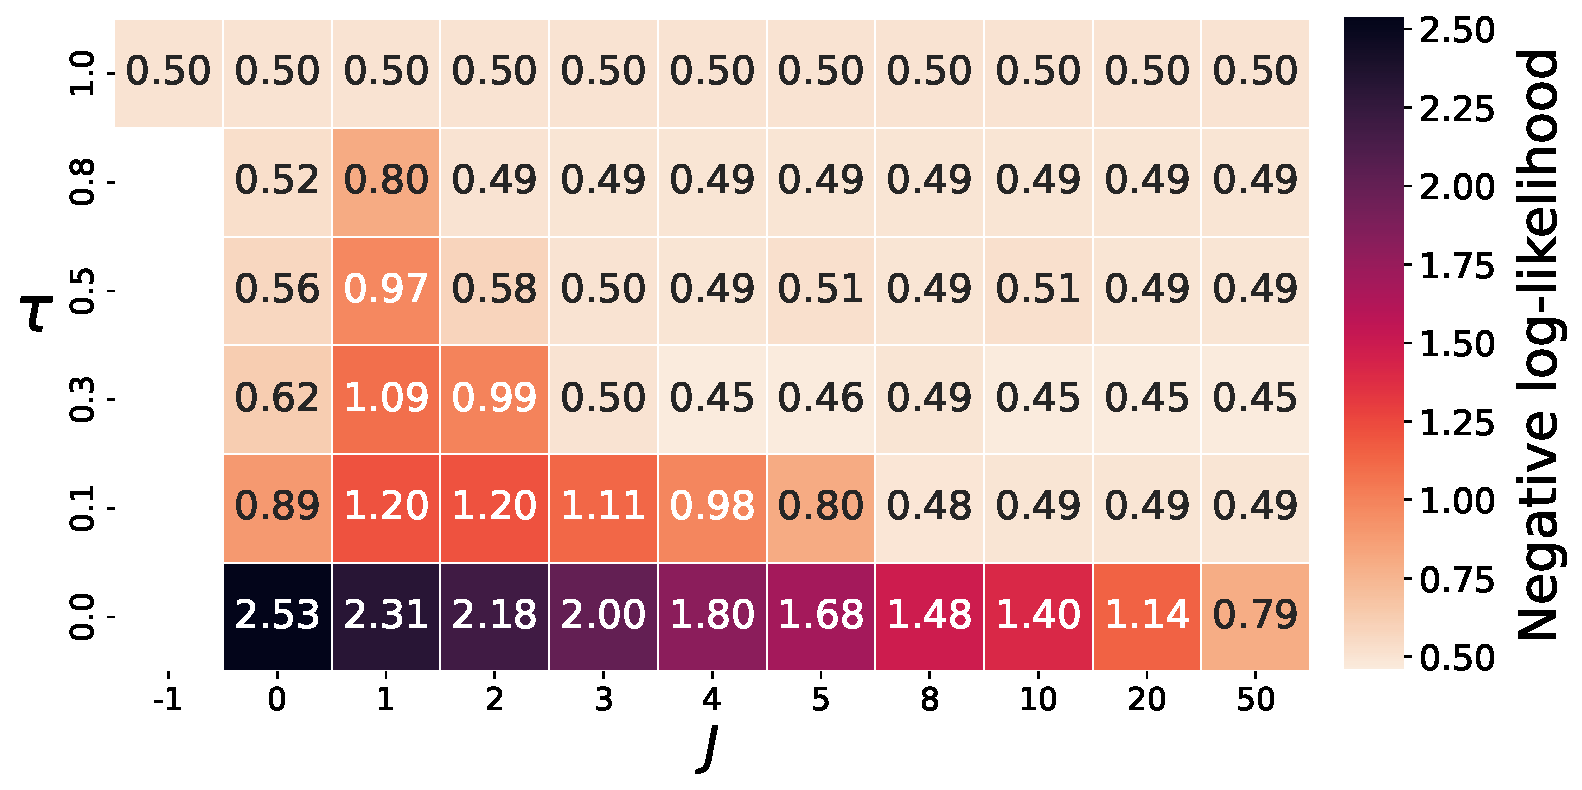
\includegraphics[width=0.7\textwidth]{images/rsgm/s2_heatmap.pdf}

	\caption{
		Ablation study on the denoising score matching (DSM) loss \(\ell_{t|0}\) when combining the heat kernel truncation and the Varadhan approximation: \(\nabla_{x_t} \log p_{t|0}(x_t|x_0) \approx \mathbbm{1}(t \le \tau) \exp^{-1}_{x_t}(x_0) + \mathbbm{1}(t > \tau) S_{J,t}(x_0,x_t)\).
	}
	\label{fig:s2_heatmap}
\end{figure}

\subsection{Torus}

\paragraph{Data}

The synthetic data trained on consists of a wrapped Gaussian distribution on \(T^n\) with uniformly chosen random mean and standard deviation of \(0.2\).
Such a distribution is defined by taking the density of a Normal distribution in the tangent space of the manifold at the mean and passing it through the exponential map at the mean.

\paragraph{Architecture}

To parametrize the vector field on \(\mathbb{T}^n\) we use a single filed per dimension pointing in a consistent direction around the i\(^{th}\) component in the product, with unit norm.

\paragraph{Models}

All models were trained with the same 3 layer, 512 units per layer MLP across different dimension sizes.

\paragraph{Optimization}

The models are optimized for 50\(k\) iterations.
The RSGM models are trained with both the implicit score-matching loss and the sliced score-matching loss.

\subsection{Special Orthogonal group}

Applications of orthogonal constraints span various fields, such as protein docking with ligands binding pose prediction \parencite{ganea2022independent}, robotics and Computer vision with rigid body transformation estimation \parencite{barfoot2011Pose,deepdirectstat2018}, and medical imaging for data alignment \parencite{hou2018Computinga}.

\paragraph{Data}
We consider the synthetic dataset consisting of samples in \(\mathrm{SO}_3(\R^d)\)\footnote{This manifold is \(3\)-dimensional.
} from the
mixture distribution with density
\(p(\mathrm{Q})=\frac{1}{K} \sum_{k=1}^K
	\mathrm{N}^W(\mathrm{Q}|\mathrm{Q}_k,\sigma_k^2)\) with \(K \in \N\),
where for any \(k \in \{1, \dots, K\}\), we have that
\(\mathrm{Q} = \mathrm{Q}_k\exp_{\m{I}}[\sigma_k \hat{z}]\) with
\(z \sim \mathrm{N}(0, \m{I}_{\R^3})\) satisfies
\(Q \sim \mathrm{N}^W(\mathrm{Q}_k, \sigma_k)\) and \((\cdot)^{\wedge} : \R^3 \rightarrow \mathfrak{so}(3)\).
For any \(k \in \{1, \dots, K\}\), we set \(\mathrm{Q}_k \sim \mu\) where \(\mu\) is the uniform distribution on \(\mathrm{SO}_3(\R)\) and \(\sigma_k^2 \sim \mathrm{IG}(\alpha=100, \beta=1)\), where \(\mathrm{IG}\) is the inverse Gaussian distribution.
We choose \(K=32\) mixture components.
We showcase a conditional sampling extension of our model---see \cref{sec:conditional_rsgm} for more details--- by targeting individual mixture components \(p(Q|k)\).
Our model is trained using the \(\ell_{t|0}\) (DSM) loss along with the Varadhan asymptotic approximation, see \eqref{eq:varadhan}.

\paragraph{Architecture}
To parametrize the vector field, we rely on the basis of the Lie group, \(\mathfrak{so}(n)= \cbrcolon{\mathrm{A} \in \mathrm{M}_d(\R)}{\mathrm{A}^\top = -\mathrm{A} }\) given by \(\mathrm{E}_{ij} = \mathrm{U}_{ij} - \mathrm{U}_{ji}\) for \(i, j \in \{1, \dots, d\}\) with \(i < j\) and \(\mathrm{U}_{ij} = (\delta_{ij}(k,\ell))_{1\leq k, \ell \leq d}\), which induces a basis on the tangent spaces \(\mathrm{T}_{\mathrm{Q}} \mathrm{SO}_d\) for any \(\mathrm{Q} \in \mathrm{SO}_d(\R)\) given by \(\{\mathrm{Q} \mathrm{E}_{ij}\}_{1 \leq i<j \leq d}\).
This is the divergence-free vector field approach described in \cref{sec:riem-score-appr}.

\paragraph{Models}
We compare our proposed approach against Moser flows~\parencite{rozen2021moser} and a wrapped-exponential baseline \parencite{falorsi2019reparameterizing} defined as the pushforward along the transformation \(\R^3 \xrightarrow[]{F^{-1}_\theta} \R^3 \xrightarrow[]{g} \R^3 \xrightarrow[]{\wedge} \mathfrak{so}(3) \xrightarrow[]{\exp} \mathrm{SO}_3(\R)\) with \(F^{-1}_\theta\) denoting the approximate time-reversed diffusion, \(g\) denoting the radial operator defined by \(g: \ x \mapsto 2\pi \tanh(\|x\|) x / \|x\|\), \((\cdot)^{\wedge} : \R^3 \rightarrow \mathfrak{so}(n)\) the isomorphism given by the basis on \(\mathfrak{so}(3)\) and \(\exp\) the matrix exponential.
The radial \(g\) operator's constant \(2\pi\) is chosen as the injectivity radius of the group so that the transformation \(\tanh \circ \wedge \circ \exp\) is injective (the set of elements with no preimage is then only the cut locus which is known to have measure zero).
Henceforth, this wrapped-exponential transformation cannot be bijective, it is either injective \emph{or} surjective depending on the choice of radius in the radial operator \(g\).

\paragraph{Optimization}
Models are trained for \(100k\) iterations.
The Riemannian SGM is trained with the Varhadan approximation of the denoising score-matching loss (DSM)~\cref{sec:riem-score-appr}, and the wrapped-exponential model relies on the exact DSM loss.
After a first hyperparameter exploration, a grid search is performed over \(\texttt{learning\_rate} \in [2e-5, 4e-5]\), for SGMs over \(\beta_f \in [0.5, 1, 2, 4, 6, 8, 10]\) and for Moser flows over \(K \in [1000, 10000]\) and \(\lambda_{\min} \in [1, 10, 100]\).
